% This template was originally by R. Jacob Vogelstein
% Updated on March 1, 2010 by Noah J. Cowan

\documentclass[12pt,oneside]{thesis}

\usepackage[superscript]{cite}
\usepackage{amsmath,amsfonts,amstext}
\usepackage{url}
\newcommand{\degree}{\ensuremath{^\circ}}
\usepackage{graphicx}
\usepackage{epstopdf}
\graphicspath{{./figs/}}
%\usepackage{fixltx2e}
\usepackage{array}
% wrapfig is fragile: use sparingly
\usepackage{wrapfig} 
%\usepackage{times}  % Use this for ugly fonts

\usepackage{upgreek}
\usepackage{textgreek}
\usepackage{hyperref}
\usepackage{setspace}

\usepackage{booktabs}
\usepackage{multirow}
\usepackage{longtable}
\usepackage[font=singlespacing, labelfont=bf]{caption}
%\usepackage{CV}

\usepackage{enumitem}
\newlist{inlinelist}{enumerate*}{1}
\setlist*[inlinelist,1]{%
  label=(\arabic*),
}

\usepackage{fancyhdr}    % Use nice looking headers along with the required footer page numbers   
%\usepackage[hypertex]{hyperref}

%Define the header/footer style
\pagestyle{fancy}
\fancyhf{}
\setlength{\headheight}{15pt}
\lhead{\leftmark}
\cfoot{\thepage}
\renewcommand{\headrulewidth}{0pt}
\fancypagestyle{plain}{% Redefine ``plain'' style for chapter boundaries
\fancyhf{} % clear all header and footer fields
\fancyfoot[C]{\thepage} % except the center
\renewcommand{\headrulewidth}{0pt}
\renewcommand{\footrulewidth}{0pt}}

\makeatletter
\let\@currsize\normalsize
\makeatother

\tolerance=10000

%\makeglossary % enable the glossary

% DAN ADDED
\usepackage{appendix}
\usepackage{pdfpages} 	
\usepackage{amssymb}


% See:
% http://tex.stackexchange.com/questions/11579/captions-for-figures-in-listoffigures
% http://tex.stackexchange.com/questions/82858/how-to-get-thumbnails-in-a-list-of-figures
\newlength{\lofthumbsize}
\setlength{\lofthumbsize}{8em}

\newif\iflofimage
\DeclareRobustCommand*{\lofimage}[2][]{%
\iflofimage
$\vspace*{-1.2\baselineskip}
  \hbox to .7\columnwidth{\hss\raisebox{1\baselineskip}{\includegraphics[{width=\lofthumbsize,keepaspectratio=true,#1}]{#2}}\hss}%
$%
\vspace*{0.2\baselineskip}
\newline
\fi
\ignorespaces
}

\begin{document}

\title{Interfacial Microrheology of Biological Films}
\author{Daniel B. Allan}
\degreemonth{December}
\degreeyear{2014} 
\dissertation
\doctorphilosophy
\copyrightnotice


% add your chapters, best way is to have separate TeX files for each chapter
%% FRONTMATTER
\begin{frontmatter}

% generate title
\maketitle

\begin{abstract}

Abstract goes here.

\vspace{1cm}

\noindent Primary Reader: Some Person\\
Secondary Reader: Someone Else

\end{abstract}

\begin{acknowledgment}

Thanks!

\end{acknowledgment}

% generate table of contents
\tableofcontents

% generate list of tables
\listoftables

% generate list of figures
\lofimagetrue
\twocolumn
\begingroup
\let\onecolumn\twocolumn
\listoffigures
\endgroup
\onecolumn
\lofimagefalse

\end{frontmatter}

% !TEX root = root.tex
\chapter{Introduction}
\chaptermark{Introduction}

\section{Overview and Significance}

It was the best of times, it was the worst of times.

\section{Background}

\subsection{Rheology}

\subsubsection{Fundamentals}

Hooke's Law describes a solid as an idealized spring. A small deformation requires an applied force. The larger the deformation, the larger the requisite force, but the force in no way depends on the \emph{rate} of the deformation: fast and slow cost the same. A viscous liquid, as described by Newton's laws, behaves in a complementary way: it resists a small strain with a force proportional to the rate of strain but independent of the magnitude of that strain.

Real materials deviate from these simple pictures in two ways. First, if the force or deformation is large, the relationship between the applied stress and the strain (or, for liquids, strain rate) becomes more complicated than simple proportionality; the response is nonlinear. Second, even if the forces and deformations are small, some materials respond with both solidlike and liquidlike characteristics. For example, when a true solid is subjected to a constant force, it deforms at first and holds that shape henceforth, but a solid with liquidlike characteristics might slowly continue to deform overtime, creeping under the sustained force. Likewise, a liquid with solidlike characteristics might flow under an applied force but recoil slightly when the force is removed. Materials like these are viscoelastic.\cite{Ferry1980}

The theory of linear viscoelastic materials begins with a constitutive relation---a rheological equation of state, relating stress $\sigma$ to strain $\gamma$. The equation states that changes in strain are linear. The shear modulus $G$ is a memory function representing the ratio of stress to strain through a given strain history.

\begin{equation}
  \label{eqn:linear-constituive}
  \sigma(t) = \int_{-\infty}^t G(t - t')\dot{\gamma}(t')\, dt'
\end{equation}

\noindent Let us apply this principle to a simple oscillatory experiment, where a material is periodically deformed with some amplitude $\gamma_0$ at some frequency $\omega$.

\begin{equation}
  \gamma(t) = \gamma_0 \sin \omega t
\end{equation}

\noindent Eq. (\ref{eqn:linear-constituive}) gives

\begin{equation}
  \begin{aligned}
    \sigma(t) &= \int_0^\infty G(t - t') \gamma_0\,\omega \cos(\omega t')\, dt'\\
    &= \gamma_0\,\omega \int_0^\infty G(\Delta t) \cos[\omega (t - \Delta t)]\, d\Delta t\\
    &= \gamma_0 \left(\left[\omega \int_0^\infty G(\Delta t) \sin \omega \Delta t\, d\Delta t \right] \sin \omega t + \left[\omega \int_0^\infty G(\Delta t) \cos \omega \Delta t\, d\Delta t \right] \cos \omega t \right)
  \end{aligned}
\end{equation}

Because the bracketed factors depend only on $\omega$, we can define new functions $G'(\omega)$ and $G''(\omega)$, giving

\begin{equation}
  \sigma(t) = \gamma_0\, (G'(\omega) \sin \omega t + G''(\omega) \cos \omega t).
\end{equation}

The storage modulus $G'(\omega)$ gives the solidlike response, in phase with the oscillatory strain $\gamma(t)$, and the loss modulus $G''(\omega)$ gives the liquidlike response, 90$^\circ$ out of phase. They comprise the real and imaginary parts of the complex shear modulus, $G^*(\omega) = G'(\omega) + iG''(\omega)$.

\subsubsection{Measurement Techniques}

There is a large family of well-established techniques for measuring a material's frequency-dependent shear modulus $G^*(\omega)$. The stress--strain relationship can be probed in either direction, by applying a certain stress and measuring the resultant shear or by measuring the stress necessary to enforce a certain shear. For example, a creep experiment measures the strain in response to a sudden stress, whereas a stress relaxation experiment measures the stress following a sudden strain. Both of these are transient experiments, observing the material's response as a function of time after a brief change. Oscillatory experiments provide complimentary information, applying a periodic stress or strain at some frequency $\omega$, qualitatively probing the same response as a transient experiment at time $t=1/\omega$. Oscillatory experiments are especially important for probing high frequencies.

Shear rheology measurements, whether transient or oscillatory, strain-controlled or stress-controller, can be performed in many different geometries. Important ones include simple shear flow (Couette flow) between sheared parallel plates or, much more commonly, between rotating coaxial cylinders; flow inside a rectangular slit; torsion between two parallel plates; and torsion between a cone and plate.

All of these are, of course, subject to limitations. In oscillatory experiments the inertia of the rotating tool can dominate the shear response of the sample at  high frequencies. And all experiments contend with the problem of slip, the possibility that the sample might slip along a bounding surface where its velocity was assumed to be zero.

\subsection{Interfacial Rheology}



%On the Superficial... http://archive.org/stream/scientificpapers03rayliala/scientificpapers03rayliala_djvu.txt

Bicone ref

ICR

Visit vendor website for list of other geometries

Bo heuristic and Bo reality
\subsubsection{Theory}
\subsubsection{Measurement Techniques}
\section{Microrheology}
\subsection{Fundamentals}

\begin{equation}
  m\dot{v}(t) = f_R(t) - \int_0^t\zeta(t-t')v(t')\,dt'
\end{equation}

\begin{equation}
  m\left[s\tilde{v}(s) - v(0)\right] = \tilde{f}_R(s) - \tilde{v}(s)\tilde{\zeta}(s)
\end{equation}
\begin{equation}
  \tilde{v}(s) = \frac{\tilde{f}_R(s) + mv(0)}{ms + \tilde{\zeta}(s)}
\end{equation}

\begin{equation}
  \langle v(0)\tilde{v}(s) \rangle = \frac{\langle v(0)\tilde{f_R}(s)\rangle + m \langle v^2(0)\rangle}{ms + \tilde{\zeta}(s)}
\end{equation}

$\frac{1}{2}m\langle v^2(0) = \frac{1}{2}k_B T$

\begin{equation}
  \langle v(0)\tilde{v}(s) \rangle = \frac{Nk_B T}{ms + \tilde{\zeta}(s)} = Nk_B T \tilde{\zeta}^{-1}(s) = Nk_B T \tilde{M}(s)
\end{equation}

\begin{equation}
\end{equation}

\begin{equation}
\end{equation}

\begin{equation}
\end{equation}

\begin{equation}
\end{equation}

\begin{equation}
\end{equation}

\begin{equation}
\end{equation}

FLUCTUATION-DISSIPATION -- classic and quantum

\subsection{Interfacial Microrheology}

\subsection{Passive Microrheology}
HISTORY: Tracking By Hand


\subsection{Active Nanowire Microrheology}

Ways to track wires

\section{Protein Layers}
\section{Bacterial Biofilms}
\section{Cystic Fibrosis}
% !TEX root = root.tex
\chapter{Experimental Methods}
\chaptermark{Methods}

\section{Particle Tracking Experimental Design}

Time-lapse videos of particles in a sample are the raw data in particle tracking experiments. Collecting videos with the highest possible quality---in short, well defined particles with high contrast against a uniform background---simplifies data analysis and enables reliable interpretation. Here we address three critical factors that influence video quality: the particles, the microscope, and the camera. Optical properties of the sample under investigation also strongly impact the quality of videos that can be acquired, but those factors are typically beyond a researcher's control.

A variety of particles and illumination schemes have been used for particle tracking, including micron-sized colloids imaged via brightfield illumination \cite{Crocker1996}, gold nanoparticles via darkfield microscopy \cite{Martin2002a}, and fluorescent particles via fluorescence microscopy\cite{Nance2012}.

Bright, photostable, internally-labeled fluorescent polystyrene nanospheres are commercially available. Particles can alternatively be externally labeled by chemically conjugating fluorescent dye to functional groups on the particle surface. Internal labeling is often preferable, as it is less likely to change the surface properties of the particle and alter the particle�s interaction with the samples of interest, compared to external labeling. Many fluorescent dyes, with various chemical reactivities, are commercially available, though photostable dyes with high quantum yield and extinction coefficient should be selected whenever possible [Murphy]. The color of the fluorophore is another critical consideration. Biological specimens often have high autofluorescence, especially at shorter excitation wavelengths, which can interfere with particle detection and tracking. Red or dark red fluorescent dyes may be advantageous [Rust 2011; Schuster 2014], if a light source and detection scheme optimized for such dyes are available. 

Although some research groups use microscopes specially designed and optimized for particle tracking [Braeckmans chapter], custom-built instrumentation usually is not required. In fact, particle tracking videos can be collected using hardware common in biomedical research labs and core facilities\cite{Crocker2007}. For tracking of fluorescent particles, a widefield microscope with epifluorescence illumination and appropriate fluorescence filter sets is typically used. Objectives with large numerical aperture are ideal for high resolution particle tracking, since they collect more light, and tracking precision is proportional to the square root of the number of photons emitted by a fluorescent particle\cite{Crocker2007}. A high-powered light source, such as a mercury or metal halide arc lamp, should be used at its highest intensity setting. Then, the exposure time of the camera should be adjusted so that the image is neither under- nor over-saturated\cite{Crocker2007}. This procedure will minimize particle tracking errors, as discussed in a later section. The microscope should be placed on a pneumatic vibration-isolation table to dampen any external vibrations, such as from footsteps and lab equipment. If the microscope stage is to be heated for the experiment, the temperature should be at equilibrium before collecting tracking videos, to prevent sample drift arising from expansion or contraction of microscope components.

In fluorescent particle-tracking experiments, a sensitive (high quantum efficiency), low-noise camera is essential for precise particle tracking. The best choice is an electron-multiplying charge coupled device (EMCCD) camera, though scientific complementary metal oxide semiconductor (sCMOS) cameras can be used as well [Small]. The required frame rate will depend on the particle dynamics and research question. Some have found 15 frames per second to be sufficiently fast for studying transport of particles with diameters on the order of 100 nm in biological fluids and tissues, including mucus [Lai, Suk, Schuster], vitreous\cite{Xu2013}, and brain tissue\cite{Nance2012}. Faster frame rates will be necessary for studying more rapid movement. If the exposure time can be set independently of the frame rate, the exposure should be no longer than necessary to achieve bright particle images. The rationale behind this guideline will be discussed in the section on errors in particle tracking. Although particle tracking videos are large files, it is important that the data be saved in a lossless file format that does not compress the file by discarding information\cite{Crocker2007}.

Two rules should be kept in mind when preparing samples for particle tracking experiments. First, when possible, the chamber containing the sample should be well sealed to minimize sample evaporation and convective flow during the experiment\cite{Savin2005}. Second, the particle concentration must be appropriate for visualizing and tracking individual particles. The average particle spacing must be larger than the average particle displacement from frame to frame, or else the paths of multiple particles will intermingle, making it difficult to accurately reconstruct individual trajectories\cite{Crocker1996}. If the particles are moving very rapidly, a faster frame rate can be used, but if that is not sufficient or feasible, a new specimen with lower particle concentration should be prepared.

\section{Wire Fabrication}

% !TEX root = root.tex
\chapter{\label{chap:trackpy}Software Development: A Modern Particle-Tracking Toolkit}
\chaptermark{Software}

A large portion of my thesis effort has been devoted to the development of particle tracking and data analysis software, used for my own soft matter research and the work of others in our group. It is also being adopted by other soft matter researchers at Harvard, Princeton, Oxford, U. Chicago, U. Penn, and more. Relying on the growing open-source scientific software community, I have leveraged free, widely-used code for core functionality. By contributing my own particle tracking and data analysis code back to the community, I have increased the impact of the work and encouraged others to share their own improvements to my code, from which all users benefit.

One fast-growing product of this community is the notebook, a standard, browser-based record of code with figures, explanatory text and equations, and links and references. As recently outlined in an article published in \emph{Nature}\cite{Shen2014}, notebooks are making data analysis easier to record, understand, and reproduce. Many authors are publishing notebooks alongside papers, providing the detail that is essential for others to reproduce the work in a reasonable time scale.

\section{Introduction}

Particle tracking is an extremely powerful technique used across many disciplines of science. It has been used to directly image atomic rearrangements in silica glass\cite{Huang2013a}; to image stress and strain in drying colloidal films\cite{Xu2013a}; to image pleats in crystals on curved surfaces\cite{Irvine2010}; to [add biophys. examples].

\section{Review of the Crocker--Grier Particle Tracking Algorithm}

The particle tracking algorithm implemented by Crocker and Grier is performed in two steps: locating the particles in each frame and identifying the particles through time, linking coordinates into trajectories.

Trackpy implements the tracking algorithm of Crocker and Grier\cite{Crocker1996}. Theirs and similar algorithms\cite{Ghosh1994} have been widely used in the fields of colloid science, microrheology, biophysics, and biometrical engineering. The Crocker and Grier algorithm was originally implemented in the IDL programming language, but it has since been translated into various other languages, including Python, MATLAB, and C++. (A list of these related projects is maintained in the Trackpy Documentation in Appendix A.) Numerous alternative algorithms have been developed for tracking particles, which we discuss later.

In the algorithm of Crocker and Grier, particle coordinates are identified in four steps: 1) preparing the image using common image-processing techniques; 2) finding local maxima of brightness that may correspond to particles; 3) honing in on each candidate particle�s exact center with subpixel precision; and 4) discerning which of the candidates are true particles based on their morphology and measured brightness.

The software first prepares the images by applying a spatial bandpass filter, which uses a Fourier transform of the image to suppress features with small-scale variation (e.g., camera noise) and large-scale variation (e.g., uneven lighting). This effectively erases any objects in the background that are much smaller or much larger than the size of the particles. Next, the software identifies all local maxima in the processed image. These do not necessarily correspond to the particles' centers, but they provide an initial estimate of where particles may be found. If two or more local maxima are separated by a distance smaller than the particle diameter, they are assumed to belong to the same particle, and the software only retains the brightest one. Then, the software finds the intensity-weighted centroid (``center of mass'') of each spot, which is refined through iterative steps, using the whole region of the particle to resolve its center to a precision much better than 1 pixel. Finally, the software characterizes the neighborhood surrounding each spot by its total brightness, size, and eccentricity (deviation from circular shape). Using these attributes, spots that correspond to actual particles can be distinguished -- and the rest discarded -- with minimal user input. For example, true particles tend to appear bright and circular.

At this point, the software has identified the locations of particles in each frame. Next, the locations must be linked together across frames into particle trajectories. The algorithm robustly handles the complications of real trajectories: Particles are allowed to leave the frame, new particles are allowed to enter, and particles can even be tracked if they temporarily vanish and reappear nearby within a user-specified number of frames. If particles are well separated and moving slowly relative to the frame rate, the task of linking them is simple and unambiguous. If there are many particles in the field of view and they are moving quickly, the Crocker and Grier linking algorithm assigns particles in a way that minimizes the total length of the links. This is grounded in the statistics of random walks; a Brownian particle is most likely to be found near where it was last seen. The linking algorithm is rigorously correct for non-interacting Brownian particles [Crocker and Grier], and it is employed effectively in a variety of tracking applications. (See Section 4.3.2 for a more on trajectory linking.)

As the number of particles in view grows, resolving ambiguous networks is difficult. To simplify the problem, the algorithm requires the user to specify the maximum displacement allowed from one frame to the next. A good choice can simply be obtained by watching the particles and guessing the upper range of their movement between frames. For Brownian motion, the Stokes-Einstein equation provides a guideline as well. After trajectory linking is complete, inspect a histogram of displacements at the shortest time scale. If the histogram decays to zero just before the maximum displacement, then the choice of maximum displacement was proper. However, if the histogram stops abruptly at the maximum displacement, then redo trajectory linking with a larger maximum displacement. If, on the other hand, few displacements are nearly as large as the specified maximum displacement, then it may be set lower for better performance and accuracy.

To process a set of videos with automated tracking, only a few minutes of user attention are required to input parameters and check that they are suitable. A standard computer will typically be able to process at least one video frame per second, though this depends on the number of particles (and therefore the number of calculations needed for a single frame) in the video, as well as the exact automated tracking algorithm and implementation used. Thus, the software can process a typical video of a few hundred frames in a few minutes. The code will output the trajectories in a text file, spreadsheet, or database. Subsequent data analysis will depend on the scientific question under investigation. We discuss data analysis strategies in Section 3.3. 


\section{Particle Tracking in Trackpy}

A more detailed walkthrough in included among the extensive documentation and examples in the Appendix A.

\section{Subpixel precision and accuracy}

Understanding the precision and accuracy of particle localization is critical for conducting reliable particle tracking experiments. In fact, failure to recognize and account for imprecision and inaccuracy in tracking data can lead to misinterpretation (Deschout 2014; Parthasarathy). Precision refers to uncertainty in location, and is defined as the standard deviation of the measured locations when a single stationary particle is imaged and localized multiple times. In contrast, accuracy describes whether the position estimates deviate from the true particle position with systematic bias (Cheezum; Deschout). 

Tracking resolution (i.e., localization precision) is different than microscope resolution. As classically defined, microscope resolution is the minimum distance between two distinguishable points. The resolution of a traditional light microscope is approximately 250 nm, half the wavelength of visible light (Thompson). However, this limit does not apply to locating the center of one isolated point. Using an appropriate algorithm, it is possible to localize the center of an isolated particle or point source to better than the diffraction-limited resolution (Bobroff; Deschout 2014). In fact, researchers can routinely track particles with a lateral spatial precision of tens of nanometers or less using a standard light microscope (Crocker and Hoffman).
How is it possible to locate a particle�s center to better than pixel resolution? If a particle is only visible as one bright pixel, then we can only say that the particle is located somewhere in that pixel. But if the particle�s image spans multiple pixels -- ideally, more than three pixels across -- we can find its position with subpixel accuracy by taking the average position of these pixels, weighted by brightness. Alternative methods for calculating particle position with subpixel resolution are discussed in Section X.

\subsection{Static Error}

Tracking precision is subject to both fundamental and experimental limitations. The fundamental limitation is photon noise: a particle emits photons stochastically, and consequently, there is statistical uncertainty in locating the particle from its image (Fig. 9 and Table 1) (Ober). The size of this uncertainty is inversely proportional to the square root of the number of detected photons (Ober; Crocker).
Experimental limitations related to detector and specimen properties can also degrade localization precision. Detector noise, including dark current (thermally-induced electrons in the detector) and readout noise (errors in reading the number of photoelectrons built up in a pixel), can interfere with particle localization (Thompson; Deschout). Detector noise is greatly reduced in high-performance, cooled, EMCCD cameras. Specimen autofluorescence and out-of-focus background fluorescence can also reduce localization precision and accuracy, which can be an issue when tracking particles in a thick biological specimen using standard epifluorescence illumination. Image processing can remove some, but not all, of this background (Deschout 2014). Finally, lateral localization precision of fluorescent particles is best for particles located in the focal plane -- where the particle image is smallest, brightest, and closest to a Gaussian curve in shape -- and decreases with increasing distance from the focal plane (Savin 2008; Deschout 2014).
This inability to exactly localize particles has been referred to as static error, localization error, or random error (Savin and Doyle; Martin; Crocker). Static error adds a constant offset to the MSD, as derived previously (Martin): $\langle \Delta r^2 \rangle + 2*\epsilon^2$, where $\epsilon$ is the localization uncertainty. A perfectly immobilized particle will have a true MSD = 0 for all lag times, but because of static error, the actual measured MSD will be a non-zero constant, $\langle \Delta r^2 \rangle = 2*\sigma^2$ (Martin; Crocker). However, in most particle tracking experiments, the true underlying MSD is not known a priori, so it may not be immediately evident which component of the measured MSD is �true" and which is artifact.
In addition to the random error associated with camera noise and pixelation, particle localization is subject to systematic errors, wherein particles can be �biased� toward certain locations, such pixel centers. Several experimental details in both hardware and software are implicated in these errors (Crocker and Hoffman again). Of course, if the particles typically step much more than a pixel between frames, optimizing subpixel resolution is less important. Readers with applications where particles frequently move in subpixel steps are encouraged to consult the referenced literature and consider these details with care.

\subsection{Dynamic Error}

Additional error is introduced by motion blur. When a particle moves substantially during the camera exposure time, a blurred spot is recorded, representing the time integral of the particle�s location (Fig. 10 and Table 1). Particle motion during the exposure time reduces the observed MSD at short times for randomly diffusing particles, since they tend to revisit previously explored regions (Crocker and Hoffman; Berg). This effect has been called dynamic error (Savin and Doyle). In addition, particle motion increases static error, because motion blur reduces localization precision by roughly two-fold under typical experimental conditions, as compared to stationary particles (Deschout 2012).
Like static error, dynamic error can alter the measured MSD, and can thus introduce inaccuracies when using the MSD to calculate diffusion coefficients and viscoelastic moduli. Static error alone adds a constant offset to the MSD, which flattens the MSD at short time scales on a log-log plot, and makes diffusive motion appear sub-diffusive (Martin). Dynamic error, by itself, decreases the MSD at short time scales, which makes diffusive motion appear like active transport. Static and dynamic error act in opposite directions, so depending on which type of error is larger, one effect may dominate, or occasionally, the two effects may largely cancel each other (Savin and Doyle). Both sources of error are more pronounced at short time scales, when the true MSD is smaller.

\subsection{Experimental Best Practices to Minimize Error}
Prior to collecting data, it is critical that researchers consider how to minimize static and dynamic error, as they are difficult if not impossible to completely correct after the experiment. To boost signal-to-noise ratio and reduce static error, researchers should choose bright particles, a microscope objective with large numerical aperture, and a sensitive camera with low noise. The only way to reduce dynamic error is to use an exposure time that is small compared to the frame interval (Savin and Doyle; Crocker and Hoffman). Unfortunately, shorter exposure time also increases static error. A compromise is to use the longest exposure time possible without introducing large dynamic error. As a point of reference, for Brownian motion, an exposure time no longer than one quarter the frame interval will cause dynamic error of <10\% at the shortest time scale, and smaller dynamic error at longer time scales (Crocker and Hoffman).
After conducting an experiment, dynamic error is especially difficult to correct, because it is time-dependent and also depends on the underlying type of motion, which is often unknown (Savin and Doyle). Static error is simpler to quantify and correct ex post facto, since static error adds a constant offset to MSD regardless of the nature of particle motion. Static error can be estimated by tracking particles fixed to a coverslip under signal-to-noise conditions similar to those of the experiment, and then subtracted from the ensemble MSD. However, this simple approach may not precisely mimic the background noise in the experiment, nor the effect that motion blur has on static error. An alternative method has recently been proposed for measuring localization precision of moving particles, though this technique requires a custom microscope configuration (Deschout 2012). Tracking particles in water or other fluids of known viscosity and comparing their MSD to theory may also help reveal types and magnitudes of error. 
How much do researchers conducting particle tracking experiments need to worry about static and dynamic error? The answer depends both on the system under investigation and on the desired analysis. If the research objective is to precisely quantify diffusion coefficients or viscoelastic moduli, or to fit the data to a model, it is critical to consider error to ensure proper analysis -- especially if the imaging conditions were not ideal. In particular, higher spatial and temporal resolution are needed to accurately study particle motion at short times scales, where the MSD is smaller and the errors proportionally larger. However, if the research objective is to qualitatively compare the transport of two types of nanoparticles with very different behavior, such as mobile and immobile, moderate tracking errors require less thorough examination and are unlikely to alter the final conclusion. 

\section{Prediction Framework}

The Crocker--Grier particle tracking algorithm, at its simplest level, takes each particle in
the previous frame and tries to find it in the current frame. This
requires knowing where to look for it. The algorithm was developed to track particles undergoing Brownian diffusion,
in which a particle's velocity is uncorrelated from one
frame to the next. Therefore, a particle is statistically most likely to be found at or near is last known location. The particle in the current frame closet to a particle in the previous frame is likely to be the same particle.

Let's formalize this guessing as \emph{prediction}. Consider a function

\begin{equation}
P(t_1, t_0, \vec x(t_0))
\end{equation}

\noindent that takes the particle at position $\vec x(t_0)$ and predicts its
future position $\vec x(t_1)$. The optimal predictor for Brownian motion
is

\begin{equation}
P(t_1, t_0, \vec x(t_0)) = \vec x(t_0)
\end{equation}

\noindent which, of course, is also the simplest to implement.

The better our prediction about where to look in the next frame, the
more likely we will find the one and only particle we seek.
In practice, the algorithm looks for the particle in a circular region of radius
\texttt{search\_range}, centered on $P(t_1, t_0, \vec x(t_0))$. So to
successfully track particle $i$ puts a limit on the error in our
prediction:

\begin{equation}
\label{eqn:brownian-predictor}
\|P(t_1, t_0, \vec x_i(t_0)) - \vec x_i(t_1)\| \le \tt{search\_range}
\end{equation}

This favors a generous \texttt{search\_range}. However, if
\texttt{search\_range} is too big, then for each particle in the
previous frame there will be many possible matches in the current frame,
and so matching one frame to the next requires the computer to evaluate
an overwhelming set of possibilities, seeking the one that minimizes the total displacements of all particles. Tracking may become extremely
slow, the problem effectively intractable.
So for the Brownian $P$ above, \texttt{search\_range} must be bigger
than the largest particle displacement between frames, but smaller than
the typical spacing between particles\cite{Crocker1996}. If such a value does not exist, the Crocker--Grier algorithm is not effective.

However, if particle motion is not strictly Brownian, its velocity
probably \emph{is} correlated in time. We may be able to improve $P$. This 
is the justification for trackpy's prediction feature.

\subsection{Prescribed predictors}\label{prescribed-predictors}

Consider a toy example: a regular array of particles,
translating with constant velocity $v$. Figure \ref{fig:prediction-const-features}
shows the particles' positions in two consecutive frames.

    \begin{figure}
    \centering
    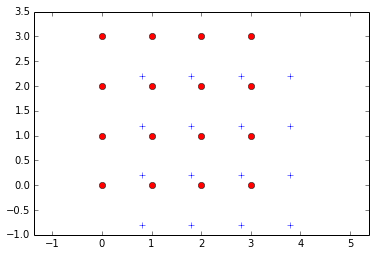
\includegraphics[width=\columnwidth]{prediction/prediction_4_1}
    \caption{\label{fig:prediction-const-features}An ensemble of particles moving under constant velocity. The red circles represent their positions at some time $t$, the blue crosses at some later time $t'$.}
    \end{figure}

\noindent Using the Brownian predictor, Eq. (\ref{eqn:brownian-predictor}), trackpy links the particles as shown in Figure \ref{fig:prediction-const-brownian-link}.

   \begin{figure}
    \centering
    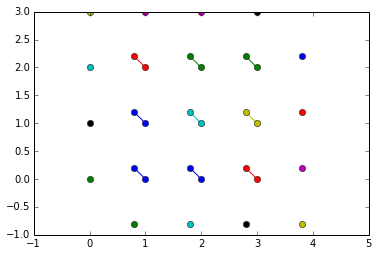
\includegraphics[width=\columnwidth]{prediction/prediction_7_0}
    \caption{\label{fig:prediction-const-brownian-link}An ensemble of particles moving under constant velocity are identified through time using a simple Brownian prediction, Eq. (\ref{eqn:brownian-predictor}). Features that have been identifies as belonging to the same trajectory are connected by a line. In this case, the identification is not correct.}
    \end{figure}
    
\noindent This is obviously not correct. Let us provide a $P$ which reflects this constant

\begin{equation}
\label{eqn:const-predictor}
P(t_1, t_0, \vec x_i(t_0)) = \vec x_i(t_0) + v(t_1 - t_0)
\end{equation}

\noindent The result is accurate (Figure \ref{fig:prediction-const-const-link}). To be clear, the predictor does not need to specify exactly where the
particle will be; it only must bias the search enough that the correct
identification will be made.

   \begin{figure}
    \centering
    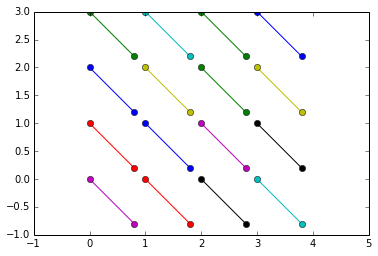
\includegraphics[width=\columnwidth]{prediction/prediction_9_1}
    \caption{\label{fig:prediction-const-const-link}An ensemble of particles moving under constant velocity are identified through time using a constant-velocity predictor, Eq. (\ref{eqn:const-predictor}). Features that have been identifies as belonging to the same trajectory are connected by a line.}
    \end{figure}

\subsection{Dynamic predictors}\label{dynamic-predictors}

In typical experimental conditions, the particles' velocities are not known ahead of time. It would be much better for the predictor to ``learn'' about
the velocities, and allow different particles to have different
velocities that can change over time. To accomplish this, $P$ will depend on more than $x_0$, $t_0$, and $t_1$; it will also depend on the particles' most recent velocities.

\begin{equation}
\label{eqn:adaptive-predictor}
P(t_1, t_0, \vec x_i(t_0)) = \vec x_i(t_0) + \frac{\vec x_i(t_0) - \vec x_i(t_{-1})}{t_0 - t_{-1}} (t_1 - t_0)
\end{equation}

There are a few caveats.
  If a new particle is in frame $t_i$ but wasn't in $t_{i-1}$, its velocity is unknown, but it is estimated using the velocity of the nearest existing particle. Of course, in the first frame, all
  velocities are unknown because
  there is no previous frame. Fortunately, even though particles may be in motion from the start, an initial guess
  of $v_0 = 0$ often gives acceptable results. In many cases, at
  least some of the particles are moving slowly enough that they can be
  tracked and their velocity can be obtained. Then, because particles with
  unknown velocity borrow the nearest known velocity, this may give the algorithm a foothold to track more particles
  in later frames. If that is not sufficient, a more accurate initial guess can be specified. This guess can be a constant velocity, a velocity profile, or N-dimensional velocity field.

As a demonstration, consider a three-frame sequence that starts
with small displacements and accelerates. With a simple Brownian predictor, tracking fails at the third frame (Figure \ref{fig:prediction-acceleration-brownian-link}). With the adaptive predictor, Eq. (\ref{eqn:adaptive-predictor}), tracking is accurate (Figure \ref{fig:prediction-acceleration-adaptive-link}).


   \begin{figure}
    \centering
    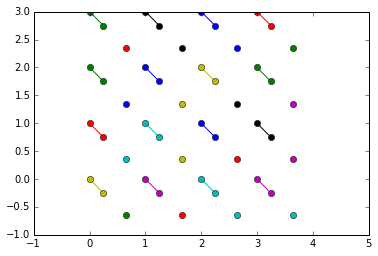
\includegraphics[width=\columnwidth]{prediction/prediction_14_1}
    \caption{\label{fig:prediction-acceleration-brownian-link}An ensemble of accelerating particles are identified through time using a simple Brownian prediction, Eq. (\ref{eqn:brownian-predictor}). The identification is incorrect.}
    \end{figure}
   

   \begin{figure}
    \centering
    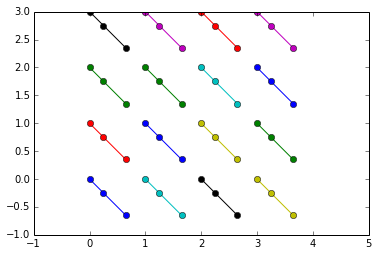
\includegraphics[width=\columnwidth]{prediction/prediction_16_1}
    \caption{\label{fig:prediction-acceleration-adaptive-link}An ensemble of accelerating particles are identified through time using a simple Brownian prediction, Eq. (\ref{eqn:adaptive-predictor}).}
    \end{figure}


    \subsubsection{Channel flow prediction}\label{channel-flow-prediction}

There are two special cases implemented by trackpy. The first is channel flow, in which velocities are relatively uniform in one
direction. For example, if the channel is in the $x$ (i.e. $\hat i$)
direction, particle velocities are very well approximated as

\begin{equation}
\vec v = \hat i v_x(y)
\end{equation}

\noindent where the velocity profile $v_x(y)$ is a smoothly-varying function
defined across the channel. The required inputs are the direction of flow and size of the bins used to
define the channel profile. The initial velocities can be specified or arrived at adaptively.

Figure \ref{fig:prediction-channel-brownian-link} shows an example. The simple Brownian prediction fails for the top row of particles at the edge of the channel. With a Channel Flow prediction, the tracking is accurate (Figure \ref{fig:prediction-channel-channel-link}).

   \begin{figure}
    \centering
    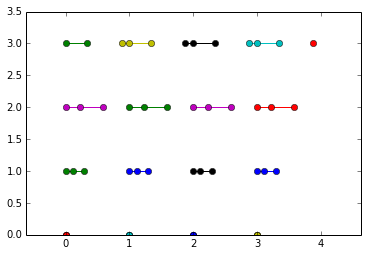
\includegraphics[width=\columnwidth]{prediction/prediction_20_1}
    \caption{\label{fig:prediction-channel-brownian-link}An ensemble of particle moving in simulated channel flow are identified through time using a simple Brownian prediction, Eq. (\ref{eqn:brownian-predictor}). The identification is incorrect.}
    \end{figure}

   \begin{figure}
    \centering
    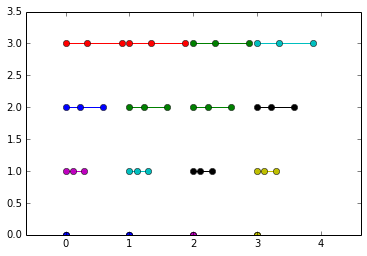
\includegraphics[width=\columnwidth]{prediction/prediction_22_1}
    \caption{\label{fig:prediction-channel-channel-link}An ensemble of particle moving in simulated channel flow are identified through time using a Channel Flow predictor.}
    \end{figure}
   

    \subsubsection{Drift prediction}\label{drift-prediction}
    
The second special case implemented by trackpy is drift prediction. At the interface, it is common to observed convective flows driven by air currents or heat from the illuminating lamp. In the final data analysis, this motion can often be subtracted away by adopting a reference frame set by the average velocity of the ensemble of particles. Likewise, tracking accuracy and performance is improved by forming a prediction based on the average velocity of the ensemble.

\section{Results}
\subsection{Accuracy vs. ``ground truth'' and vs. other approaches}
\subsection{Performance}
\section{Testing \& Reproducibility}

Trackpy is packaged with more than 150 automated tests: snippets of code that exercise a specific capability of trackpy by running toy examples and comparing the output to known correct results. For example, to test feature location, an automated test draws a simple image with several dots and checks that trackpy can locate the dots with a given precision.

Testing benefits a research code in more than one way. Most obviously, tests verify correctness and check special cases. Just as important, tests protect reproducibility. By codifying key results as tests, authors can be sure that these results cannot be broken inadvertently in the future. This empowers users who do not have familiarity with the whole codebase to make contributions and changes with confidence that they will not have unintended consequences. When revisions are submitted to trackpy, a web service automatically executes all the tests, and it alerts the user if any tests fail under the proposed change. Finally, the test suite complements the documentation. Technical users and potential contributors can browse it as a comprehensive demonstration of the ways in which the authors imagined the code would be used.

Trackpy has an unusual level of testing for a code from an academic lab. But the time invested has been worthwhile: it ensures that any research that depends on the code is grounded in a rigorous, scientific approach to software development. This guarantee earns the confidence of other researchers who decide to use, cite, or contribute to the codebase. It thereby increases the code's longevity and the impact of the development effort.

As trackpy is improved and changed, old research code may cease to reproduce exactly the same results. Testing help ensure that any such "breaking changes" are made deliberately and can be documented. To avoid breaking old code altogether, researchers can make note of which specific version of trackpy was used for a given project and roll back to that version when revisiting the research. Several new projects such as Docker, Dexy, and hashdist [any academic citations for these?] address this need: they recreate complete computing environments, making it possible reproduce research using the specific original versions of all the relevant software. These tools are especially powerful in simulation research, where the entire research project can reproduced on a computer. But they are also useful in experimental science, covering every step after data collection up to the production of the published figure.

\section{Conclusion}
\subsection{``A Modern Approach''}
Trackpy is distinguished among niche academic codes by its careful adherence to the best practices of the open source software community. The most important are code review and open discussion before each revision, automated testing, complete API documentation. Also, code comprehensibility and modularity are key design considerations. Code that merely works is not necessarily easy to test, maintain, extend, or reuse.

Code for academic use is typically developed for a single research project, often by a single researcher, at least at first. Trackpy has benefitted from its co-development by three different researchers working in separate groups at separate institutions on projects with vastly different priorities. The core functionality of trackpy was useful to all, and the healthy tension in the project drove the development of extensible, reusable code. In addition to the core developers, collaborators and other researchers used trackpy actively during its development. Their use of the cutting-edge code demanded stability and thorough documentation. As the project matured, a wider community of users discovered it and found it useful.

\subsection{Measuring Success}
The scientific software community has not settled on a single metric for the success of academic software. In the three years since the first lines of code were written, trackpy has supported published research from several academic research groups; trackpy has been downloaded thousands of times through the Python Package Index, though it is impossible to know if the recipients were genuine users; trackpy has been adopted by users from about ten top academic research institutions known to the authors. Most importantly, trackpy has benefitted from code contributions offered by those users, comprising both software experts and relative novices.

Particle tracking is a general problem in a number of fields, and thanks to the pioneering efforts of John Crocker, David Grier, and Eric Weeks, it has a strong tradition of open source code supporting first-rate research.

\subsection{Future Directions}

Trackpy can increase its impact and extend its applicability by incorporating algorithms and strategies from outside the colloids literature and the software lineage of Crocker and Grier. Researchers in the biological and biophysics communities also use these tools, but they have developed additional methods to solve more complicated image analysis problems. For example, in biological contexts, features must be located amidst a complex, busy environment where they are more difficult to distinguish and the methods discussed above can be insufficient to extract them. Tracking and the notion of a trajectory can be subtler, as features might split or merge with each other.

Separately, the scientific Python community continues to grow and develop ever more powerful tools for exploring, processing, and presenting data. Trackpy will build on this ongoing progress, providing tools specific to the needs of particle tracking.

% !TEX root = root.tex
\chapter{\label{chap:lysozyme}Linear and Nonlinear Microrheology of Lysozyme Layers Forming at the Air--Water Interface}
\chaptermark{Lysozyme Layers}

\section{\label{sec:introduction}Introduction}

When an aqueous protein solution forms an interface with air or an oil, the protein molecules can discover the interface through diffusion and adsorb.~\cite{Walder2011}  The adsorption process is commonly believed to include conformational changes to the protein that lift hydrophobic substructures out of the aqueous surroundings. As the interface ages, it becomes increasingly crowded with adsorbed protein, and its rheology changes dramatically.~\cite{Murray2011a}
The mechanical properties of interfacial protein layers are an important aspect of their biological function, as in films that form on lachrymal secretions~\cite{Rosenfeld2013} and saliva~\cite{Proctor2005}, and in their role in biomedical and food processing technologies.~\cite{Murray2002}  In particular, the mechanical behavior of interfacial protein layers can enhance the stability of droplets and bubbles in emulsions and foams.~\cite{SaintJalmes2005,McClements2004}
Protein layers are fragile, molecularly thin, and spatially heterogeneous films whose properties evolve with time. These features complicate traditional interfacial rheometry measurements and often make results difficult to interpret.  Recently, microrheology techniques have shown promise as an alternative method to characterize the evolving mechanical behavior of protein layers.  

As discussed in Chapter \ref{chap:methods}, the basic approach of microrheology, which is most often employed to study bulk materials, involves tracking the motion of colloids embedded in the material to probe its mechanical properties.  Passive microrheology connects Brownian fluctuations of colloids to a material's linear shear response. Active microrheology infers the drag on colloids driven by an external forcing and relates that drag to mechanical response through a linear or nonlinear model relating stress and strain.
Applying microrheology to an interfacial system like a protein layer presents particular challenges. The theory supporting microrheology assumes Stokes drag, which is subtle in two dimensions.~\cite{Saffman1975} Moreover, colloidal probes at an interface experience drag forces from both the interfacial layer and from the underlying subphase. Since no exact closed-form solution for the drag on a membrane-bound object exists, one must rely on the analytical and numerical approximations described in Section \ref{sec:interfacial-microrheology}.

Nevertheless, despite these challenges, microrheology has found increasing application in the study of films at fluid-fluid interfaces including not only protein layers~\cite{Lee2009, Lee2010, Lee2011, Dhar2010, Prasad2006} but also polymer layers,~\cite{Helfer2001, Kandar2010, Maestro2011} lipid monolayers,~\cite{Sickert2007, Choi2011, Kim2011, Park2011, Murakami2010} and particle-laden interfaces.~\cite{Wu2009a, Langer2012}  This work has included studies of both the linear shear rheology and nonlinear mechanical response of interfacial films.  Recently, the interfacial microrheology of layers of the protein $\beta$-lactoglobulin  at air-water and oil-water interfaces was investigated in a study that illustrated the promise of the technique.~\cite{Lee2010, Lee2011}  These experiments included both active and passive microrheology measurements that tracked the transition from viscous to elastic mechanical behavior as the layers form.  In both $\beta$-lactoglobulin adsorbing to the air-water and to an oil-water interface, the microrheology revealed a viscoelastic transition consistent with gel formation.  However, features of the transition, such as the rate of layer formation and degree of spatial heterogeneity, varied strongly between the two cases.~\cite{Lee2010, Lee2011} 

Although the viscoelastic transition in protein layers is often ascribed to network formation through intermolecular association,~\cite{Bos2001, Murray2002, Martin2002, Bantchev2003, Roberts2005, Murray2011a} and indeed the evidence from microrheology for gelation in $\beta$-lactoglobulin layers supports this scenario, other mechanisms for the onset of elasticity in  protein layers, particularly involving glass transitions, have been proposed.~\cite{Wierenga2006, Cicuta2005, Cicuta2003, Cicuta2007}  Therefore, in an effort to understand better those aspects of the viscoelastic transition in protein layers that are universal and those that are system specific, we have conducted a microrheology study of layer formation at the air interface of lysozyme solutions. As described in Section \ref{sec:background} below, layers formed by lysozyme at the air-water interface are good candidates for microrheology investigations.  Our study included passive measurements, which tracked the Brownian motion of spherical colloids at the interface, and active measurements in which the rotational motion of magnetic nanowires at the interface was employed to infer layer rheology.  The experimental methods are described in Section \ref{sec:procedures}.  As described in Section \ref{sec:results}, the passive measurements provide information about the linear frequency-dependent shear modulus of the layers, while the active measurements probe properties of the layer's nonlinear stress response.  Together the measurements track the interfacial rheology as it evolves through a viscoelastic transition with increasing layer age.  We discuss in Section \ref{sec:discussion} two possible frameworks for understanding this mechanical evolution:  gelation and the formation of a soft glass phase.  Finally, Section \ref{sec:conclusion} offers some conclusions from the study.



\section{\label{sec:background}Background}

Lysozyme is a single-chain globular protein comprised of 129 amino acids with molecular dimensions 3.0 $\times$ 3.0 $\times$ 4.5 nm$^3$ and molecular weight 14,300 g/mol.  The molecule is considered a ``hard'' protein that is rigid against conformational fluctuations, due in part to the presence of four internal disulphide bridges.  Correspondingly, lysozyme is stable against denaturation over an unusually large range of bulk solution conditions.  However, it readily adsorbs at the air-water interface, and interfacial rheometry measurements on mature interfacial layers reveal that they can acquire pronounced elasticity.\cite{Roberts2005,Malcolm2006}   The structural properties of adsorbed lysozyme layers have been studied in detail by neutron and x-ray reflectivity.\cite{Lu1998,Lu1999,Yano2009}   In addition, surface-sensitive spectroscopies have interrogated the conformational state of the absorbed molecules.\cite{Postel2003a,Lad2006a}  Interpretation of the reflectivity measurements has led to debate about the structure of adsorbed lysozyme.  While neutron reflectivity results indicate that the lysozyme retains its globular structure with no significant denaturation, time-resolved x-ray reflectivity results indicate that the molecules initially adsorb in a flat, unfolded structure.  Evidence for conformational changes is further provided by Fourier transform infrared spectroscopy, which indicates adsorbed lysozyme contains antiparallel $\beta$-sheets that are absent in the native structure.\cite{Lad2006a}   However, no direct evidence exists for the breaking of the internal disulphide bridges upon adsorption.  In absorbed layers of other protein species, such as  $\beta$-lactoglobulin, the formation of intermolecular disulphide bridges is seen as an important feature of layer formation.  By characterizing the viscoelastic transition in interfacial lysozyme layers, we seek to correlate properties of the viscoelastic behavior with possible structural models to provide further insight into the layer formation.

As described in the next section, we focus our study on lysozyme solutions with a fixed bulk concentration of 0.05 mg/ml, for which the reflectivity indicates dense monolayers form at the interface.\cite{Lu1998,Lu1999}  Specifically, this concentration is near the upper limit at which the thickness of mature layers, approximately 3.0 nm, is the same as more dilute layers.  At somewhat higher concentrations, the layer thickness increases, indicating a reorientation of the molecules at the interface, presumably due to crowding.  At far higher concentrations, lysozyme can form multi-layers at the air-water interface.  However, those concentrations are two orders of magnitude greater than in the present study.\cite{Lu1998}  Hence, in this study we consider monolayers of protein.


\section{\label{sec:procedures}Experimental Methods}

\subsection{\label{sec:sample_prep}Sample Preparation}

Lyophilized powder of chicken-egg lysozyme (Sigma Aldrich, purity of 98\%) was mixed gently \cite{Stathopulos2004} into 10 mM sodium phosphate buffer, pH 7.4, at room temperature to obtain solutions with 0.05 mg/ml protein. The solutions were employed within minutes of preparation.
For the measurements, samples were contained in a 1-cm inner-diameter cylinder with an inner surface whose bottom half was aluminum and top half was Teflon, so that when solution filled the cell to the appropriate level, the aluminum--Teflon seam pinned the air--water interface, creating a flat surface with no meniscus.
To begin, we filled the cylinder nearly to the seam with 0.5 ml of the protein solution. The age of the sample $t_a$ was measured from the moment the cell was filled with solution, creating a fresh interface with the air.
A spreading solution containing either spherical or nanowire colloids (discussed below) was prepared in advance and sonicated to disperse any colloidal aggregates. In addition to the colloids, the spreading solution contained equal parts buffer solution and isopropanol (IPA).~~To introduce the colloids to the interface, we touched a 10-$\mu$L droplet of the spreading solution to the surface. The solution wet the interface, depositing colloids uniformly over the surface.   Evaporation of the IPA typically caused convective flows at the interface that persisted for about one minute.  All measurements were performed only after these flows ceased.  After each experiment, the sample cell was cleaned thoroughly by scrubbing and sonicating in Alconox soap solution, acetone, and IPA, and then rinsed repeatedly in deionized water.

We note the presence of the IPA in the spreading solution could potentially influence layer formation at the interface.  Measurements of the sample mass over time indicated that some of the IPA evaporated within seconds while the rest mixed into the bulk, where if uniformly distributed it constituted at most 1\% of the solution.  While lysozyme is stable in such dilute IPA solutions at room temperature, the near-surface IPA concentration was likely larger at times shortly after application of the spreading solution, and the protein can denature at IPA concentrations above 20\%.~\cite{Velicelebi1979}  Further, even at concentrations below which the alcohol does not denature the lysozyme, its interactions with the protein could affect the protein's hydrophilicity, which would impact its adsorption properties.  To understand the possible effects of the IPA, we performed additional experiments using pure buffer as the spreading solution and found that the IPA did not significantly affect the interface's subsequent rheological properties.  Because we achieved better surface coverage of colloids by including IPA in the spreading solution, all results discussed here were obtained with this sample preparation. 

\subsection{Passive (Brownian) Microrheology}

For the passive microrheology measurements, we employed charge-stabilized polystyrene spheres (Interfacial Dynamics Corp.)~with radius 0.5~$\mu \text{m}$. We observed the colloids at the interface using an inverted bright-field microscope with a 40X objective (WD 2.7-3.7 mm, NA 0.6). A video camera (Nikon D3100) recorded a 300$\times$170-$\mu$m field of view at a rate of 30 frames per second, which set the shortest time over which probe motion could be characterized. (The exposure time was approximately 0.033 s, the inverse of the frame rate.)  Video was captured continuously, so that, in principle, probe trajectories could be followed for arbitrarily long durations. However, for analysis, the videos were divided into segments whose duration was restricted by the evolving dynamics at the interface during layer formation.

We extracted probe trajectories from the video using a custom Python implementation~\cite{trackpy} of the widely-used Crocker--Grier multiple-particle-tracking algorithm.~\cite{Crocker1996} 
We accounted for static and dynamic errors in the particle tracking, which can qualitatively distort microrheology measurements if left uncorrected.\cite{Savin2005}
Typically between 30 and 200 probes were in view at any time, constituting up to 0.3\% surface coverage. As the experiment proceeded, some probes encountered each other and aggregated, reducing the population of usable probes.  Also, we corrected for drift of the probes at the interface, which was more severe than in a typical bulk microrheology measurement, by subtracting the average velocity of the ensemble from that of each particle.

In general, particle mobility in an interfacial film is affected by drag from both the film and from the adjacent bulk fluid phases.  The bulk contribution is most important when the interfacial viscosity is small, and theories have been developed to separate the contributions.~\cite{Sickert2007, Levine2004, Dhar2006, Fischer2004a, Fischer2006, Levine2004a}  When the interfacial viscosity is large or the layer is viscoelastic, the subphase contribution is less important, and, as described below, the measurements on lysozyme layers were in this regime.  In this case, under appropriate conditions, one can obtain the frequency-dependent interfacial shear modulus $G^*(\omega)$ from the Brownian motion of the probes through a two-dimensional version of a generalized Stokes-Einstein relation,  \cite{Helfer2001, Maestro2011}
\begin{equation}
 G^*(\omega)=\frac{k_B T}{\pi i\omega \mathcal{F}_u \{\langle \Delta r^2 (t) \rangle \} }  \label{eq:StokesEinstein}
\end{equation}
where $\langle \Delta r^2 (t) \rangle$ is the particles' ensemble-average mean-squared displacement and $\mathcal{F}_u \{\langle \Delta r^2 (t) \rangle \}$ is its unilateral Fourier transform.  


\subsection{Active Microrheology}

\subsubsection{Magnetic Nanowire Probes.}~For the active microrheology measurements, we employed ferromagnetic nickel wires, whose fabrication has been described elsewhere.~\cite{Tanase2001} The wires, which had radius $R_w=0.175\ \mu$m and lengths $L$ from 5 to 30 $\mu$m, possessed a large magnetic moment ($\mu/\text{L} = 3\times10^{-14}\text{A}\cdot\text{m}^2/\mu\text{m}$) parallel to their axis. 
The wires were hydrophobically functionalized with n-octadecyltrimethoxysilane (OTMS) and spread onto the interface as described above. The functionalized wires make a contact angle at the air--protein solution interface of $\theta_c = 79\degree \pm 1\degree$, as determined previously,~\cite{Lee2010} implying the wires were approximately half-submerged.

\subsubsection{Microscopy with \textit{in situ} Magnetic Fields.}~Custom-built ``magnetic tweezers'' mounted on an inverted microscope (Nikon TE2000), were employed to apply time-dependent magnetic torques to an isolated wire at the interface.~\cite{Lee2009} The tweezers, consisting of two sets of four solenoids with ferromagnetic cores positioned symmetrically above and below the microscope focal plane, could produce fields in any direction within the focal plane.  A feedback mechanism in the electronics controlling the tweezers created rise times below 2 ms for a step change in the field.  A high-speed camera (Photron Fastcam), recording a 70 $\mu$m $\times$ 70 $\mu$m view at frame rates up to 1000 fps, captured the wire's motion.  The wire's orientation in each video frame was determined by analyzing the gray-scale image and treating the brightness of each pixel as an effective mass to calculate the principal ``inertial axis''.  With this procedure, we could resolve the orientation with an estimated precision of $\pm 0.1\degree$, a tenfold improvement over our previous method.~\cite{Lee2010} 
%With the wires pinned at the interface of the sample, we applied a magnetic torque $\Gamma_\text{mag.} = \vec{\mu} \times \vec{B}$ to rotate the wires in the plane of the interface.
%
%For a viscous interface, the relative contributions from interface and bulk are parameterized by $l_0=\eta_s/\eta$, the ratio of the surface viscosity $\eta_s$ to the bulk viscosity $\eta$. When the wire's length $L \lesssim l_0/10$, the rotational viscous drag $\zeta \approx 1.48L^2\eta_s$ \cite{Levine2004, Levine2004a}.

\subsubsection{Measurement Procedures and Analysis.}~Measurements of layer response to applied magnetic torques on wires were performed in the time domain using step changes in magnetic-field direction of 90\degree.~~Prior to the change in field direction, the field was oriented parallel to the wire, and hence to the wire's magnetic moment. Following the change in field direction, the wires experienced a magnetic torque, 
\begin{equation}
\Gamma_\text{mag} = \mu B \sin{\theta}
\end{equation}
where $\theta$ is the angle between the wire axis and the field, causing the wires to rotate in the plane of the interface.  Each measurement was repeated at several field values to test for linearity.  In most cases, fields between 30 and 50 Gauss were selected since they caused the wires to rotate with angular velocities that were well matched to the video frame rate.  At some later ages, when the layer imposed larger resistance to the wire rotation, field values up to 100 Gauss were employed.   In the low-Reynolds-number conditions of the measurement, the magnetic torque was balanced by the hydrodynamic drag and/or any elastic stresses from the interfacial layer and subphase.  In the case of a simple viscous drag, 
\begin{equation}
  \mu B \sin\theta = \zeta_r \dot{\theta}
  \label{eq:wire_eq_motion}
\end{equation}
\noindent where $\zeta_r$ is the drag coefficient.  The solution to Eq.~(\ref{eq:wire_eq_motion}) gives the resulting time dependence between the field and wire axis,\cite{Anguelouch2006b} 
\begin{equation}
  \theta(t) = 2 \tan^{-1} \left[ \exp \left( -\frac{\mu B}{\zeta_r} (t-t_0) \right) \right]
  \label{eq:sasha}
\end{equation}
where $t_0$ is an experimental parameter that accounts for uncertainty in the time that the wire begins rotating in response to the field change and can differ from zero by an amount up to the time between video frames.  For such a viscous interface, the relative contributions to the rotational drag from the interface and subphase are parameterized by the Saffman length, $l_0=\eta_s/\eta$, the ratio of the interfacial viscosity $\eta_s$ to the subphase viscosity $\eta$. When the wire's length $L < l_0/10$, the interface dominates the drag, and one finds \cite{Levine2004}

\begin{equation}
  \zeta_r = 1.48 L^2\eta_s
  \label{eq:wire_zeta}
\end{equation}
 
 As described below, in the active microrheology measurements on lysozyme layers, we observed that in some cases the rotational motion of the wires was consistent with simple viscous drag, Eq.~(\ref{eq:sasha}). However, in other cases, particularly at large layer age, we observed deviations from Eq.~(\ref{eq:sasha}) that we identify as a consequence of a nonlinear response by the layer to the stress imposed by the rotating wire.  Specifically, we find in these cases that the layer's response is well described as that of a non-Newtonian, power-law fluid. A power-law fluid is characterized by the stress-strain relation
\begin{equation}
\sigma = K\dot{\gamma}^{n}
\label{eq:pf}
\end{equation}
\noindent where $\sigma$ is the stress, $\dot{\gamma}$ is the strain rate, $K$ is known as the consistency, and the exponent $n$ is known as the flow index.  When $n=1$, Eq.~(\ref{eq:pf}) reverts to the stress-strain relation of a viscous liquid, while $n < 1$ and $n > 1$ correspond to shear-thinning and shear-thickening behavior, respectively. More generally, power-law fluids are a special case of Herschel-Bulkley fluids, which are characterized by a power-law stress-strain relationship above a yield stress, $\sigma_0$,
\begin{equation}
\sigma = \sigma_0 + K\dot{\gamma}^n
\label{eq:HB}
\end{equation}
\noindent Such non-Newtonian response is observed in a wide range of soft disordered materials including paints, plastics, polymeric solutions, and food products.~\cite{Alexandrou2001a}

Adopting a power-law fluid response like Eq.~(\ref{eq:pf}) to describe the wire motion under the influence of a magnetic torque leads to
\begin{equation}
  \mu B \sin\theta = (\zeta_{\text{pl}} \dot{\theta})^n.
  \label{eq:pf_wire}
\end{equation}
\noindent where the nonlinear drag coefficient $\zeta_{\text{pl}}$ has dimensions $(\text{N}\cdot\text{m})^{1/n}\cdot\text{s}$. An analytical solution to Eq.~(\ref{eq:pf_wire}) for $\theta(t)$ is not available; however, the inverse function $t(\theta)$ is:
\begin{align}
\label{eq:pf-solution}
  t(\theta) =&\left[\frac{\zeta_{\text{pl}}}{(\mu B)^{1/n}}\frac{n}{1-n}\right]\times\\ \notag
      &\sin^{1 - 1/n}\theta\ _2\text{F}_1\left(\frac{1}{2}, \frac{n-1}{2n}, \frac{3n-1}{2n}; \sin^2 \theta\right)\bigg\vert^{\theta}_{\pi/2} - t_0
\end{align}
\noindent where $_2\text{F}_1$ is the ordinary hypergeometric function and $t_0$ is the same small experimental parameter introduced in Eq.~(\ref{eq:sasha}).  As described below, we employ this form with $n < 1$ to analyze the wire rotation in the lysozyme layers.  However, we emphasize that Eq.~(\ref{eq:pf_wire}) should only approximate the torque relation in a power-law fluid.  A more precise relation would need to account fully for the flow generated in the layer around the wire, and specifically for its spatially varying shear gradients, and would not lend itself to straightforward comparison with experimental results.  Nevertheless, as shown below, Eqs.~(\ref{eq:pf_wire}) and (\ref{eq:pf-solution}) accurately capture the rotational motion of wires in lysozyme layers, indicating a nonlinear response characteristic of a power-law fluid.  


\section{\label{sec:results}Results}

\subsection{\label{sec:linear}Linear Rheology}

The rheology at an air interface with the lysozyme solutions evolves quickly following the formation of the interface, with viscoelastic behavior emerging within minutes in the passive measurements, consistent with reflectivity studies that indicate lysozyme adsorbs rapidly at the air-water interface.\cite{Yano2009}  Figure~\ref{fig:emsds} shows examples of the ensemble-averaged mean-squared displacement $\langle \Delta r^2(t) \rangle$ of the colloidal probes at several ages $t_a$ since creation of the interface.  For reference,  the mean-squared displacement of colloids at the air interface of pure buffer containing no protein is also shown.  In the absence of adsorbing protein, $\langle \Delta r^2(t) \rangle$ varies linearly with lag time indicating simple viscous drag with a viscosity consistent with water.  At the interface of the protein solution, the mobility of the probes evolves rapidly at early layer ages; therefore, $\langle \Delta r^2(t) \rangle$ at each age is determined based on video segments of limited duration (less than one minute).  For this reason, the maximum lag time $t$ is restricted to $ t \leq 1$ s to assure adequate statistics.  Within the resulting limited dynamic range, $\langle \Delta r^2(t) \rangle$ is well described as a power law, $\langle \Delta r^2(t) \rangle \sim t^{\alpha}$. As shown in Fig.~\ref{fig:power-law_expon}, the power-law exponent $\alpha$ steadily decreases with increasing age, signifying increasingly subdiffusive particle motion. Following analysis based on the generalized Stokes-Einstein relation, Eq.~(\ref{eq:StokesEinstein}), power-law behavior in the mean-squared displacements of the colloidal probes, $\langle \Delta r^2(t) \rangle \sim t^{\alpha}$ with $\alpha < 1$, implies the lysozyme layer's linear shear modulus, $G^*(\omega) = G'(\omega) + iG''(\omega)$, has power-law frequency dependence, $G'(\omega) \sim G''(\omega) \sim \omega^{\alpha}$.~\cite{Mason2000}  The significance of this power-law frequency dependence and its evolution with layer age is discussed in Section \ref{sec:discussion} below.


\begin{figure}
 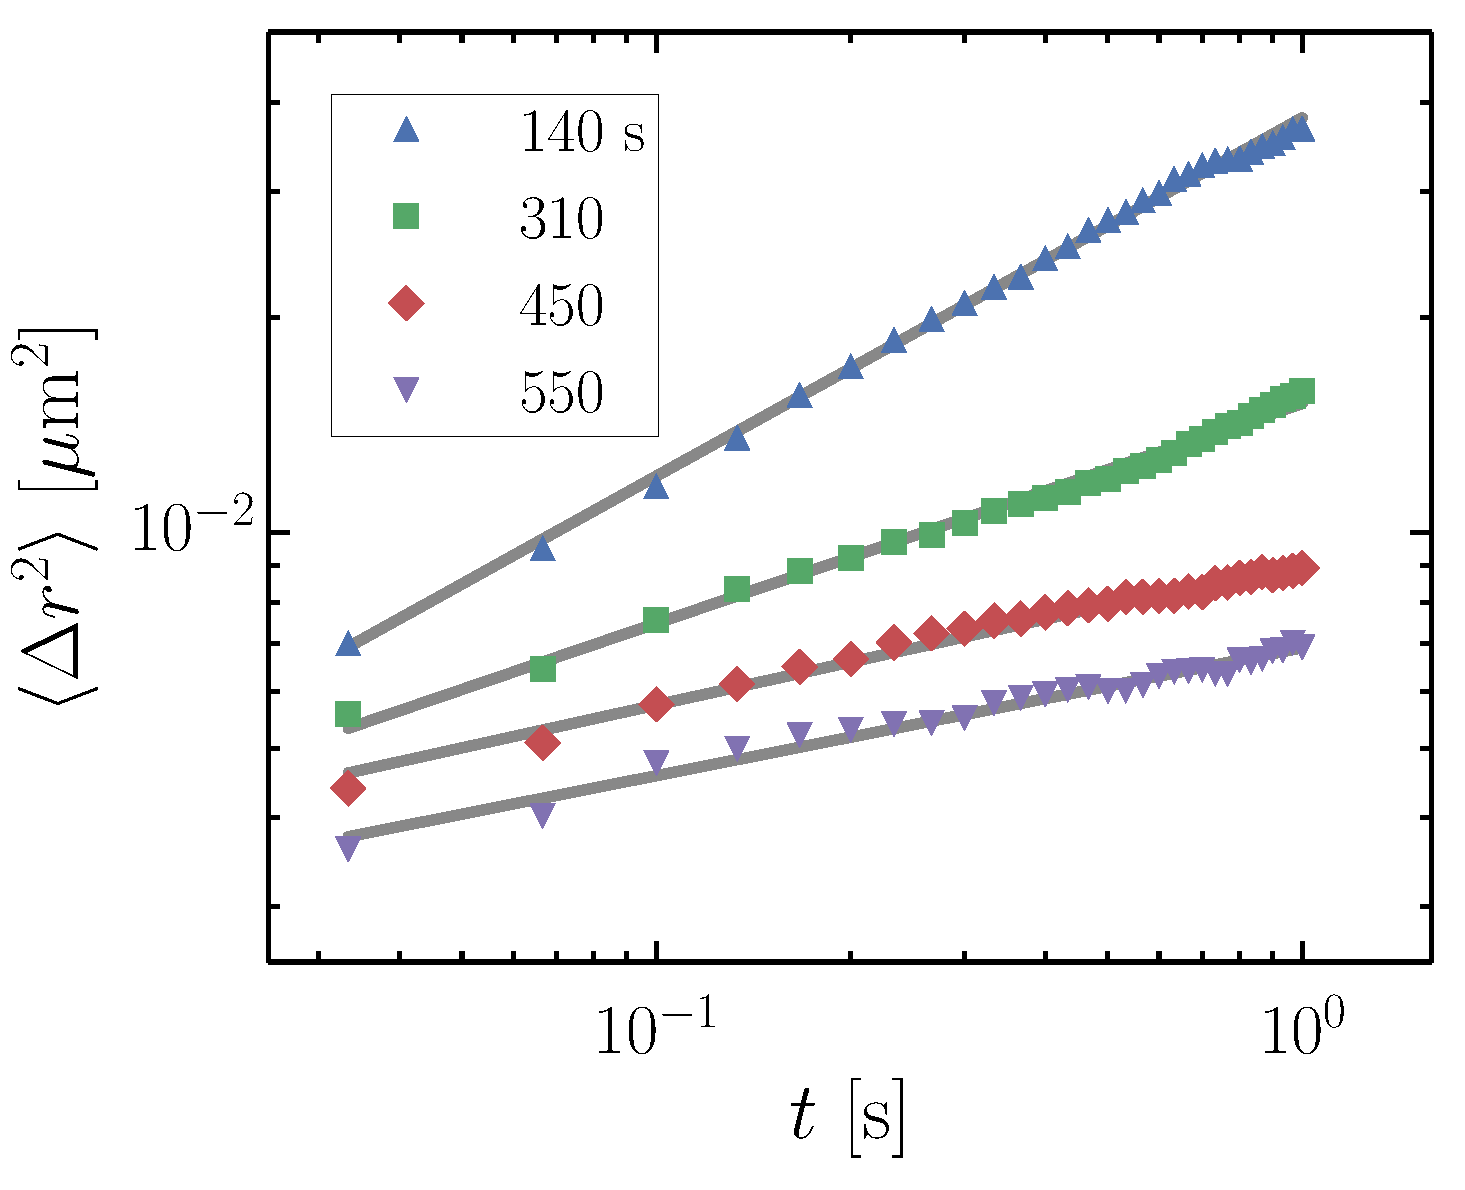
\includegraphics[width=\linewidth,keepaspectratio]{lysozyme/Fig1_msd}
 \caption[\lofimage{lysozyme/Fig1_msd}Ensemble-average mean-squared displacements of colloids at the air interface]{\label{fig:emsds}Ensemble-average mean-squared displacements of 0.5-$\mu$m radius colloids at the air interface of a lysozyme solution (0.05 mg/ml, pH 7.4) at ages $t_a$ = 140 (squares), 310 (diamonds), 450 (triangles), and 550 (solid circles) seconds since formation of the interface.  Also shown is the mean-squared displacement of the probes at the air-buffer interface in the absence of protein.  The solid lines are the results of power-law fits.}
\end{figure}


\begin{figure}
 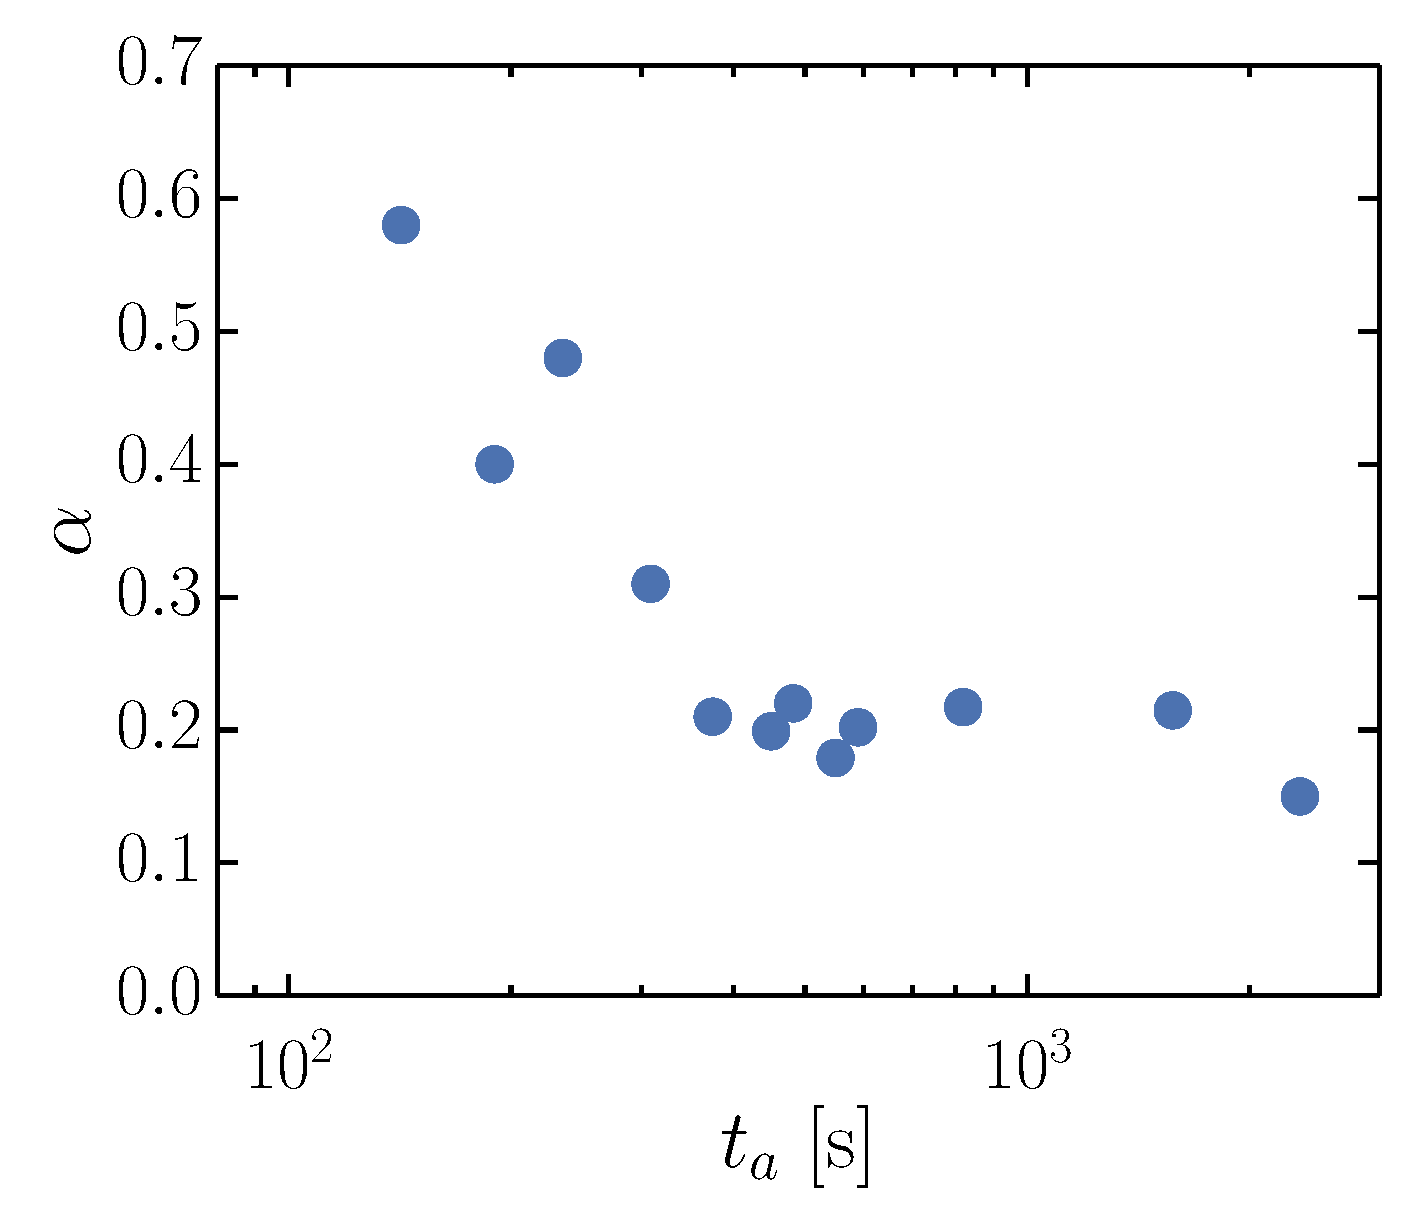
\includegraphics[width=\linewidth,keepaspectratio]{lysozyme/Fig2_power-law-exponent}
 \caption[\lofimage{lysozyme/Fig2_power-law-exponent}Power-law exponent characterizing $\langle \Delta r^2(t) \rangle \propto t^{\alpha}$ as a function of age]{\label{fig:power-law_expon} Power-law exponent characterizing the ensemble average mean-squared displacements, $\langle \Delta r^2(t) \rangle \propto t^{\alpha}$, of colloids at the air interface of a lysozyme solution as a function of the age since formation of the interface.}
\end{figure}

%Such weak power-law frequency dependence is characteristic of the shear rheology of a broad range of complex fluids including concentrated microgel solutions \cite{ketz}, foams \cite{khan}, paint \cite{mackley}, intracellular matrix [Ref], compressed emulsions \cite{mason_colloid},  particulate suspensions, slurries, and liquid-crystal nanocomposites [RanjiniPRL]. In these cases, the power-law exponent typically lies in the range $\alpha \approx$ 0.1 to 0.3.  The soft glassy rheology model~\cite{sollich}, which explains this response as a general consequence of structural disorder and metastability, provides a unifying theoretical framework for this behavior.  In this model, $$ serves as an effective noise temperature, with systems approaching a glass transition as $n \rightarrow 0$.  Thus, the steady decrease in $n$ with layer age seen in Fig.~\ref{fig:power-law_expon} points to increasingly glassy dynamics characterizing the structural response of the lysozyme layer.  Ultimately, at very late ages $\langle \Delta r^2(t) \rangle$ becomes independent of lag time $t$, as illustrated by the results at $t_a$ = ??? minutes in Fig.~\ref{fig:emsds}.  That is, ultimately at very late ages $n \approx 0$.  Thus, such mature lysozyme layers can be considered soft glasses.

%A noteworthy feature of the evolution in probe mobility is the nearly immediate influence of the protein adsorption on the interfacial rheology, as revealed by the onset of subdiffusive behavior, $n \approx 0.6$, less than 3 minutes after layer formation.  This rapid impact of adsorption of lysozyme on the interface  contrasts strongly with layer formation at the air-water interface  of $\beta$-lactoglobulin solutions of similar concentration [LeeLangmuir].  $\beta$-lactoglobulin layers forming at the air-water interface  remain viscous for a protracted period during which the interfacial viscosity increases slowly and undergo a  transition to elastic behavior only at ages of tens of minutes.  This viscoelastic transition is further characterized by pronounced mesoscale heterogeneity in colloidal mobility, where some colloids become localized as if trapped in an elastic film while others continue to undergo diffusion as if in a viscous environment [LeeLangmuir].  We observe no such pronounced heterogeneity in probe mobility at the interface of the lysozyme solutions.  Rather, all probes undergo statistically similar evolution in mobility represented by the ensemble averages in Fig.~\ref{fig:emsds}.  

%The rapid evolution in $\langle \Delta r^2(t) \rangle$ seen in Fig.~\ref{fig:emsds} is more similar to that observed at the oil-water interface of $\beta$-lactoglobulin solutions, where again the onset viscoelastic behavior occurs at a new interface within minutes and no pronounced mesoscale heterogeneity is observed [LeeSoftMatter].  However, more detailed comparison of $\langle \Delta r^2(t) \rangle$ at those interfaces and in the lysozyme layers reveal important differences.  Specifically, evolution in probe mobility in $\beta$-lactoglobulin layers indicated the layers underwent a quasi-two dimensional gel transition, with $\langle \Delta r^2(t) \rangle$ showing characteristics of critical stress relaxation.  In contrast, as mentioned above, we identify the evolving shear rheology of the entry of the layers into a soft glass phase.  We note Cicuta et al. similarly identified layers of $\beta$-lactoglobulin spread on the air-water interface as soft glassy materials [Cicuta].  These different experiments on $\beta$-lactoglobulin and lysozyme together hence indicate that the evolution in the rheology of interfacial protein layers is not universal, and depending on  specific conditions -- such as protein species, hydrophobic phase (e.g., air or oil), and how the protein is introduce onto the interface -- either gel and or glass transitions can underlie the observed viscoelastic transitions.



\subsection{\label{sec:nonlinear}Nonlinear Rheology}

As in the passive microrheology, the active nanowire microrheology reveals a pronounced evolution in the mechanical behavior of the lysozyme layers with increasing layer age.  Close inspection of the results in the active measurements and comparison with those from the passive measurements, however, show that they probe a different aspect of the layer response, specifically its nonlinear rheology.  For example, Figs.~\ref{fig:early-and-late-rotation}(a) and \ref{fig:early-and-late-rotation}(b) display the angle $\theta$ between an 11-$\mu$m-long wire and an applied magnetic field as a function of time following a 90\degree\ step change in the direction of the field at layer ages $t_{\text{a}}=$ 2700 s and 8200 s, respectively.  At early ages, such as $t_{\text{a}}=$ 2700 s (Fig.~\ref{fig:early-and-late-rotation}(a)), the wire rotates rapidly in response to the magnetic torque so that the angle between the wire axis and the magnetic field relaxes fully to zero in a short time, and the response at these ages is consistent with the wire experiencing simple viscous drag.  The dashed line through the data in Fig.~\ref{fig:early-and-late-rotation}(a) shows the result of a fit using the form for viscous drag, Eq.~(\ref{eq:sasha}), which agrees closely with the data.  Such agreement is observed at all layer ages up to $t_a \approx 3000$ seconds.  The interfacial viscosity extracted from the fit using Eq.~(\ref{eq:wire_zeta}) is 21 nPa$\cdot$m$\cdot$s, which implies $L\eta/\eta_s \approx 2$, near the lower limit of interfacial viscosity where Eq.~(\ref{eq:wire_zeta}) is a valid approximation for the drag coefficient. 

\begin{figure}
  \centerline{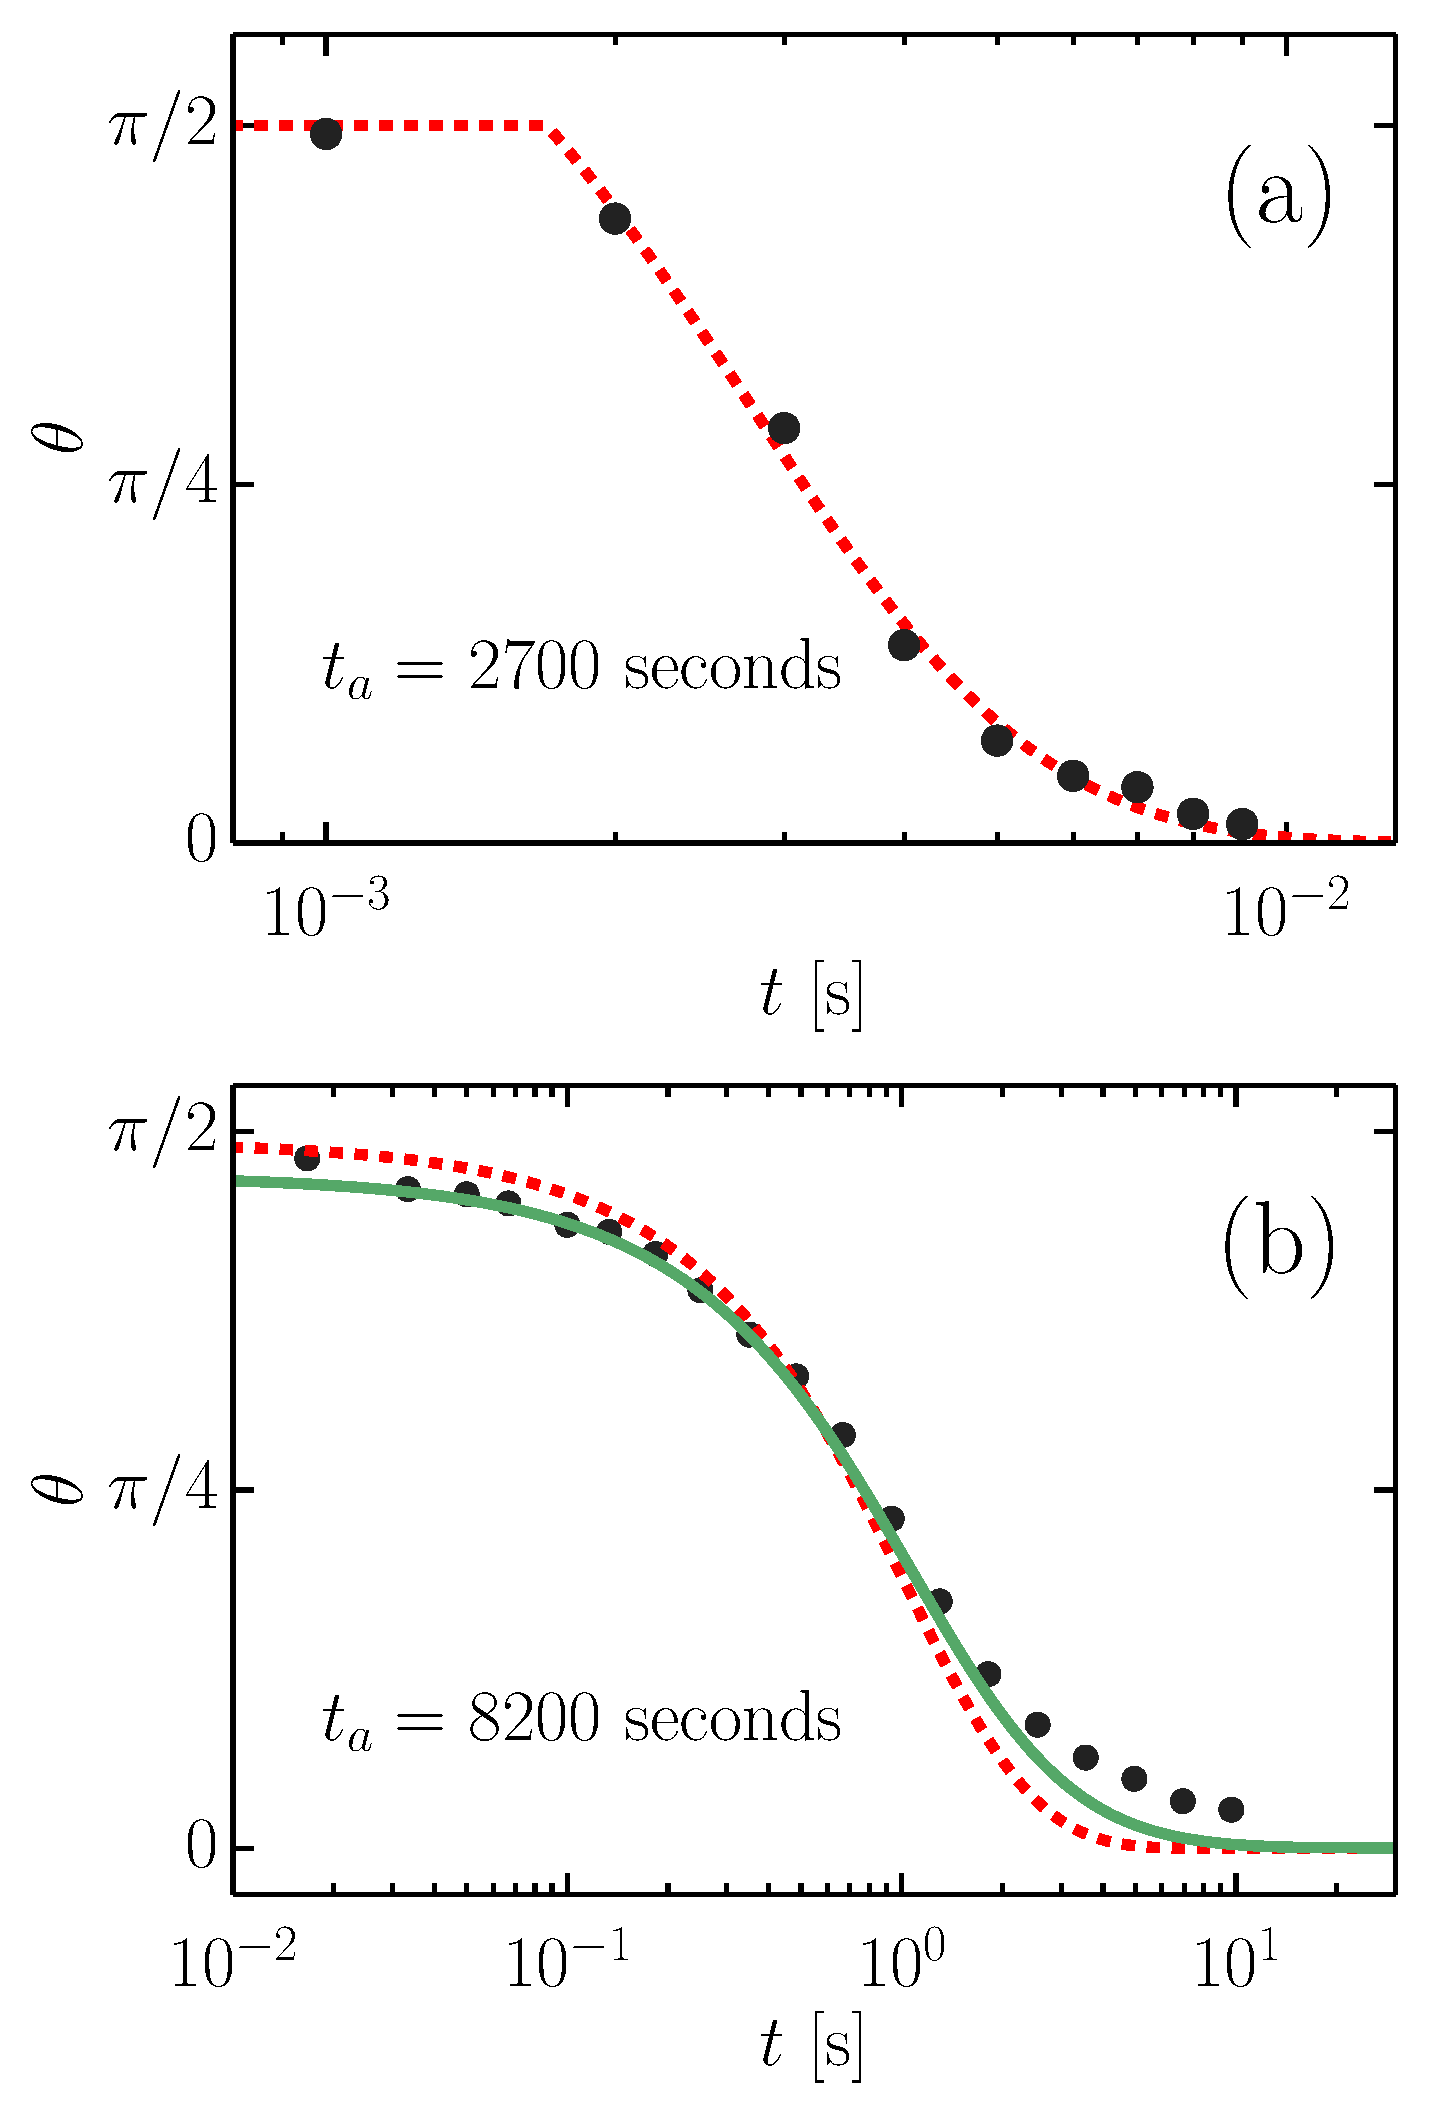
\includegraphics[width=\linewidth,height=0.8\textheight,keepaspectratio]{lysozyme/Fig3_compare-early-late}}
 \caption{\label{fig:early-and-late-rotation} Angle between the axis of a 11-$\mu$m-long Ni nanowire and external magnetic field as a function of time following a step change in the field direction of 90\degree~at interface ages (a) $t_{\text{a}}=$ 2700 s ($B = 30$ G) and (b) $t_{\text{a}}=$ 8200 s ($B = 60$ G).  The dashed lines in (a) and (b) are the results of fits to the data using a form based on simple viscous drag (Eq.~(\ref{eq:sasha})), and the solid line in (b) is the result of a fit using a form based on drag from a power-law fluid (Eq.~(\ref{eq:pf-solution})).}
\end{figure}

Notably, this value of interfacial viscosity, 21 nPa$\cdot$m$\cdot$s, is the same order as that measured previously on $\beta$-lactoglobulin layers at early ages~\cite{Lee2010}.  However, as described in Section~\ref{sec:linear} above, during this span of early ages where the active measurements appear consistent with a viscous layer, the passive measurements show increasingly viscoelastic behavior.  This apparent discrepancy results from the active measurements accessing a nonlinear rheological response from the layers.  Hence, one should not interpret this result as the linear, zero-shear-rate viscosity of the lysozyme layers.  The nonlinear nature of the response is shown clearly in analysis of the nanowire rotation at later ages when the shape of $\theta(t)$ becomes no longer consistent with simple viscous drag.  This change is illustrated by the dashed line in Fig.~\ref{fig:early-and-late-rotation}(b), which shows the result of a fit using Eq.~(\ref{eq:sasha}) to the data at $t_a = 8200$ s and which reveals pronounced deviations of $\theta(t)$ from the viscous lineshape.  Such systematic deviations are apparent in the angular response of the wire at all ages greater than 3000 s.  The solid line through the data in Fig.~\ref{fig:early-and-late-rotation}(b) depicts the result of a fit using the power-law-fluid form, Eq.~(\ref{eq:pf-solution}), to the data with $n \approx 0.6$.  As the fit illustrates, good agreement between the data and Eq.~(\ref{eq:pf-solution}) is found for all ages.  That is, for $t_{\text{a}} < $ 3000 s, best fits with Eq.~(\ref{eq:pf-solution}) give $n \approx 1$ and are indistinguishable from fits with Eq.~(\ref{eq:sasha}), while at later ages $n < 1$, implying shear-thinning behavior.  We note that for shear-thinning power-law fluids, the apparent zero-shear-rate viscosity $\eta_{app}\equiv \sigma/\dot{\gamma} \sim \sigma^{1-1/n}$ diverges in the limit of small shear stress, consistent with the nearly elastic response observed in the passive microrheology at ages greater than 3000 s.

%We note the introduction of the flow index $m$ gives Eq.~(\ref{eq:pf-solution}) one additional free parameter over Eq.~(\ref{eq:sasha}). (QUESTION:  WHAT PARAMETER IN EQ. (7) PLAYS THE ROLE OF $t_0$?)  To provide an alternative comparison between the nonlinear behavior implied by Eq.~(\ref{eq:pf-solution}) and linear viscoelastic behavior, we also include in Fig.~\ref{fig:early-and-late-rotation}(b) the result of a fit of a Maxwell model~\cite{Wilhelm2003} to the data at $t_a = 137$ minutes, shown by the dotted-dashed line. While the inclusion of an elastic component in the layer response improves the agreement over that of strictly viscous drag, the quality of the fit with the Maxwell model is inferior to that with the power-law-fluid model. Thus, the success of Eq.~(\ref{eq:pf-solution}) implies that the nanowire motion probes the nonlinear rheology of the layer.  

While Eq.~(\ref{eq:pf-solution}) describes accurately the angular rotation of the wire through the protein layer, the nonlinear nature of the hypergeometric function makes obtaining stable values for $n$ and $\zeta_{\text{pl}}$ through fits using Eq.~(\ref{eq:pf-solution}) problematic.  However, an alternative approach to modeling the power-law-fluid response is obtained by rearranging the torque balance relation, Eq.~(\ref{eq:pf_wire}), to get
\begin{equation}
\label{eq:pf_linearized}
  \ln(\dot{\theta})= \frac{1}{n}\ln(\sin\theta) + \ln\left(\frac{(\mu B)^{1/n}}{\zeta_{\text{pl}}}\right)
\end{equation}
\noindent Thus, the power-law-fluid model predicts that the logarithm of the time derivative of $\theta(t)$ varies linearly with the logarithm of $\sin\left(\theta\right)$ and that the inverse of the flow index $1/n$ is the proportionality constant.  As a test of this prediction, Fig.~\ref{fig:linearization} shows results for the wire rotation at a series of layer ages plotted in this way, where the values of $\ln(\dot{\theta})$ are obtained from $\theta(t)$ through the Savitzky-Golay smoothing algorithm.~\cite{Savitzky1964}  As the figure indicates, the data follow a linear relationship as expected from Eq.~(\ref{eq:pf_linearized}).~~Further, we find that linear fits with Eq.~(\ref{eq:pf_linearized}) provide a more reliable method of obtaining $n$ than do direct fits to $\theta(t)$ using Eq.~(\ref{eq:pf-solution}).~~For instance, the change from $n \approx 1$ at early ages to shear-thinning behavior at late ages is seen clearly in the change in slope of the data in Fig.~\ref{fig:linearization}.  Figure \ref{fig:m-with-age} displays the values of $n$ extracted from fits using Eq.~(\ref{eq:pf_linearized}) as a function of layer age.  The flow index appears to undergo an abrupt decrease around $t_{\text{a}} = $ 3000 s from $n \approx 1$ to $n \approx 0.7$.  (The data could also be interpreted as a steady decrease in $n$, but one should not expect that $n$ extrapolates at early times to values greater than one, which would imply shear-thickening behavior.)  The values of $n$ obtained for the lysozyme layers at late ages are typical of shear-thinning materials that behave as power-law fluids, where in most cases $0.3 < n < 1$ is observed.~\cite{Huang1998a, Larrard1998}   

\begin{figure}
  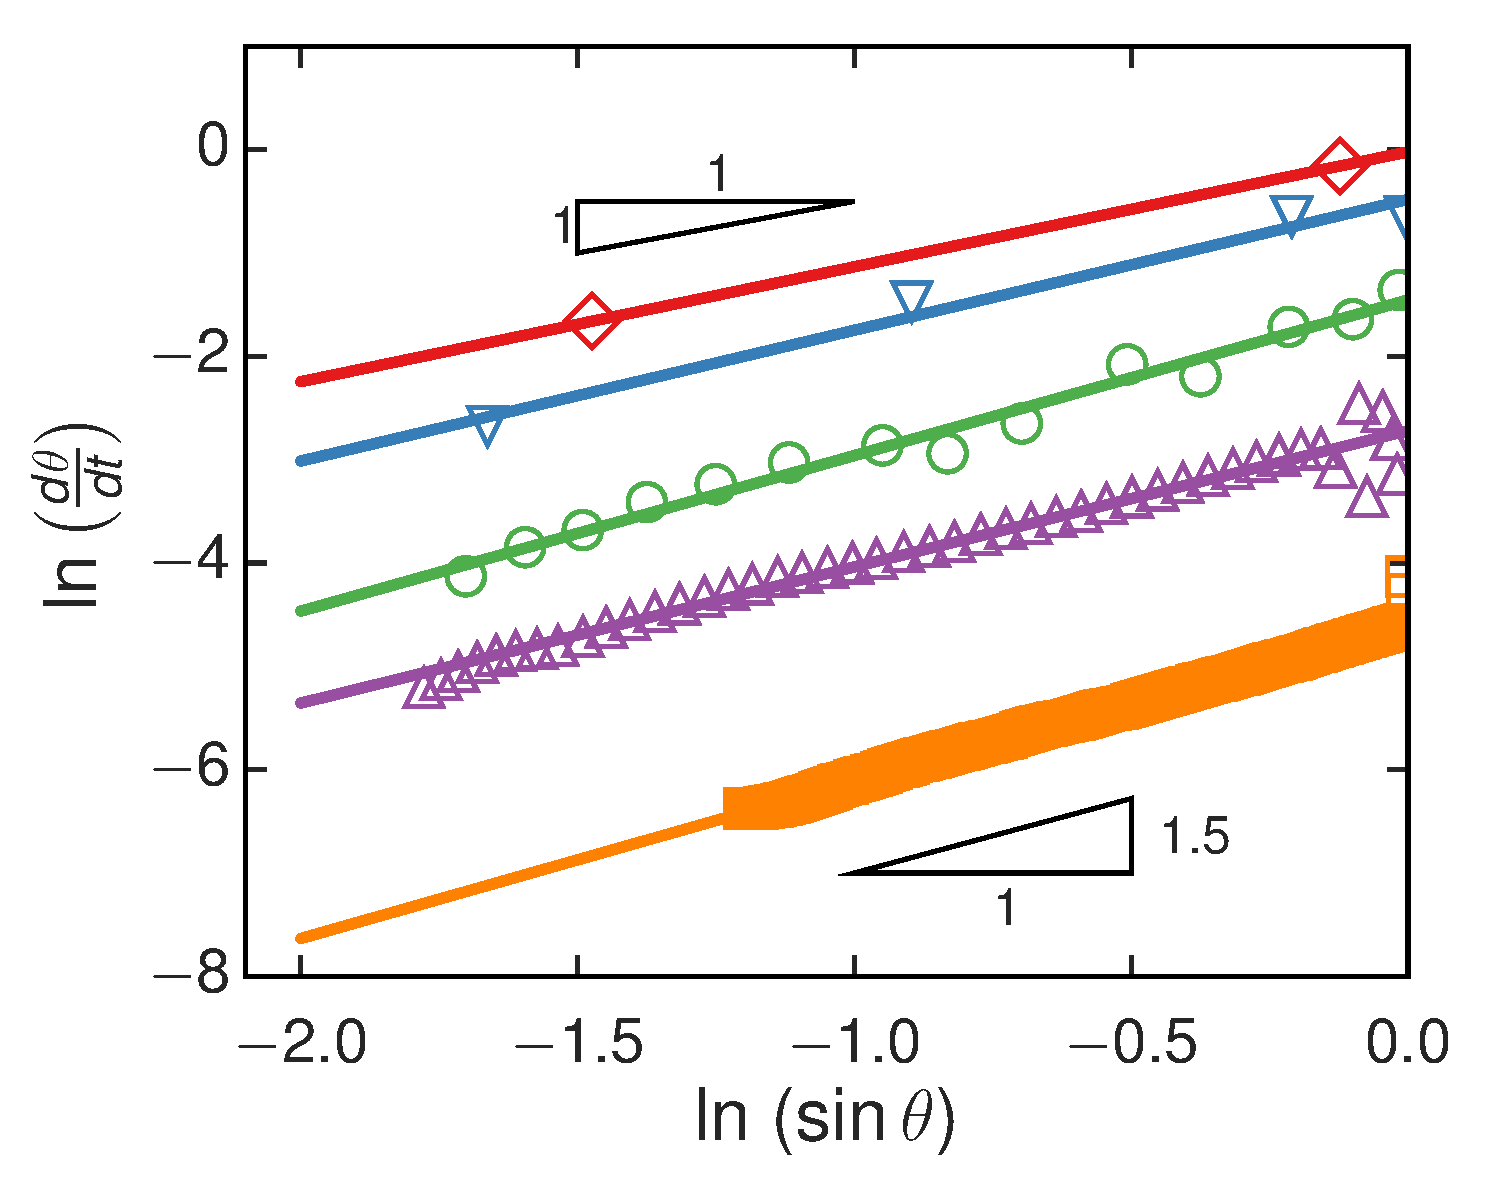
\includegraphics[width=\linewidth,keepaspectratio]{lysozyme/Fig4_linearization-AT20-40G}
 \caption{\label{fig:linearization}  Logarithm of the nanowire rotation rate as a function of the logarithm of $\sin(\theta)$, where $\theta$ is the angle between the wire axis and external magnetic field, at interface ages $t_a =$ 1320 seconds (red circles), 2700 seconds (blue triangles), 3600 seconds (green squares), 5100 seconds (purple diamonds), and 6600 seconds (orange inverted triangles).  The solid lines are the results of linear fits. The slope increases with layer age from near one at early ages to above 1.5 at late ages.}
\end{figure}

%The values of $n$ obtained for the lysozyme layers are typical of shear-thinning materials that behave as power-law fluds, where in most cases $0.3 < n < 1$ is observed [Huang1998a, Larrard1998].  
%Notably, the soft glassy rheology model, which as described above predicts weak power-law frequency dependence in the linear shear modulus $G^*(\omega)$ in disordered soft materials, also predicts power-law fluid behavior in the nonlinear rheology of these materials.  Further, according to the model the flow index increases on approaching the glass transition.  Thus, qualitatively the linear and nonlinear responses of the lysozyme layers fit well together as those of a soft glassy material that approaches a glass phase with increasing age.  [Footnote here noting that according to SGR power-law-fluid $n$ is equal to $n$ from MSD fit, which we don't see, but does anybody?]. 


\begin{figure}
  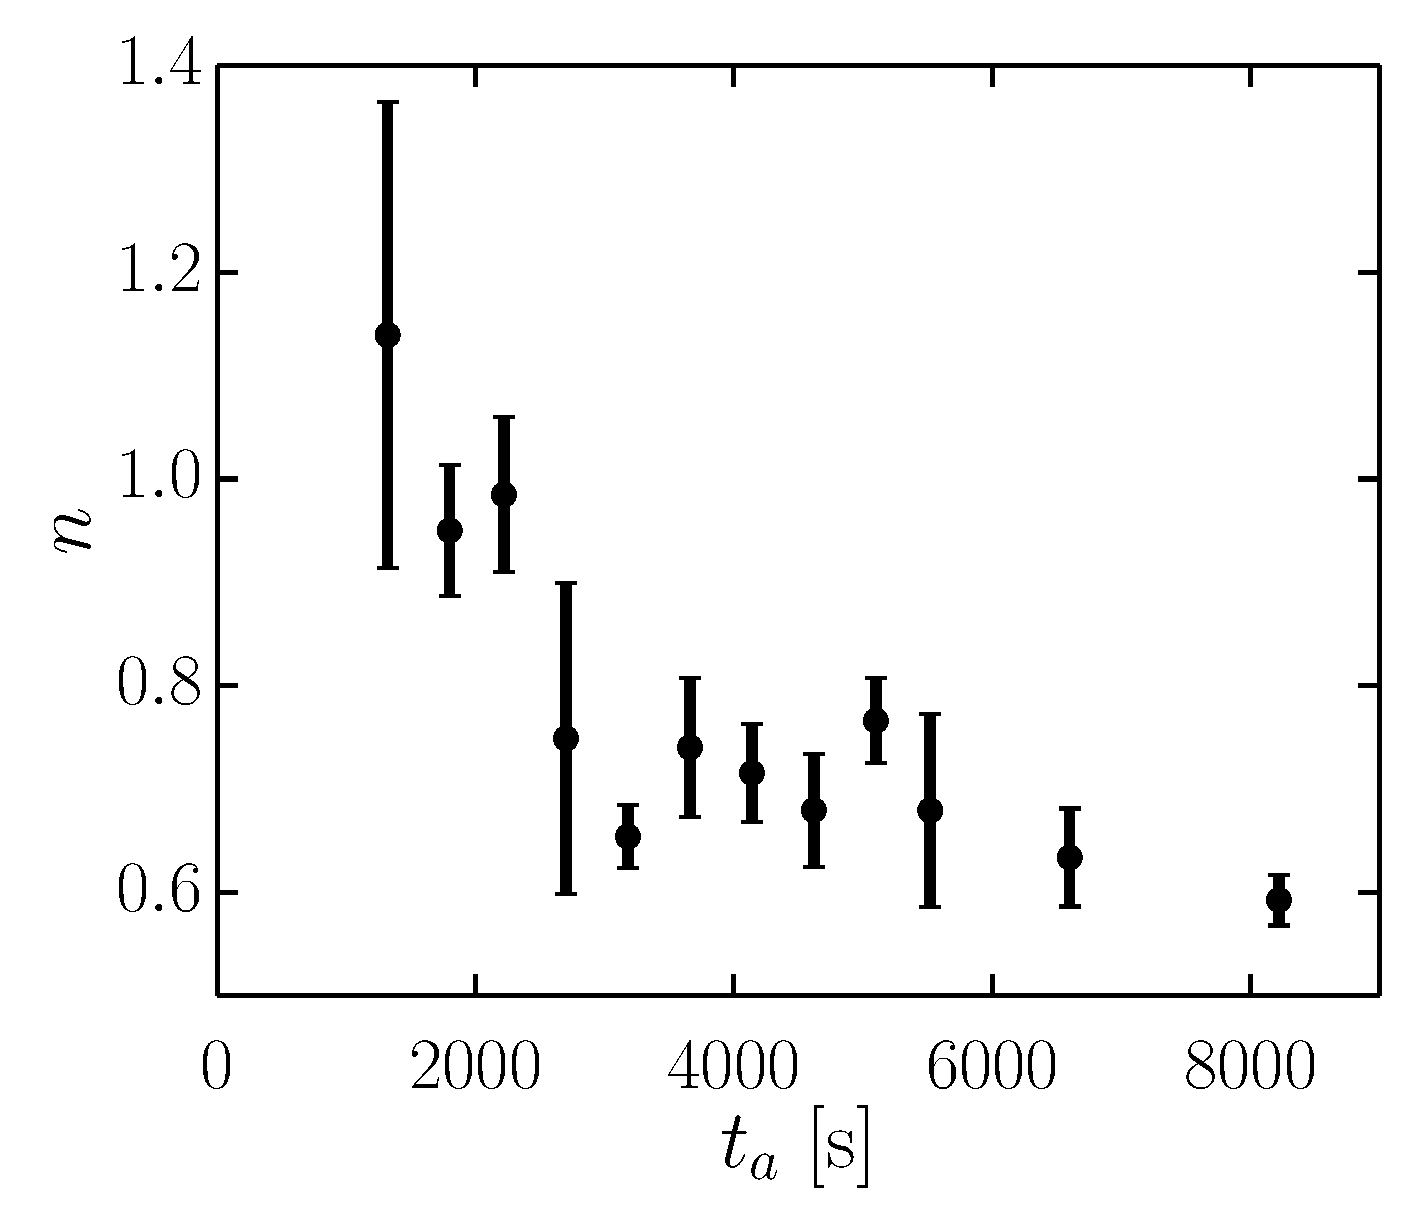
\includegraphics[width=\linewidth,keepaspectratio]{lysozyme/Fig5_m-with-age-avg-fields}
  \caption{\label{fig:m-with-age}Flow index $n$ as a function of layer age. At each age, $n$ is determined from measurements at several magnetic-field values. The error bars incorporate both statistical variation in $n$ and measurement uncertainty.}
\end{figure}


%Applying the re-parameterization to a trial with known purely viscous behavior returned the desired parameter m = 1, and the intercept b was found to decrease with age, as shown in Fig.~(\ref{fig:linearized-AT32}). These results are consistent with an increasing viscosity, though the technical limitations of both the Savitzky-Golay smoothing at sharp derivatives and the logrithmic convolution at shallow derivates prevents accurate extraction of $\zeta_{\text{pl}}$ beyond an order of magnitude. However, extraction of m values through re-parameterization was found to be both robust and reproducable, and ranged from 1 in viscous cases to ~3 for late age samples, consistant with results from direct fitting to the power-law model (Figure here of late age AT20 and AT21).

%The main utility of linear reparameterization is to verify the non-newtonian, power-law behavior of the interfacial layer, and to provide an accurate value of m for use in direct fitting of the analytical solution. 

\begin{figure}
 \centerline{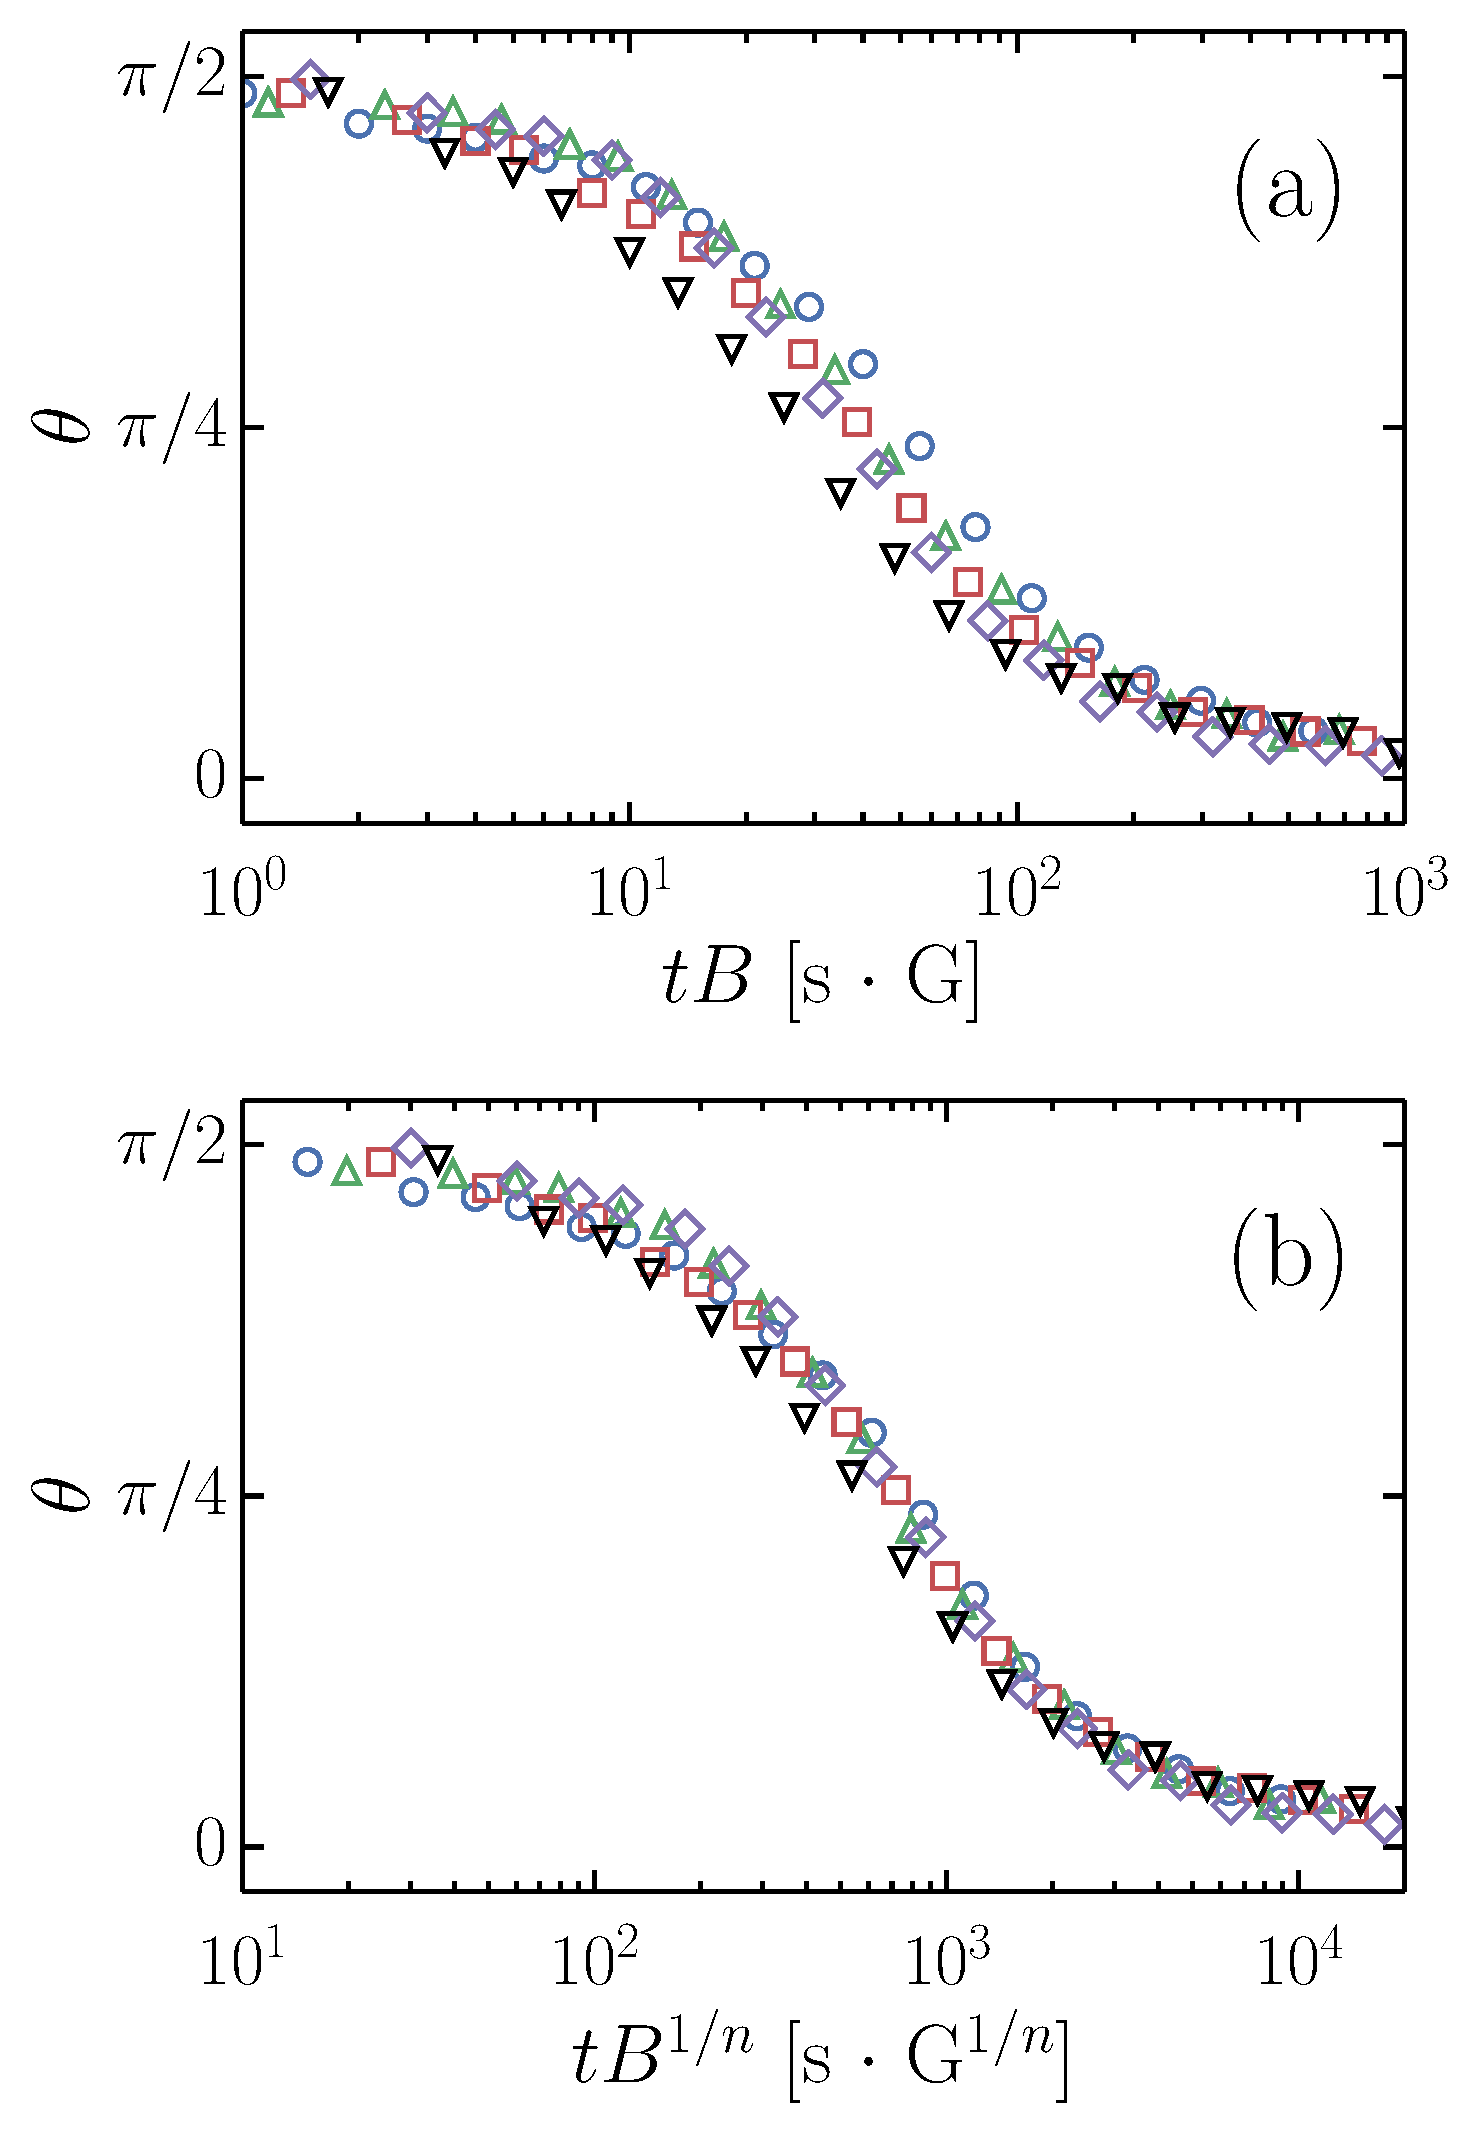
\includegraphics[width=\linewidth,height=0.8\textheight,keepaspectratio]{lysozyme/Fig6_rescaled-curves-137}}
 \caption{\label{fig:scaling}Angle between wire and magnetic field as a function of time scaled by magnetic field strength $B$ for field strengths of 60 (circle), 70 (triangle), 80 (square), 90 (diamond), and 100 G (inverted triangle).  In (a) time is scaled linearly with field strength; in (b) time is scaled by $B^{1/n}$ with $n=0.6$, the value obtained from fits to $\theta(t)$. The interface age is $t_a = 8200$ seconds.}
\end{figure}

While the success of Eqs.~(\ref{eq:pf-solution}) and (\ref{eq:pf_linearized}) provides strong evidence that the layer response in the active microrheology experiments reflects the nonlinear rheology, this nonlinear behavior is more directly demonstrated in the dependence of the wire rotation rate on the magnetic-field strength $B$.  Since the torque on the wire is proportional to $B$, a viscous-like linear response from the layer should lead to a rotation rate that is similarly proportional to $B$.  Figure \ref{fig:scaling}(a) shows results for the rotation angle from a set of measurements at $t_a = 8200$ s at various field strengths with time scaled by $B$.  In contrast to the expectations of linear response, the curves at different $B$ fail to collapse.  Better scaling is achieved assuming the nonlinear relation between rotation rate and $B$ implied by the power-law-fluid form of Eq.~(\ref{eq:pf_wire}), as shown in Fig.~\ref{fig:scaling}(b).

A common property of the rheology of shear-thinning, thixotropic materials is a recovery period following application of a nonlinear stress during which the shear-altered structure relaxes back to its quiescent state.  We searched for such effects in the active microrheology on the lysozyme layers by varying the waiting time between wire rotations and by varying the sequence of magnetic field values.   We found no discernible transient behavior for waiting times as small as 2 seconds, the minimum we could access experimentally.

Another key feature of the protein-layer response in the active microrheology is the steady evolution of the timescale of the response as the layer ages.  This evolution is characterized by the dependence of the power-law drag coefficient $\zeta_{pl}$ on layer age, as shown in Fig.~\ref{fig:zeta-powerlaw}.  Because the dimensionality of $\zeta_{pl}$ depends in $n$, for consistency Fig.~\ref{fig:zeta-powerlaw} shows values obtained by fitting $\theta(t)$ at different ages using Eq.~(\ref{eq:pf-solution}) with the flow index fixed at $n=0.70$, its average at ages $t_a > 3000$ s.  As Fig.~\ref{fig:zeta-powerlaw} indicates, $\zeta_{pl}$ grows approximately exponentially, implying a dramatic slowing of the layer response with increasing age. This trend is insensitive to the precise value of $n$ used to obtain $\zeta_{pl}$.  This quasi-exponential increase in the drag is very similar to the behavior seen in earlier studies employing nanowires in active microrheology of protein layers formed from $\beta$-lactoglobulin and albumin.~\cite{Lee2010, Dhar2010}  In those earlier studies, the angular motion was analyzed using a form equivalent to Eq.~(\ref{eq:sasha}), thus assuming a simple viscous response.  However, even in those cases, evidence suggested the nanowire microrheology was accessing nonlinear properties of the layer rheology.~\cite{Lee2010}  Here, the nonlinear nature of the response is seen clearly in the values of the flow index $n$ at late ages and in the nonlinear scaling in Fig.~\ref{fig:scaling}(b).  We note that we repeated the active microrheology measurements on lysozyme layers several times and found that, while an evolution to shear thinning like that depicted in Fig.~\ref{fig:m-with-age} was reproducible, the precise values of $n$ at late ages varied between trials, and we observed instances of layer formation in which the response remained essentially viscous-like ($n \approx 1$), with a viscosity that rose dramatically with age much like $\zeta_{pl}$ in Fig.~\ref{fig:zeta-powerlaw}. While we do not have a firm explanation for this variation in $n$ between trials, we believe these observations support the conclusion that the response shown by the lysozyme layers and those reported previously for $\beta$-lactoglobulin and albumin share the same basic features of nonlinear behavior characteristic of power-law fluids.  


\begin{figure}
  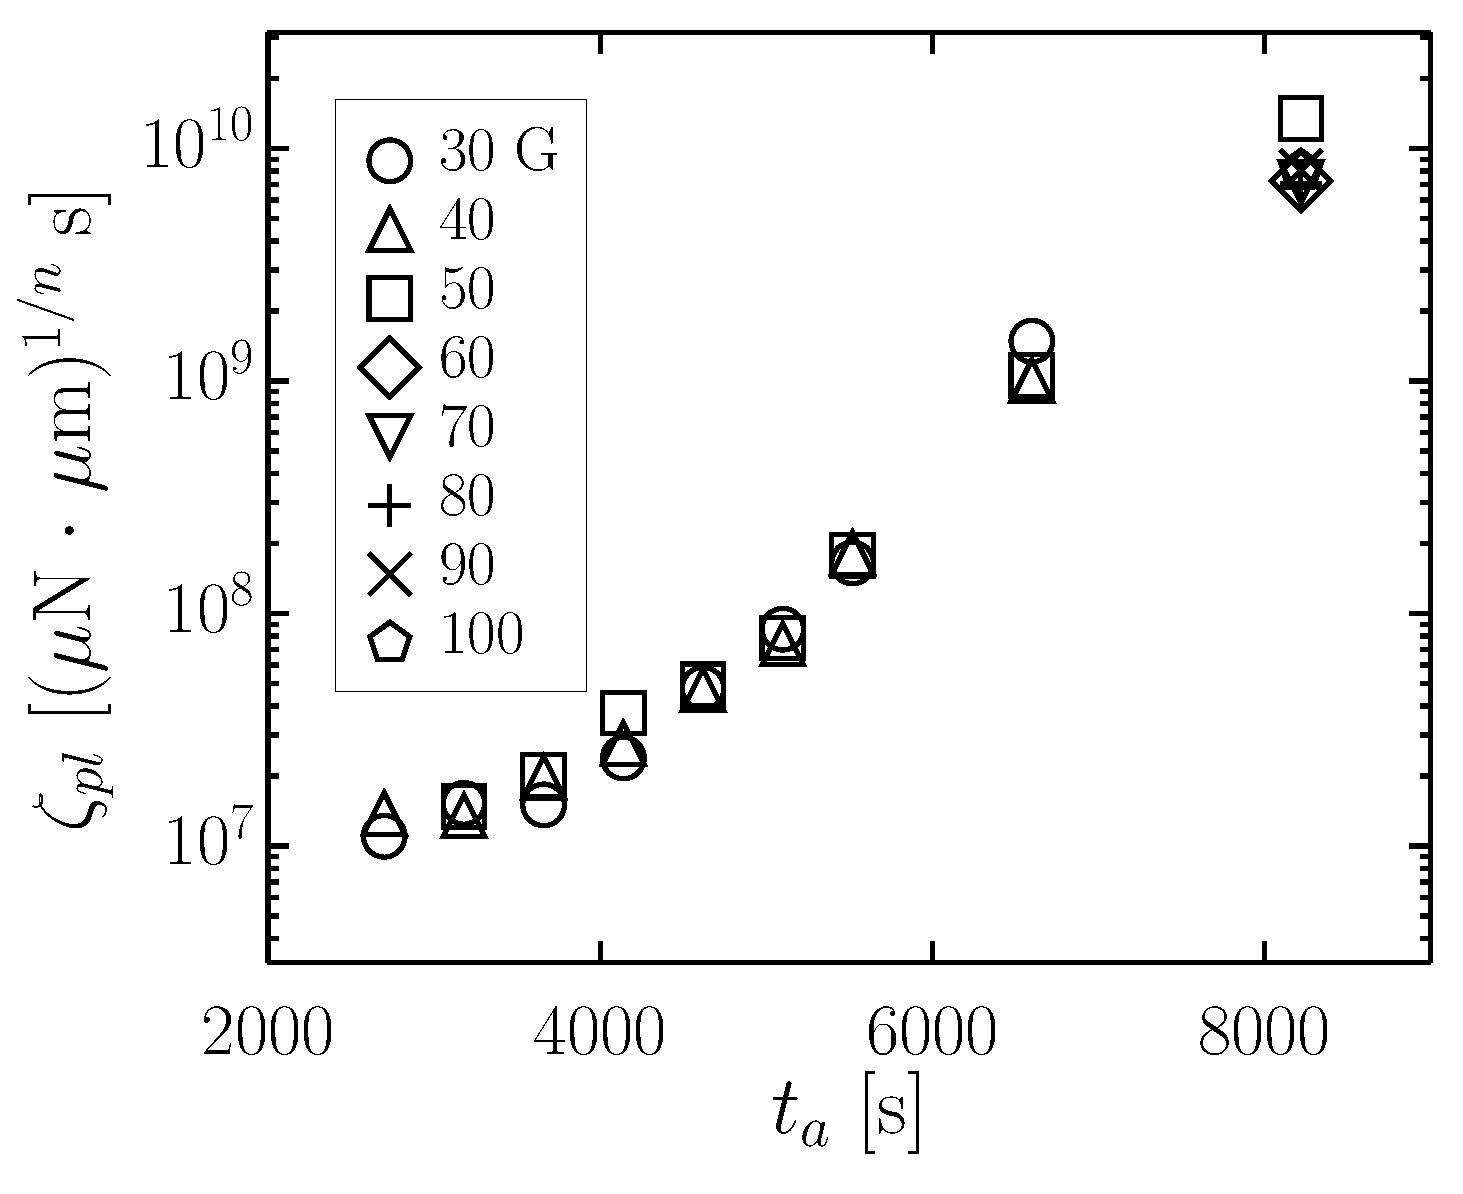
\includegraphics[width=\linewidth,keepaspectratio]{lysozyme/Fig7_zeta-powerlaw}
  \caption{\label{fig:zeta-powerlaw}Power-law drag coefficient $\zeta_{pl}$ as a function of interface age. Values are obtained at a range of field strengths as indicated in the legend and are determined from fits using Eq.~(\ref{eq:pf-solution}) with the flow index fixed at $n = 0.70$, the average value at ages $t_a > 3000$ s.}
\end{figure}

%(Linear reparameterization of the form given in Eq.~(\ref{eq:pf_linearized}) was also applied to films that displayed known Maxwell like viscoelasticity, and a characteristic upward curvature was found in the limit $ln\left(sin\left(\beta - \theta\right)\right)\rightarrow{0}$. This characteristic feature of a Maxwell film was not observed in any trial on lysozyme films.)

%We note the power-law fluid behavior in the nonlinear response persists to very late ages ($t_a > 120$ minutes), when the passive microrheology shows a constant $\langle r^(t) \rangle$ implying an elastic layer with frequeny-indepenent shear modulus.  As mentioned above, within the soft glassy rheology model, this elasticity implies the layer has become a soft glass.  The model further predicts that materials inth  glass phase behave as Herschel–-Bulkley fluids, with a power-law fluid response to stress above a critical yield stress as in Eq.~(\ref{eq:HB}).~~Therefore, an interesting question about the layers' non-Newtonian rheology at very late ages is whether it is precisely that of a power-law fluid or whether the layers possess some small yield stress.  Evidence opposing the existence of any yield stress comes from the linear dependence of $\ln(\dot{\theta})$ on $\ln(\sin\theta)$ in Fig.~\ref{fig:linearization}. The presence of a yield stress would lead to upward curvature on such plots.  Fitting the results at late age using a Hershel-Bulkley form, we can place an upper bound on the yield stress of ???.  In addition, the wires display no measurable recoil when the external field is removed, indicating no stored elastic deformation.   However, as noted above we also observed some variability in the layer response in the active microrheology, both for different trials and for different wires within a single layer, and in some cases wire motion became imperceptible at very late layer ages, and we are unable to distinguish this immobility as the onset of rigidly and or as extremely large $\zeta_{pl}$.  
%Further, additional experiments probing layer formation at the air interface of lysozyme solutions with very low bulk protein concentrations (below 0.01 mg/ml) suggested the adsorb protein associates to form a rigid network.  At these low concentrations, which are inadequate to provide full coverage of the interface through adsorption, we observed wires to rotating off-center, as if partially trapped in an rigid ``island'' of protein.  
%Another property predicted by the soft glassy rheology model for the glass phase is nonergodicity and aging behavior.  One interpretation for the growth in $\zeta_{pl}$ in Fig.~\ref{fig:zeta-powerlaw} is that it reflects physical aging.  However, we believe the growth in $\zeta_{pl}$ stems from other factors.  Aging is usually manifest as a power-law growth in relaxation times with age, not the much stronger exponential growth seen in $\zeta_{pl}$.  A number of changes to the layer such as growing protein concentration, slowly changing protein conformations, and protein-protein association could underlie the growth in $\zeta_{pl}$.

%To understand better the nature of the non-Newtonian response of the layer to the rotating wire, we performed experiments to image the flow field around a wire by spreading spherical colloids and wires together at an interface of a lysozyme solution. After allowing an interfacial layer to form ($t_a$ = 140 minutes), we applied a rotating 100 G field to spin the wires at an angular frequency of 0.5 Hz.  Colloids in the vicinity of each wire served as tracers of the resulting flow around the wire, following circular trajectories as illustrated in Fig.~\ref{fig:wire-flow-field}, which shows an image of spheres along with their trajectories in the vicinity of ?? $\mu$m wire.  Figure~\ref{fig:tangential-velocity} displays the tangential velocity $v$ of the spheres as a function of their radial distance $r$ from the center of the wire.  The velocity decreases approximately inversely with distance, $v \sim 1/r$.  Such $1/r$ dependence is a character of two-dimensional Stokes flow around a rotating body.  Thus, surprisingly, the shear thinning does not measurably alter the flow profile.  (Is this really surprising?  DAN: What was $m$ at the time this measurement was made??  If $m \approx 1$ maybe we should remove this paragraph.)



%\begin{figure}
 %\includegraphics[width=\linewidth,keepaspectratio][\linewidth,keepaspectratio]{graphics/rising-viscosity-AT32}
% \caption{\label{fig:linearized-AT32}In this trial, a 0.1 mg/ml protein solution remained purely viscous in the region observed, with a viscosity that rose steadily with age, indicating increased $\zeta_{\text{pl}}$. Viscosities were extracted using fits to the form Eq.~(\ref{eq:sasha})}
%\end{figure}

%\begin{figure}
%  \includegraphics[width=\linewidth,keepaspectratio][\linewidth, keepaspectratio]{graphics/wire-flow-field}
%  \caption{\label{fig:wire-flow-field}Colored lines trace the trajectories of passive colloidal spheres in the vicinity of a rotating wire.}
%\end{figure}

%\begin{figure}
%  \includegraphics[width=\linewidth,keepaspectratio][\linewidth, keepaspectratio]{graphics/tangential-velocity}
%  \caption{\label{fig:tangential-velocity}The tangential velocity $v$ of colloids varied with their distance $r$ from the center of the wire rotating at 100 Hz. The line is a best fit to power-law, which gives the dependence $v \propto 1/r^{1.08}$}
%\end{figure}

\section{\label{sec:discussion}Discussion}

\subsection{Nature of the Viscoelastic Transition}

The linear and nonlinear rheology of lysozyme layers revealed by the passive and active microrheology, respectively, provide a coherent picture of the layers' viscoelastic transition.  In this section, we discuss two frameworks in which to interpret this transition:  the formation of a soft glass phase and critical behavior associated with gelation.  These two frameworks, while not entirely mutually exclusive, imply different possible microscopic mechanisms driving the viscoelasticity.  As discussed in Section \ref{sec:background} above, reflectivity and spectroscopy studies of lysozyme layers have led to a debate about the degree that lysozyme unfolds upon adsorption.  Since the intermolecular interactions at the interface will depend on conformation, understanding the microscopic origin of the viscoelastic behavior of the layers can potentially contribute to this debate.  As discussed below, both frameworks are successful in accounting for some but not all aspects of the observed evolution in shear rheology.  

\subsubsection{Soft Glassy Rheology Model}~Weak power-law frequency dependence of $G^*(\omega)$, like that implied by the power-law growth in $\langle \Delta r^2(t) \rangle$, is characteristic of the rheology of a broad range of disordered complex fluids including concentrated microgel solutions,~\cite{Ketz1988} foams,~\cite{Khan1988} paint,~\cite{Mackley1994} intracellular matrix,~\cite{Fabry2001} compressed emulsions,~\cite{Mason1995}  clay suspensions,~\cite{Bonn2002} and liquid-crystal nanocomposites. \cite{Bandyopadhyay2005}   In most cases, the power-law exponent typically lies in the range $\alpha \approx$ 0.1 to 0.3.  The soft glassy rheology model,\cite{Sollich1998} which explains this response as a general consequence of structural disorder and metastability, provides a unifying theoretical framework for this behavior.  Cicuta {\it et al.} have identified layers of $\beta$-lactoglobulin spread on the air-water interface as such soft glassy materials.\cite{Cicuta2003}  Significantly, no specific interparticle associations are required to form soft glassy phases, and purely repulsive interactions within a crowded interface would be sufficient.  Thus, the picture of lysozyme layers as soft glasses is consistent with the protein retaining its native conformation upon adsorption.  In the model, $\alpha$ serves as an effective noise temperature, with systems approaching a glass transition as $\alpha \rightarrow 0$.  Thus, within this picture the steady decrease in $\alpha$ with layer age seen in Fig.~\ref{fig:power-law_expon} points to increasingly glassy dynamics characterizing the structural response of the lysozyme layers.  Notably, the soft glassy rhoelogy model also predicts power-law fluid behavior in the nonlinear rheology of these materials.  Further, according to the model the flow index decreases on approaching the glass transition.  Thus, the linear and nonlinear responses of the lysozyme layers qualitatively fit well together as those of a soft glassy material that approaches a glass phase with increasing age.  More quantitatively, however, the soft glassy rheology model predicts a specific relation between the linear rheology and power-law fluid response,  $n = \alpha$.  The lysozyme layers violate this relation.  This violation suggests that, while the model captures many essential features of the observed mechanical response of the layers, the relationship between structural relaxation and flow in the disordered layers is perhaps more complicated than is assumed in the model.

\subsubsection{Critical Behavior of Gelation}~Materials exhibiting critical stress relaxation on approaching a gel point similarly display weak power-law frequency dependence of $G^*(\omega)$.\cite{Winter1986}  Technically, power-law behavior over an arbitrarily extended range occurs only at the critical point, and at low frequencies (large lag times) the rheology crosses over from viscous-like to elastic as the gel formation progresses.\cite{Winter1986,Veerman2006}  Nevertheless, over a limited dynamic range like that in the passive microrheology measurements, this behavior can appear as a quasi-power law in the mean-squared displacement, $\langle \Delta r^2(t) \rangle \sim t^{\alpha}$, with a power-law exponent that decreases steadily with age.   Indeed, the age-dependent $\langle \Delta r^2(t) \rangle$ in Fig.~\ref{fig:emsds} appear strikingly similar to those obtained in microrheology studies of bulk peptide and polymer solutions undergoing three-dimensional critical gelation.\cite{Veerman2006,Larsen2008}  Identifying the viscoelastic transition in the lysozyme layers with gel formation implies intermolecular bonding capable of creating a percolating network.  The stability of native lysozyme against aggregation in bulk solution suggests that such bonding would require significant unfolding to proceed.  However, anecdotal evidence indicating the adsorbed protein indeed associates to form a network comes from additional active microrheology experiments at the air interface of lysozyme solutions with very low bulk protein concentrations (below 0.01 mg/ml).  At these low concentrations, which are inadequate to provide full coverage of the interface through adsorption, we observed wires to rotate off-center, as if partially trapped in an ``island'' of protein that would form only through attractive interactions.  

\subsubsection{Possibility of a Yield Stress at Late Ages}~An interesting question is whether the lysozyme layers at very late ages display a yield stress in the microrheology measurements.  According to the soft glassy rheology model, the soft glass phase has elastic linear rheology, $\alpha = 0$, and a nonlinear response characteristic of a Herschel-Bulkley fluid as in Eq.~(\ref{eq:HB}).   Similarly, a gel phase would display a yield stress.  While a decrease in $\alpha$ with layer age like that in Fig.~\ref{fig:power-law_expon} was reproducible in the passive microrheology experiments, the final value of $\alpha$ varied from trial to trial, and in some cases the data at late ages was consistent with $\alpha \approx 0$.  Similarly, we also observed some variability in the layer response in the active microrheology, both for different trials and for different wires within a single layer (which we attributed to heterogeneity in the layers), and in some cases wire motion in response to the magnetic torque became imperceptible at late layer ages.  However, we were unable to distinguish this immobility as the onset of rigidity and or as an extremely large $\zeta_{pl}$, and in no cases could we say for certain that the lysozyme layers acquired a yield stress.  For example, evidence opposing the existence of any yield stress comes from the linear dependence of $\ln(\dot{\theta})$ on $\ln(\sin\theta)$ in Fig.~\ref{fig:linearization}. The presence of a yield stress would lead to upward curvature on such plots.  Fitting to the data at late age using a Hershel-Bulkley form gives a result consistent with zero yield stress and allows us to place an upper bound on the yield stress of $\sim 5 \mu$N/m.  In addition, wires in layers at late age rotated fully through $\pi/2$ (when they turned at all) and displayed no measurable recoil when the external field was removed, indicating no stored elastic deformation.   

%Another property predicted by the soft glassy rheology model for the glass phase is nonergodicity and physical aging.  One interpretation for the growth in $\zeta_{pl}$ in Fig.~\ref{fig:zeta-powerlaw} is that it reflects physical aging.  However, we believe this growth in $\zeta_{pl}$ stems primarily from other factors.  First, physical aging is usually manifest as a power-law growth in relaxation times with age, in contrast to the much stronger exponential growth seen in $\zeta_{pl}$.  Also, a number of other possible changes in the layer with age -- such as growing protein concentration, slowly changing protein conformations, and protein-protein association -- could influence the evolution in rheology and underlie the growth in $\zeta_{pl}$.

\subsection{Comparison with Other Protein Layers}

A noteworthy feature of the evolution in probe mobility in the passive measurements is the nearly immediate influence of the protein adsorption on the interfacial rheology, as revealed by the onset of subdiffusive behavior, $\alpha \approx 0.6$, less than 200 seconds after interface formation.  This rapid impact of adsorption of lysozyme on the interface  contrasts strongly with layer formation seen at the air-water interface  of $\beta$-lactoglobulin solutions of similar concentration.~\cite{Lee2010}  $\beta$-lactoglobulin layers forming at the air-water interface  remain viscous for a protracted period during which the interfacial viscosity increases slowly and undergo a  transition to elastic behavior only at ages of tens of minutes.  This viscoelastic transition is further characterized by pronounced mesoscale heterogeneity in colloidal mobility, where some colloids become localized as if trapped in an elastic film while others continue to undergo diffusion as if in a viscous environment.~\cite{Lee2010}  We observe no such pronounced heterogeneity in probe mobility at the interface of the lysozyme solutions.  Rather, all probes undergo statistically similar evolution in mobility represented by the ensemble averages in Fig.~\ref{fig:emsds}.  The rapid evolution in $\langle \Delta r^2(t) \rangle$ seen in Fig.~\ref{fig:emsds} is more similar to that observed at the oil-water interface of $\beta$-lactoglobulin solutions, where again the onset viscoelastic behavior occurs at a new interface within minutes and no pronounced mesoscale heterogeneity is observed.~\cite{Lee2011}  
%However, more detailed comparison of $\langle \Delta r^2(t) \rangle$ at those interfaces and in the lysozyme layers reveals important differences.  Specifically, the evolution in probe mobility in the $\beta$-lactoglobulin layers at the oil-water interface indicated the layers underwent a quasi-two dimensional gel transition, with $\langle \Delta r^2(t) \rangle$ showing characteristics of critical stress relaxation.  In contrast, as described above, we identify the evolving shear rheology of the lysozyme layers with the entry of the layers into a soft glass phase.  
These different experiments on $\beta$-lactoglobulin and lysozyme taken together hence indicate that the evolution in the rheology of interfacial protein layers is not universal, and that depending on  specific conditions---such as protein species, hydrophobic phase (air or oil), and how the protein is introduce onto the interface--- the viscoelastic transitions can proceed through different scenarios.  

\section{\label{sec:conclusion}Conclusion}

In summary, these microrheology experiments tracking the evolution of the air-water interface during lysozyme adsorption have elucidated the linear and nonlinear properties of the viscoelastic transition that the interfacial protein layer undergoes.  As discussed above, interpreting the nature of this transition can contribute to our understanding of the dominant molecular-scale interactions involved in protein-layer formation.  In our analysis of the viscoelasticity of the lysozyme layers, we considered two frameworks for interpretation:  gelation and the formation to a soft glassy phase.  Further microrheology studies that can distinguish more conclusively between these possibilities would be valuable.   Indeed, a key challenge in the field of disordered soft materials is to correlate microstructural properties with the broad distribution of slow relaxation times that give rise to their characteristic rheology.  The quasi-two-dimensional geometry of the layers lends itself to experimental approaches that are unavailable in bulk systems.  For example, experiments comparing imaging with surface pressure have provided insight into layer formation,\cite{Erickson2000} and correlating the results of such experiments with microrheology could provide important new information.  However, another clear conclusion from the microrheology is the sensitivity of the viscoelastic properties of the layers to the specific conditions under which the proteins encounter and associate with the interface.  Hence, any studies comparing rheology with surface structure, surface pressure, other properties would need to take particular care to achieve identical conditions for valid comparisons.

%\section{Appendix}

%We can simplify $_2\text{F}_1(a, b, c; z)$ by exploiting the simple relationship between arguments $b$ and $c$. In general

%\begin{equation}
%  _2\text{F}_1(a, b, c; z) = 
%  \sum\limits_{k=0}^\infty\frac{(a)_k (b)_k}{(c)_k}\frac{z^k}{k!}
%  \ \text{for}\ |z| < 1
%\end{equation}

%where $(x)_k$ is the ascending factorial $x(x+1)...(x+k-1)$. In the current case, in which all $x > 0$, $(x)_k = \frac{\Gamma(x + k)}{\Gamma(x)}$. Dividing common terms, we can write

%\begin{align}
%  &_2\text{F}_1\left(\frac{1}{2}, \frac{1-m}{2}, \frac{3-m}{2}; \cos^2 \theta%\right) = \\ \notag
%  &\displaystyle\sum\limits^\infty_{k=0}\frac{1}{1+\frac{2k}{1-m}}\frac{(2k)!}
%  {(k!)^2}\left(\frac{\cos\theta}{2}\right)^{2k}\ \text{for}\ \theta > 0.
%\end{align}

%This expression is simplified but not optimized for numerical evaluation. A more tractable sum obviates large factorials, expressing each term with the partial product of a sequence that converges to 1.

%\begin{equation}
%_2\text{F}_1\left(\frac{1}{2}, \frac{1-m}{2}, \frac{3-m}{2}; \cos^2 \theta%\right) = \sum\limits_{k=0}^\infty\prod\limits_{k'=0}^k\left(r_{k'}\cos^2\theta\right)
%\end{equation}
%where
%\begin{equation}
%  r_k =
%  \frac{(\frac{1}{2} + k)(\frac{1-m}{2} + k)}{(1+k)(\frac{3-m}{2} + k)}
%\end{equation}

%\subsubsection{No Yield Stress}

%The Power-Law Fluid model is a special case of the Herschel-Bulkley model, which includes both a flow index $n$ and a yield stress $\sigma_0$. In our formulation, the yield stress enters as a yield torque, $\Gamma_0$.

%\begin{equation}
%  \Gamma = \Gamma_0 + 1.48L^2 K \dot{\theta}^n
%\end{equation}

%Taking $\Gamma_0 \ll \frac{\mu B}{K}$, we solve to first order in $\Gamma_0$.

%\begin{align}
%  t(\theta) =&t_{\text{P.F.}}(\theta) + \\ \notag
%  &\left(\frac{K}{\mu B}\right)^m \frac{\Gamma_0}{\mu B} \cos^{-m}\theta %_2\text{F}_1\left(\frac{1}{2}, -\frac{m}{2}, \frac{2-m}{2}; \cos^2 \theta\right)\bigg\vert^\theta_{\theta_0}
%\end{align}

%where $t_{\text{P.F.}}$ is Eq.~(\ref{eq:pf_solution}), our solution for a Power-Law Fluid. The fit to our data is not improved by the addition of this term, and the free parameter $\Gamma_0$ converges to zero in the fit.

% !TEX root = root.tex
\chapter{The Role of Protein Unfolding on Mechanical Evolution of a Protein Layer During its Formation}
\chaptermark{Protein Unfolding}

\section{Introduction}

Previous work on the mechanical properties of protein layers has characterized well-studied proteins like BSA, lysozyme, and ?-lactoglobulin, surveying the evolution of surface pressure and interfacial viscosity during layer formation. While a variety of responses and layer evolutions are observed, it is difficult to conclude why differences are seen, how precisely the differences between these proteins� structure contribute to differences in the formation and the rheology of interfacial layers.

In this paper, we study the layer formation of two proteins that are nearly identical in composition but very different in structure. Specifically, we study SNase and engineered variant of SNase with only one residue changed. That one change catastrophically destabilizes the protein�s folded structure.


\section{Experimental Methods}

\subsection{Protein Fabrication}

Order a plasmid, a ring of DNA. Order a primer, a synthetic fragment of DNA chemically synthesized by joining base pairs, which largely compliments the plasmid but contains a snippet of noncomplemtary DNA. 

Put the primers and plasmids into a soup of loose ribonucleotides and DNA polymerase, which marches along the chain and builds a DNA polymer along complemtary strands. So, the original primers are extended to full strands, and then full copies are made as the process proceeds. This is PCR. It is a decades-old technique.

You subject the bacteria to thermal stress ("heat shock" up to about 40-50 C), and they imbibe the plasmids from the environment, looking for communally shared survival methods. Then the bacteria make the desired protein from the plasmids. Incidentally, synthesizing proteins without help from bacteria or cells is possible but challenging and expensive.

\subsection{Sample Preparation}

\subsection{Active Microrheology}

\section{Results}
\subsection{Wild-Type Layer Evolution}
\subsection{Disordered Layer Evolution}
\section{Discussion}
\section{Conclusion}
% !TEX root = root.tex
\chapter{Mechanical Development of Bacterial Biofilms at the Oil--Water Interface}
\chaptermark{Bacterial Biofilms}

\section{\label{sec:intro}Introduction}
When bacteria cells in suspension encounter a bounding surface, they form biofilms comprising adherent cells in a complex three-dimensional matrix of extracellular polymeric substances including polysaccharides and surfactants secreted by the bacteria. (Watnick 2000). On solid surfaces, biofilms are ubiquitous and widely studied.  It has been estimated that 99\% of the world�s population of bacteria are found in biofilms in various stages of growth (Garrett 2008; Dalton 1998).  Biofilms provide important biological functions for the bacteria within them, including protection from antimicrobial agents secreted by competing species or deliberately added to prevent infections (Garrett 2008, Flemming 2010). Because of this protective property, and the fact that they are notoriously difficult to remove, biofilms often have detrimental consequences. For example, biofilms on medical implants and equipment are often resistant to antibiotics and contribute to the spread of disease. Furthermore, owing to their mechanical toughness, biofilms can disrupt or impede the proper function of wide ranges of equipment, for example, by increasing the drag on ships, by decreasing the efflux from outlets from factories, and by fouling filters and bioreactors (Kokare 2009). Biofilms can also be beneficial, for example, in the context of bioremediation, in which bacteria and the films they create remove toxins from their surroundings. For example, bacteria attach to, metabolize, aggregate and sediment undesirable substances, ranging from WHAT to WHAT  aiding wastewater treatment (Guelli de Souza 2012). A variety of bacteria are known to biodegrade alkanes, and are exploited in the cleaning of soils and sands contaminated by oil (Rosenberg 1985). The microstructure of the biofilms resembles, from a physical perspective, a disordered colloidal suspension in a polymer solution. The evolution, structure, and mechanics of biofilms on solid surfaces are relatively well studied, including studies of the rate of attachment and its dependence on flow environment (Stoodley 1999), the rheology (Klapper et al 2002) and microrheology of the films (Rogers 2008) and changes to cell physiology (Wilking 2011). The study of biofilms structure and function continues to reveal important insights into issues ranging from the evolutionary advantages of cooperation, (REF) to strategies for displacement of colonies by competing species which rely on invasion of  motile cells into biofilms which impart transient biofilm permeability (Houry et al PNAS 2012).
Bacteria also form biofilms at fluid interfaces; the stages of growth of these films and their mechanics are less studied.  At air-aqueous interfaces, biofilms have been studied in terms of their rate of growth and their micromechanics, motivated in part by interest in cystic fibrosis lung infections and the behavior of airborne infectious agents. (Wu 2012, (Fuller 2012?))  These studies help reveal biofilm microstructure (Fuller 2012) and inform strategies to manipulate them.  Biofilms at oil-water studies have also been studied, in part motivated by bioremediation of oil spills. Natural blooms of bacteria occur in the presence of spilled oil, and much has been done to increase the speed and ability of the bacteria to degrade pollutant hydrocarbons (Abbasnezhad 2011, Warr 2013). 
The ability of bacteria to attach to oil-aqueous interfaces is well documented.  One widely used assay, with acronym BATH/MATH for bacterial or microbial adhesion to hydrocarbons relies on optical density measurements of aqueous phases to quantify depletion of microbes from suspension containing dispersed droplets of hydrocarbons, and to thereby infer the adsorption of microbes to oil/ interfaces (Rosenberg 1985). More direct methods involve imaging oil-water interfaces and directly visualizing the microbes as they attach to the interface.  The external surfaces of bacteria are highly complex, presenting surface structures such as pili, lipopolysaccharide O antigen or teichoic acid, and exopolysacchafides (Dalton 1998). The wide range of surface chemistries and structures presented on the bacterial surfaces and shapes strongly affect their ability to adhere and subsequently degrade oil. Interfacial adhesion has been found to play an important role in bacterial bioremediation of sparingly soluble hydrocarbons (Abbasnezhad 2011). Immediately after encountering a bounding surface, bacteria can remain motile. Bacteria at solid-fluid interfaces have been documented to behave differently than those at fluid-fluid interfaces, exhibiting counterclockwise circular motion at an air-water interface, and clockwise circular motion on glass surfaces (Lemelle 2010).  In systems with surfactant producing bacteria, there is contention regarding the behavior of the secretions; one study described an immobilization of the interface, where another suggested that the surfactants contributed to superdiffusion at the air-water interface (Be�er 2011).
Dilatational rheology measurements of bacterial films have been performed using pendant drop tensiometry; films formed by species with surfaces which present fimbriae or pili were compared to those without such structures, with the implication that such bacteria surface structures participate in the formation of elastic films.  Nonlinear, hysteretic extensional modulii were reported. (Kang, et al. YEAR).  Elastic modulli of emulsified oil droplets formed in the presence of bacteria have been characterized by micropipette aspiration (KANG YEAR), and SUMMARIZE FISCHER.  
Biofilms on pendant drops eventually form elastic skins. When these skins are compressed, they have been observed to wrinkle at the neck of the drop. Such wrinkled films occur for solid elastic films which support anisotropic tensions; in principle, if the wrinkles can be observed in a small amplitude regime, their amplitude an wavelength of these wrinkles can be related to material properties such as the Young�s modulus and bending energy (Cerda 2003, Erni 2012, Knoche 2013). 
Here, we study the time evolution of bacterial biofilms at and near planar oil-water interfaces using optical microscopy to image bacteria motility and to study film microrheology as revealed by trajectories of colloidal probes trapped at the interface. We also study the mechanics of these biofilms on pendant drops of oil suspended in bacterial suspension. This research reveals four stages of biofilm evolution. Initially, the preponderance of bacteria near the interface are highly motile. Over time, a biofilm of adherent bacteria trapped in the interface forms; in the absence of nutrient addition, these bacteria are non-motile. At this stage, the biofilm is viscous. Over time, the biofilm becomes an elastic layer via the emergence of elastic patches which eventually cover the interface. We discuss the implications of this work from a fundamental perspective, as a quasi-two-dimensional, active, glassy system.  Finally, the biofilm becomes an elastic �skin� that wrinkles upon compression, signatures of a solid elastic film.  
\section{\label{sec:methods}Experimental Methods}
\subsection{Sample Preparation}
Pseudomonas sp. ATCC 27259, strain P62 was chosen as a model organism. Bacteria were cultured in ATCC Medium:3 Nutrient Broth in 24 ppt Instant Ocean to simulate a middle level marsh salinity. The cultures were grown on a table-top shaker at 150 rpm at room temperature for ~24 h to mid-to-late exponential phase. In the biofilm characterization experiments, a bacteria suspension free of surface active proteins from the nutrient broth was prepared with a typical washing protocol (Rosenberg, Kang, Klein) by centrifuging the culture for 5 minutes at 5000 x g, decanting the nutrient broth or supernatant and re-suspending the pellet in Instant Ocean three times. Control microrheology experiments of dilute nutrient broth were performed absent bacteria to confirm the evolution of the interface was due to bacteria and biofilm development.
\subsection{Particle Tracking}
The particle-tracking measurements are performed in a 1.0 cm ID cylindrical vessel with an inner surface whose bottom half is aluminium and top half is Teflon.  When the cell is filled to the appropriate level, the aluminum-Teflon seam pins the oil-water interface, creating a flat surface with no meniscus. The base of the cylinder rests on an untreated glass coverslip, sealed by a PDMS gasket.  To begin each experiment, the cylinder is filled nearly to the seam with 0.5 ml of Instant Ocean.  A spreading solution containing charge-stabilized polystyrene spheres (Interfacial Dynamics Corp.) with radius Rs = 0.5 ?m in a mixture of equal parts by volume water and isopropanol is prepared in advance and sonicated to disperse any colloidal aggregates.  To introduce the colloids to the interface, a 10-?L droplet of the spreading solution is gently placed in contact with the Instant Ocean surface.  The solution wets the surface, and the colloids, slightly denser than water but hydrophobic, disperse across the surface. Droplets of hexadecane are then promptly applied to the surface until it is completely covered.  The age of the sample ta is measured from this instant of interface formation.  After each experiment, the cylindrical vessel is cleaned thoroughly by scrubbing and sonicating in Alconox soap solution, acetone, and isopropanol, and then rinsed repeatedly in deionized water.
We observe the colloids at the interface using an upright bright-field microscope with a 50x objective.  A camera (Zeiss AxioImager M1m) records a 200-?m by 150-?m field of view at 60 frames per second, which set the shortest lag time over which probe motion can be characterized.  Probe trajectories are extracted from the video using a custom Python implementation (Allan Keim Caswell, in prep) of the widely used Crocker-Grier multiple-particle-tracking algorithm (Crocker 1996). Static and dynamic errors in the particle tracking are accounted for to avoid distortion in the measurements of particle trajectories. (Savin 2005). Trajectories are extracted from video segments short enough in duration (typically 1-2 minutes) so that no apparent change in particle mobility due to the evolving interfacial properties can be discerned over the selected time span. Typically 30-200 probes are in view at a time, constituting at most 0.3% surface coverage.  
\section{Results}
The interface between hexadecane and the seawater bacteria solution evolves with age, changing measurably over a timescale of minutes. We discuss three qualitatively distinct stages of the biofilm development during which it can be characterized as (i) active, (ii) viscoelastic, and finally (iii) rigid.  The first two stages of development are investigated primarily through the particle-tracking experiments, while the third stage of biofilm rigidity is characterized using the pendant drop experiments.
\subsection{Tracer Motion at an Active Interface}
Immediately following the formation of a fresh interface between the oil and bacteria suspension, bacteria were sometimes observed to associate with the interface and remain motile once attached.   Bacteria attach to the interface in both end-on and side-on orientations. Often, bacteria at the surface were accompanied by a population of especially mobile bacteria just beneath the interface.  In these cases, the colloidal motion at the interface was strongly affected by hydrodynamic interactions with the swimming bacteria at and near the surface and by direct collisions with those at the surface. Typically, the concentration of swimming bacteria embodied a 10\% area fraction of the interface�large enough to lead to collective motion such as swirling, which influenced the colloidal motion. A substantial literature has addressed the mobility of colloidal probes in the presence of motile bacteria and other microbial swimmers both in bulk (3D) and in quasi-two-dimensional contexts. (c.f. WuPRL2000, DombrowskiPRL2004, WilsonPRL2011, SoniBiophysJ2003, ChenPRL2007, MinoPRL2011, JepsonPRE2013, LeptosPRL2009, RushkinPRL2010, KurtulduPNAS2011).  One motivation for studying the colloidal dynamics in suspensions of swimming microbes is their utility as model systems for investigating the nonequilibrium statistic mechanics of active complex fluids.  In addition, the colloid motion provides insight into biomixing, the enhanced transport of nutrients and other material by active suspensions.  Since biofilm formation relies on the transport of polysaccharides and other constituents to and within the interface, such biomixing could be an important feature of the film development.  Hence, we have characterized the colloidal motion during this active phase in some detail.

\begin{figure}[htbp]
  \centering
  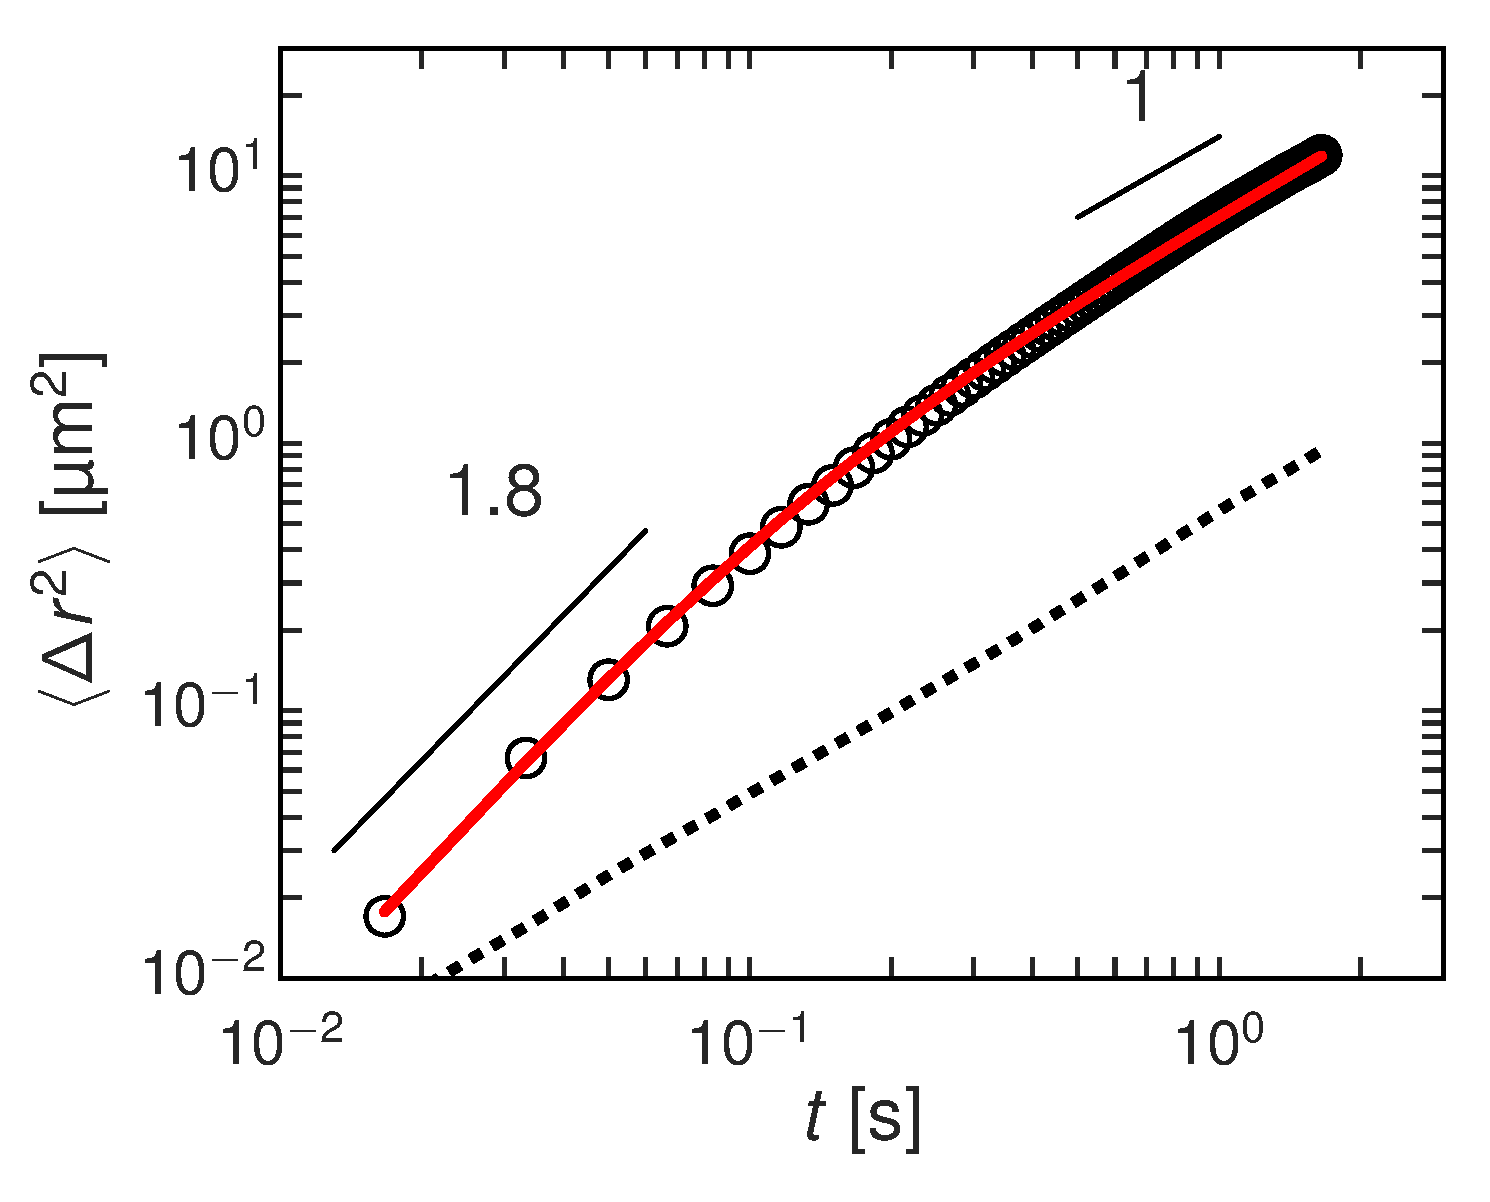
\includegraphics[width=\columnwidth]{bacteria/R1-active-msd}
  \caption{Ensemble-average mean-squared displacement of colloidal tracers during the initial, active stage of biofilm formation at an oil-water interface.  For reference, the dashed line displays the mean-squared displacement of colloids at the oil-water interface in the absence of bacteria.  The solid line displays the result of a fit using Eq. \ref{eqn:mss-memory}.}
  \label{fig:R1}
\end{figure}

Figure \ref{fig:R1} shows the colloids� ensemble-average mean-squared displacement, $\langle \Delta r^2 (t)\rangle = \langle(\vec{r}_i (t' + t) - \vec{r}(t')\rangle_{i, t'}$where the average is over particles i and time t�, during this active stage of biofilm formation.  For reference, the mean-squared displacement of colloids at the oil interface of pure Instant Ocean containing no bacteria is also shown.  In the absence of bacteria, $\langle \Delta r^2 (t) \rangle$ varies linearly with lag time t indicating simple diffusion, $\langle \Delta r^2 (t) \rangle=4D_0 t$, with a diffusion coefficient, $D_0 = 0.12 \mu m^2/s$, consistent with the viscosities of water and hexadecane.  The mean-squared displacement of the colloids at the active interface similarly varies linearly with t at large lag times, but with an enhanced effective diffusion coefficient.  At smaller lag times, the mean-squared displacement grows more rapidly than linearly, indicating superdiffusive motion.  Such superdiffusive motion is a common feature of colloidal motion in microbial suspensions and signals temporal correlations in the forcing of the colloids due to hydrodynamic interactions with the swimmers.  A simple model for these correlations ascribes to them a single characteristic correlation time ?, so that the particle velocities have an exponentially decaying memory, $\vec{v}(t')\cdot\vec{v}(t' + t)\sim \exp(-t/\tau)$[WuPRL2000].  Such velocity correlations lead directly to a mean-squared displacement of the form [KurtulduPNAS2011]

\begin{equation}
\langle \Delta r^2 (t) \rangle = 4D\left[t + \tau(e^{-t/\tau} - 1)\right]
\label{eqn:mss-memory}
\end{equation}

\noindent In the limit of short lag times, t << ?, this form predicts ballistic motion, $\langle \Delta r^2 (t) \rangle=\frac{2D}{\tau}t^2$; and at large lag times it reduces to diffusive motion, $\langle \Delta r^2 (t) \rangle=4Dt$, with effective diffusion coefficient $D$.   The solid line in Fig.\ref{fig:R1} is the result of a fit using this form, which describes data accurately and gives $D =1.8�0.1 \mu m^2/s$ and $\tau = 0.053 \pm 0.007$ s.   The value of $D$ in relation to the diffusivity in the absence of bacteria, $D/D_0\approx15$, indicates that biomixing strongly influences the interface during this early stage of biofilm formation.  We note further that this factor likely underestimates the enhancement in tracer mobility due to the swimming bacteria since, as described below, even at these early interface ages the incipient biofilm imparts an interfacial viscosity that reduces thermal diffusivity.

The success of Eq. (\ref{msd-memeory}) in capturing the form of $\langle \Delta r^2 (t) \rangle$ is consistent with several earlier studies of colloidal motion in active microbial suspensions and hence indicates that the velocities of tracers in such suspensions indeed have exponentially decaying memory.  However, we can interrogate these correlations more directly by defining an instantaneous direction of motion for each particle,

\begin{equation}
\hat{n}(t) = \frac{\vec{r}_i(t) - \vec{r}_i(t + \delta t)}{|\vec{r}_i(t) - \vec{r}_i(t + \delta t)|}
\end{equation}

\noindent where $\delta t = 1/60$ s is the time between successive video frames and $i$ labels the particles, and by examining its time-time autocorrelation function,

\begin{equation}
\Phi_n(t) = \langle\hat{n}_i(t + t')\cdot\hat{n}_i(t)\rangle_{i,t'}
\end{equation}

\begin{figure}[htbp]
  \centering
  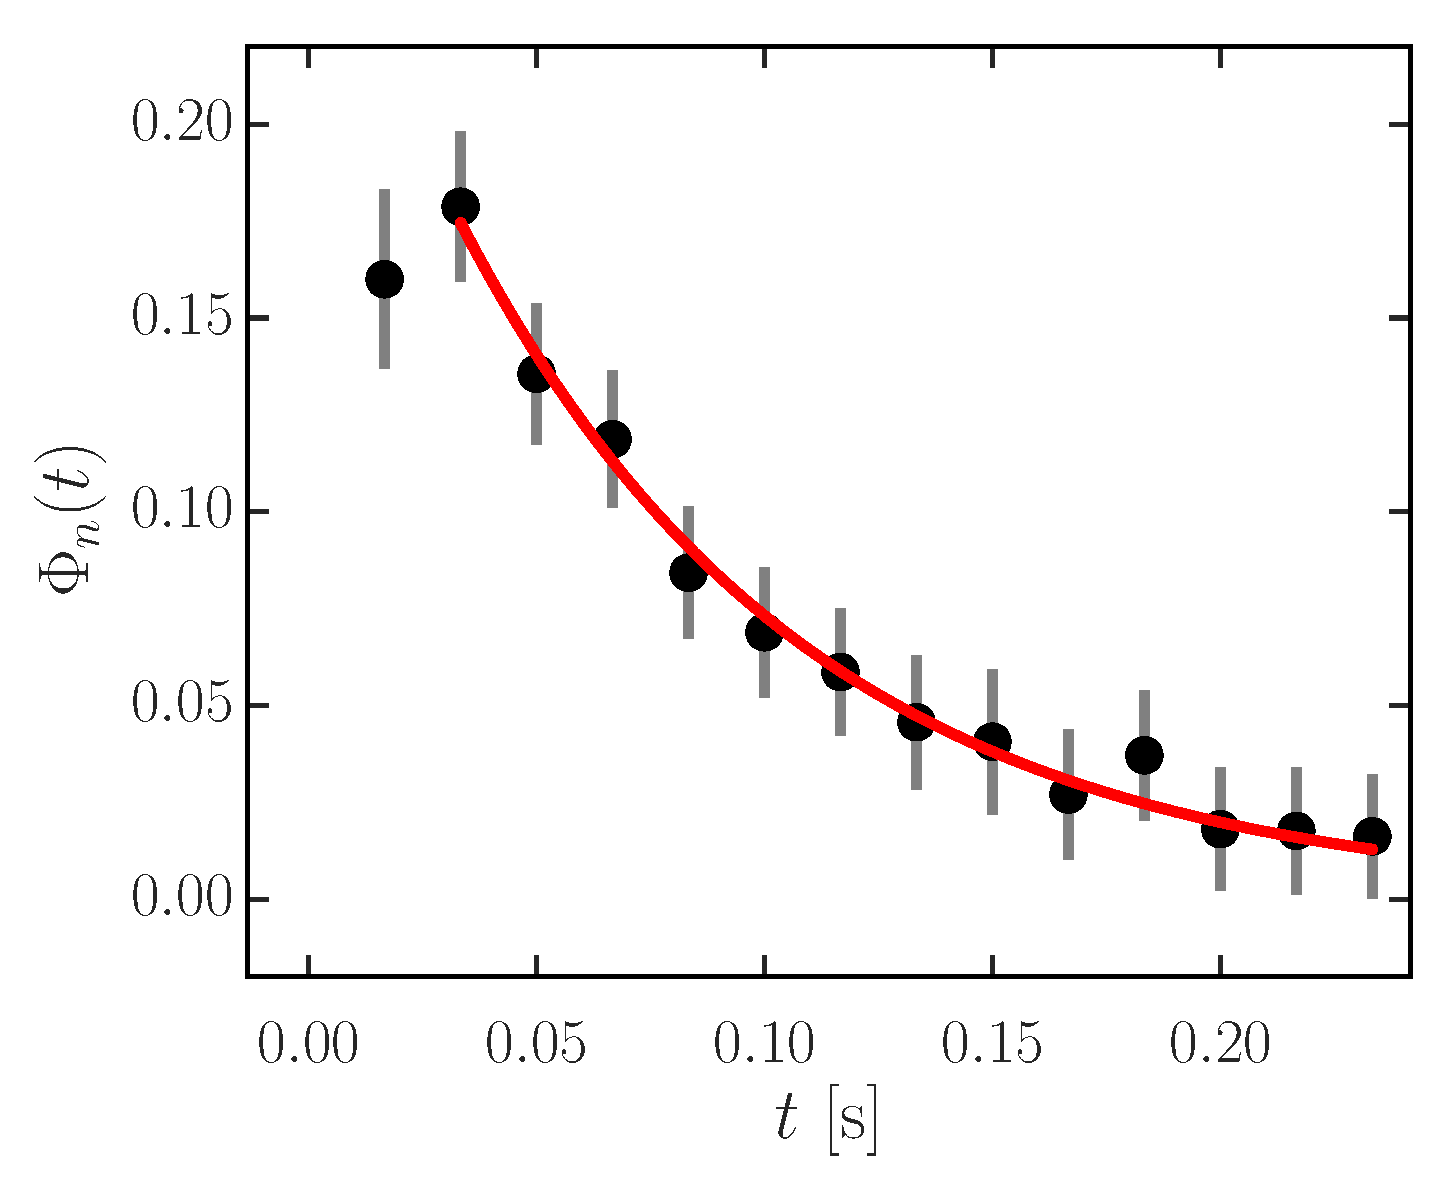
\includegraphics[width=\columnwidth]{bacteria/R2-time-autocorrelation}
  \caption{Time autocorrelation function of the direction of instantaneous tracer displacements during the active stage of biofilm formation.  The line shows the result of an exponential fit to the data at large times ($t > 0.03$ s).}
  \label{fig:R2}
\end{figure}

The significance of $\Phi_n (t)$ is that it quantifies the persistence in the direction of the colloids� trajectories.  As shown in Fig. \ref{fig:R2}, $\Phi_n (t)$ is effectively zero at $t > 0.15$ s, setting the typical time required for the colloids� direction of motion to randomize completely.  Notably, $\Phi_n (t)$ does not decay monotonically but has a peak near $t = 0.03 $s.  We attribute this peak to a tendency for colloids to follow ``U-shaped'' trajectories on short time scales due to hydrodynamic interactions with bacteria swimming past in close proximity [Leptos], and hence to make negative contributions to $\Phi_n (t)$.  At larger times, $\Phi_n (t)$ decays exponentially, as shown by the line in Fig. \ref{fig:R2}, which is an exponential fit to the data.  The correlation time obtained from the fit is $0.075 \pm 0.01$ s, which is in reasonable agreement with the characteristic time $\tau$ for velocity correlations implied by fitting $\langle \Delta r^2 (t)\rangle$ with Eq. (\ref{msd-memory}).  Thus, through $\Phi_n (t)$ we observe directly the nature of the correlated tracer dynamics in an active suspension inferred by the analysis of $\langle \Delta r^2 (t)\rangle$.

\begin{figure}[htbp]
  \centering
  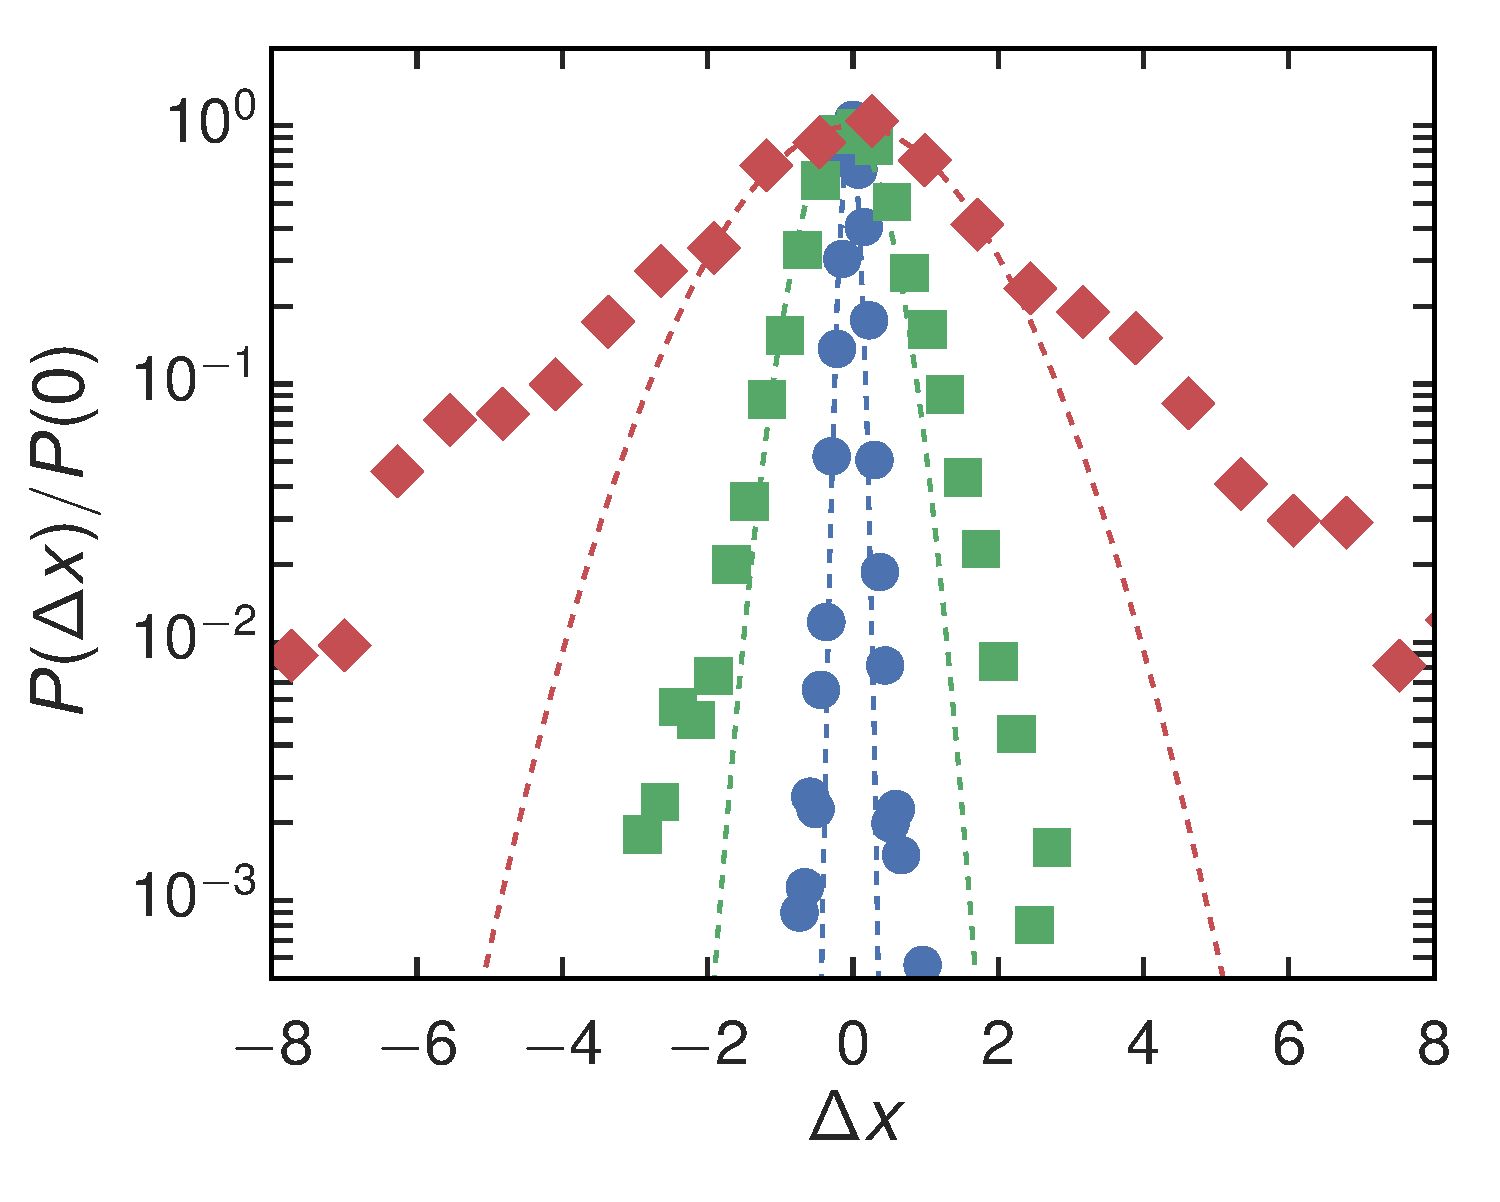
\includegraphics[width=\columnwidth]{bacteria/R3-Active-nongaussian-van-Hove}
  \caption{Normalized probability distribution functions for colloidal displacements at lag times of 0.016 s (blue), 0.15 s (green), and 1.3 s (red) during the active stage of biofilm formation.  The solid lines display the results of fitting Gaussian lineshapes in the regions of the peaks of the distributions, highlighting the enhanced, non-Gaussian probability for large displacements.}
  \label{fig:R3}
\end{figure}


While the colloids� Brownian dynamics at large lag times with diffusivity $D$ suggest that the suspension of swimming bacteria act like a thermal bath with large effective temperature, several previous studies have emphasized that the statistical properties of the colloidal displacements differ from those expected for a system in thermal equilibrium [ChenPRL2007, LeptosPRL2009, KurtulduPNAS2011].  These differences are apparent in the probability distribution function (PDF) for displacements at fixed lag time $P_t (\Delta x)$, where $\Delta x$ is the displacement along one direction.  Figure \ref{fig:R3} shows $P_t (\Delta x)$ at $t = 0.0167$ s, 0.15 s, and 1.3 s, lag times spanning the superdiffusive and diffusive behavior in $\langle \Delta r^2 (t)\rangle$.  The PDFs of particles undergoing thermal diffusion in equilibrium would be Gaussian.  In all cases, the PDFs in the active, incipient biofilm show clear deviations from Gaussian forms, with tails at large $|\Delta x|$ that signal enhanced probability of large displacements.  Qualitatively similar non-Gaussian PDFs have been observed previously among tracers in microbial suspensions and have been associated with advection-enhanced large displacements due to hydrodynamic encounters between the colloids and swimmers [LeptosPRL2009, KurtulduPNAS2011].  To compare the form and magnitude of the non-Gaussian contributions to $P_t (\Delta x)$ at different lag times more closely, we plot in Fig. \ref{fig:R4} the normalized PDFs with displacement normalized by the root mean-squared displacement.  Remarkably, the normalized PDFs collapse onto a single lineshape, indicating that the distribution function maintains a self-similar form with increasing lag time.  Such self similarity is generally unexpected and implies particular attributes about the colloidal dynamics, including (i) that the fraction of colloids in the non-Gaussian population remains constant over the range of lag times probed, and (ii) that the Gaussian and non-Gaussian displacements grow as the same function of lag time, first superdiffusively at short lag times and then diffusively at longer lag times.  Self-similar distributions with non-Gaussian tails were also observed among tracer displacements within bulk (3D) suspensions of the eukaryotic microorganism Chlamydomonas [LeptosPRL2009].  However, in that case, $\langle \Delta r^2 (t)\rangle$ displayed diffusive behavior over the entire range of lag times probed.  The collapse in Fig. \ref{fig:R4} is particularly notable because the lag times span both the superdiffusive and diffusive regimes.  In both the previous case of tracers among swimming Chlamydomonas and in our case of tracers in an incipient biofilm, the non-Gaussian contributions to the probability distribution function follow a Laplace distribution, so that the total PDF can described as the sum of two parts,

\begin{equation}
\label{eq:gaussian-laplacian}
P(\Delta x) = \frac{1 - f}{\sqrt{2\pi\sigma^2}}\exp\left[-\frac{1}{2}\frac{\Delta x}{\sigma}^2\right] + \frac{f}{\xi}\exp\left[-\frac{|\Delta x|}{\xi}\right]
\end{equation}

\noindent The solid line in Fig. \ref{fig:R4} is the result of a fit to the data using this form.

\begin{figure}[htbp]
  \centering
  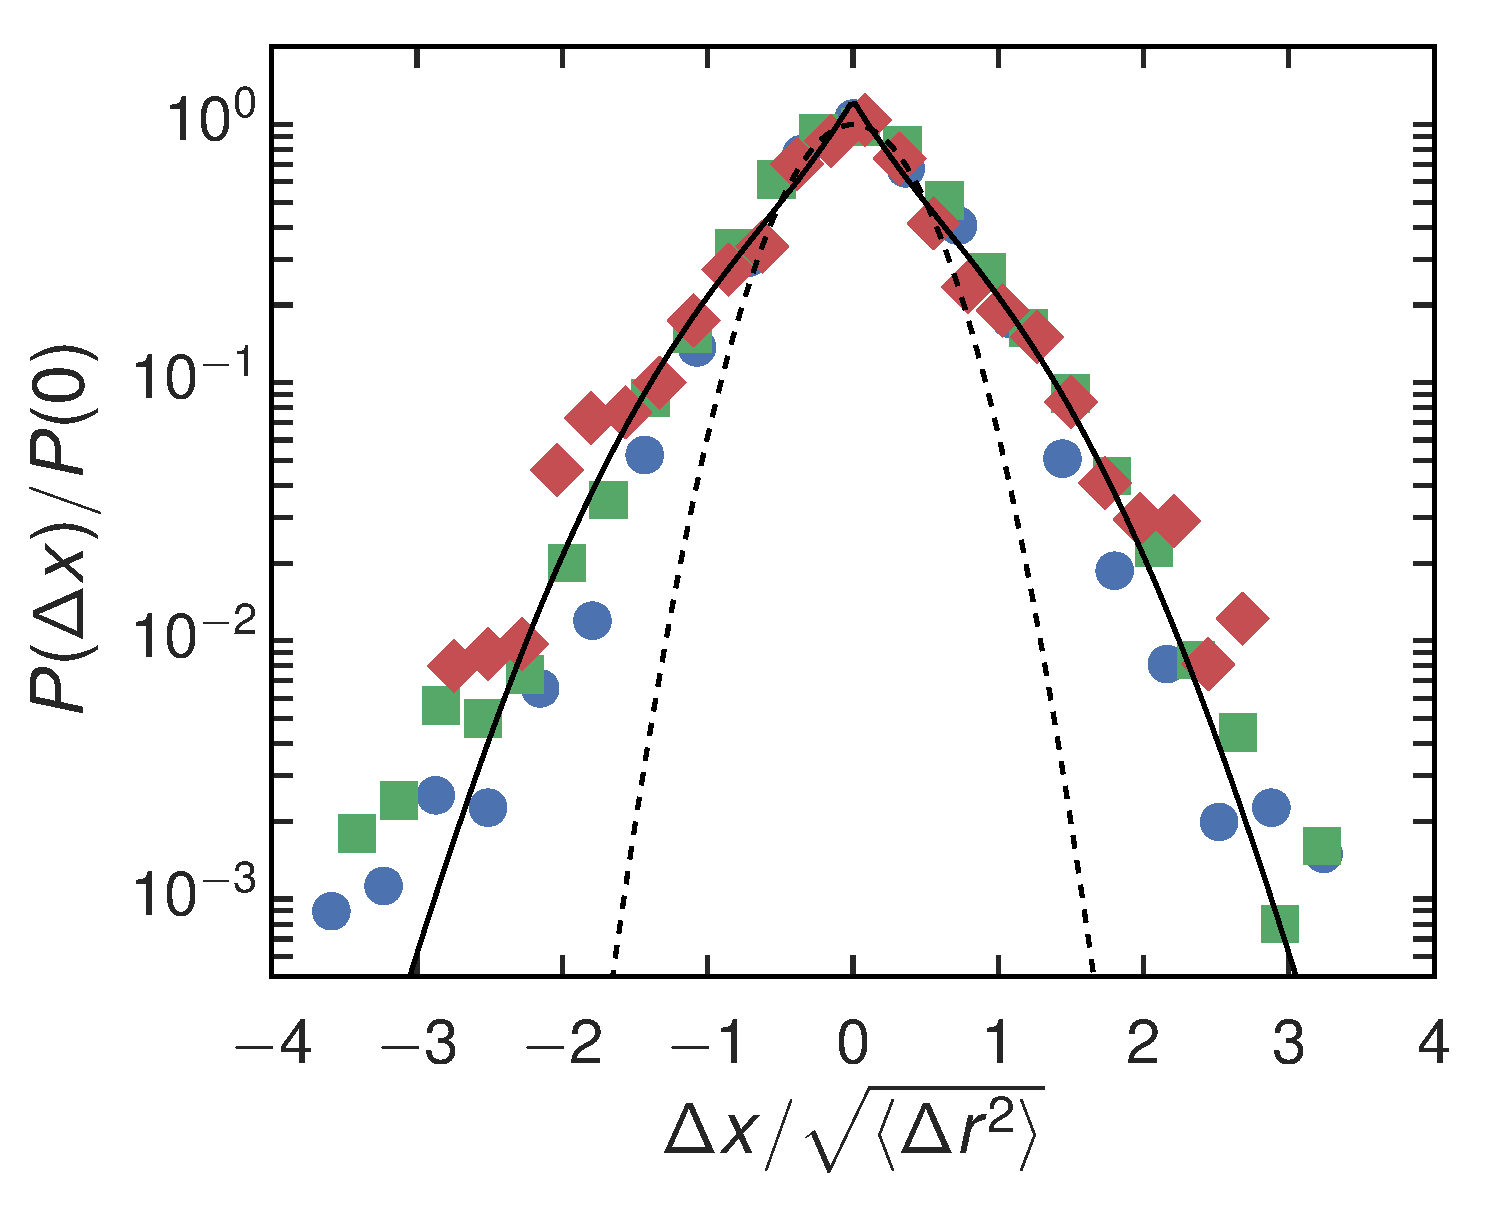
\includegraphics[width=\columnwidth]{bacteria/R4-Active-nongaussian-van-Hove-rescaled}
  \caption{Normalized probability distribution functions from Figure \ref{fig:R3} plotted against displacement normalized by the root mean squared displacement at each lag time, illustrating the collapse of the distributions onto a common lineshape.  The dashed line displays the result of fitting a Gaussian lineshape in the regions of the peak.  The solid line displays the result of a fit using the form given by Eq. \ref{eqn:gaussian-laplacian}}
  \label{fig:R4}
\end{figure}

The strong similarity between the self-similar PDFs of tracer displacements in the incipient interfacial bacterial biofilm and those in bulk suspensions of Chlamydomonas is surprising since the tracer displacements in quasi-2D films of the Chlamydomonas suspensions display qualitatively different non-Gaussian distributions, and the authors of those studies attributed the difference to the differing fluid velocity fields generated by the force dipoles of the Chlamydomonas swimming in two and three dimensions [KurtulduPNAS2011].   Our case of colloids entrained at an oil interface of a suspension of swimming bacteria that are forming a biofilm has several features that distinguish it from these studies.  First, the colloids, while in the incipient biofilm, were in contact with the aqueous subphase and hence were coupled hydrodynamically to bacteria both in the film and in the bulk, a situation that is in some sense a hybrid of the three-dimensional and quasi-two-dimensional systems considered previously.  Second, as discussed below, biofilm formation substantially impacts the rheology of the interface even at the earliest ages, with possible qualitative consequences on the coupling between the swimming bacteria and the colloidal tracers in the film.  Finally, Chlamydomonas is a ``puller'' while Pseudomonas sp. is a ``pusher,'' and this distinction has consequences for the collective behavior and resulting hydrodynamics of suspensions.  Given these distinctions, the strong correspondence between the PDFs in Fig. \ref{fig:R4} and those from bulk Chlamydomonas suspensions suggests that such self-similar distributions with Gaussian and Laplacian components might emerge more generically in nonequilibrium active systems than previous thought.

\begin{figure}[htbp]
  \centering
  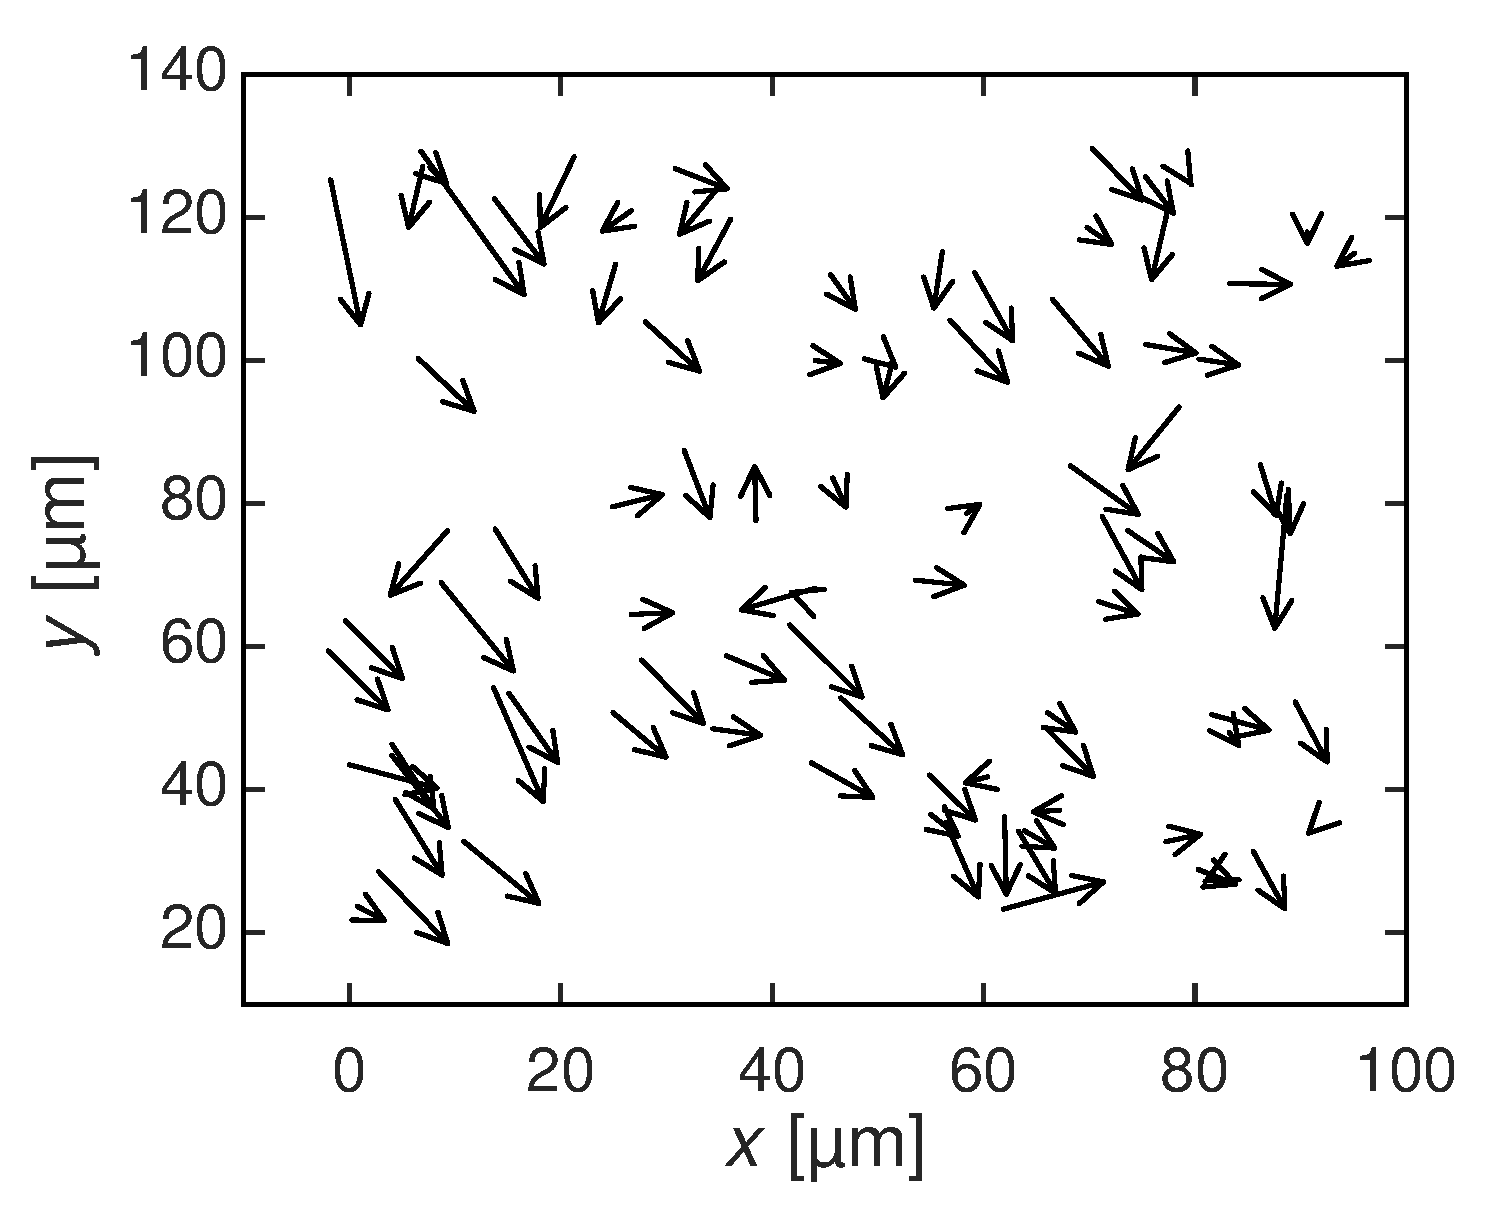
\includegraphics[width=\columnwidth]{bacteria/R5-displacement-arrows}
  \caption{Map of a section of the interface during the active stage of biofilm formation showing the direction of motion of the colloidal tracers at an instant in time. Each colloid is represented by an arrowhead indicating its instantaneous motion $\vec{r}$.}
  \label{fig:R5}
\end{figure}

Another feature of our study of the active stage was the density of colloidal probes at the interface, which was large enough that correlated motion among the colloids could be observed, thereby providing information about the spatial correlations of the non-Brownian �kicks� the swimming bacteria impose.  As an illustration, Figure \ref{fig:R5} depicts $\vec{r}$ for the colloids in the microscope field of view at one instant during the active stage.  Alignment between the direction of motion of nearby colloids is clearly apparent.  This coordinated motion is quantified in Fig. \ref{fig:R6}, which shows the normalized pair direction-direction correlation function,

\begin{equation}
C_n(r) = \langle \hat{n}_i\cdot\hat{n}_j\rangle_{i,j,t}
\end{equation}

where the brackets represent an average over all pairs of particles $i, j$ separated by distance $r$. The spatial correlations in tracer motion decay exponentially with separation, as depicted by the dashed line in Fig. \ref{fig:R6}, which is the result of an exponential fit to the data with correlation length of  $4.7 \pm 1.7 ?m$.  Together, $G_n (t)$ and $C_n (r)$ give a quantitative picture of the short-time, spatiotemporal correlations in tracer motion that characterize the dynamical behavior of the interface during the initial, active stage of biofilm development. 

\begin{figure}[htbp]
  \centering
  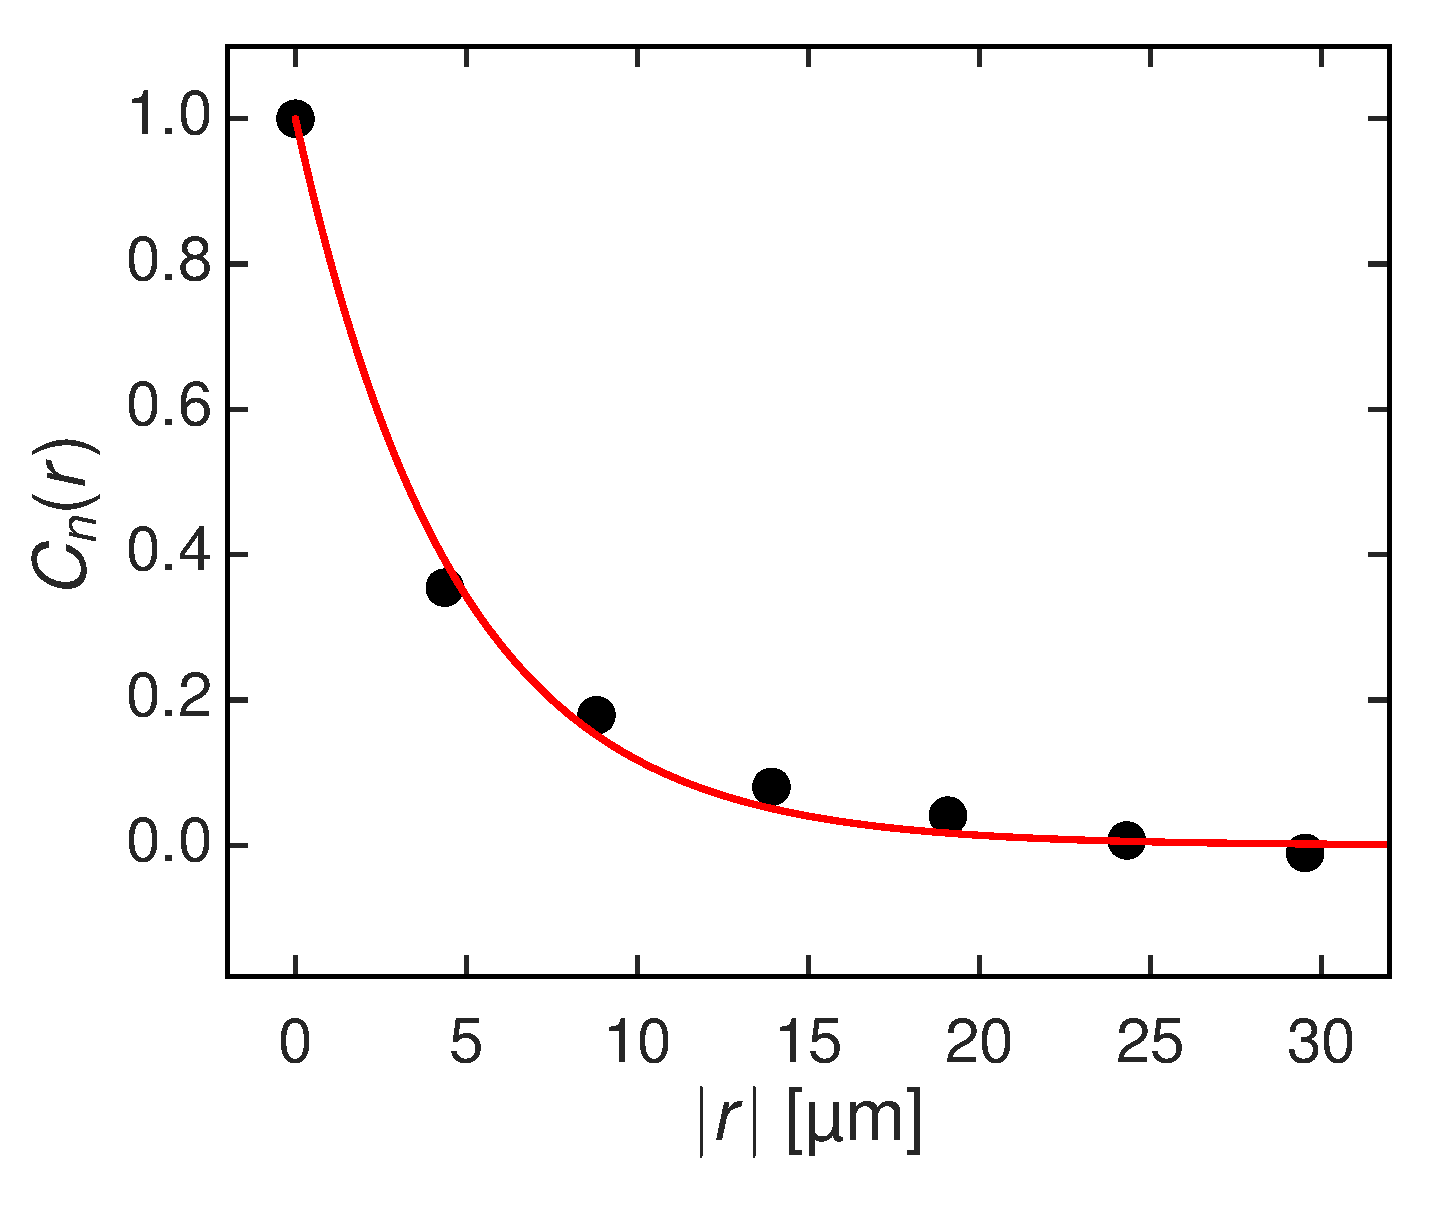
\includegraphics[width=\columnwidth]{bacteria/R6-Cn}
  \caption{Normalized pair direction-direction correlation function as a function of the distance between colloids during the active stage of biofilm development.}
  \label{fig:R6}
\end{figure}

\subsection{Viscoelastic Transition}

Typically, the initial active stage of the biofilm persisted for less than 5 minutes, after which no motile bacteria were observed either at the surface or in the near-surface bulk.  We ascribe the limited duration of the bacteria motility to the lack of nutrient in the suspension.  The end to the active stage was reflected in a qualitative change to the probe dynamics in which the probe mean-squared displacement changed from superdiffusive at short lag times to subdiffusive.  Once the bacteria ceased to move visibly, we treated the interface as a passive system close to thermodynamic equilibrium and considered the probes to be undergoing thermally-driven Brownian trajectories from which the film rheology could be inferred.
 As mentioned above, the active stage was not always observed.  Significantly, the ensuing mechanical changes of the interface, as inferred from probe mobility, appeared qualitatively independent of whether it was preceded by an active stage. Furthermore, as discussed below, the evolution in film rheology persisted for many minutes after the end of the active stage, suggesting that the presence of absence of an active stage had limited impact on subsequent biofilm evolution.  From these observations we conclude that the film formation was primarily the consequence of polysaccharides and surface-active moieties produced by the non-motile (resting?) bacteria.  However, we cannot discount the possibility of some subtle effects to biofilm formation due to biomixing by the swimming bacteria in those instances with an active stage.
Here, we present results for the viscoelastic evolution of the biofilm from an experiment in which no protracted active stage was visible at the start of film formation.  We focus on this data set because (i) the population of (non-motile) bacteria at the interface was limited, leaving a relatively unobstructed interface for the colloids and facilitating the analysis of their Brownian motion, and (ii) the colloidal motion was less likely to be affected by any residual activity than in a trial with a fully realized active stage.  We emphasize again that the trends observed were qualitatively the same as those in trials in which the viscoelastic film development was preceded by an active stage.

\begin{figure}[htbp]
  \centering
  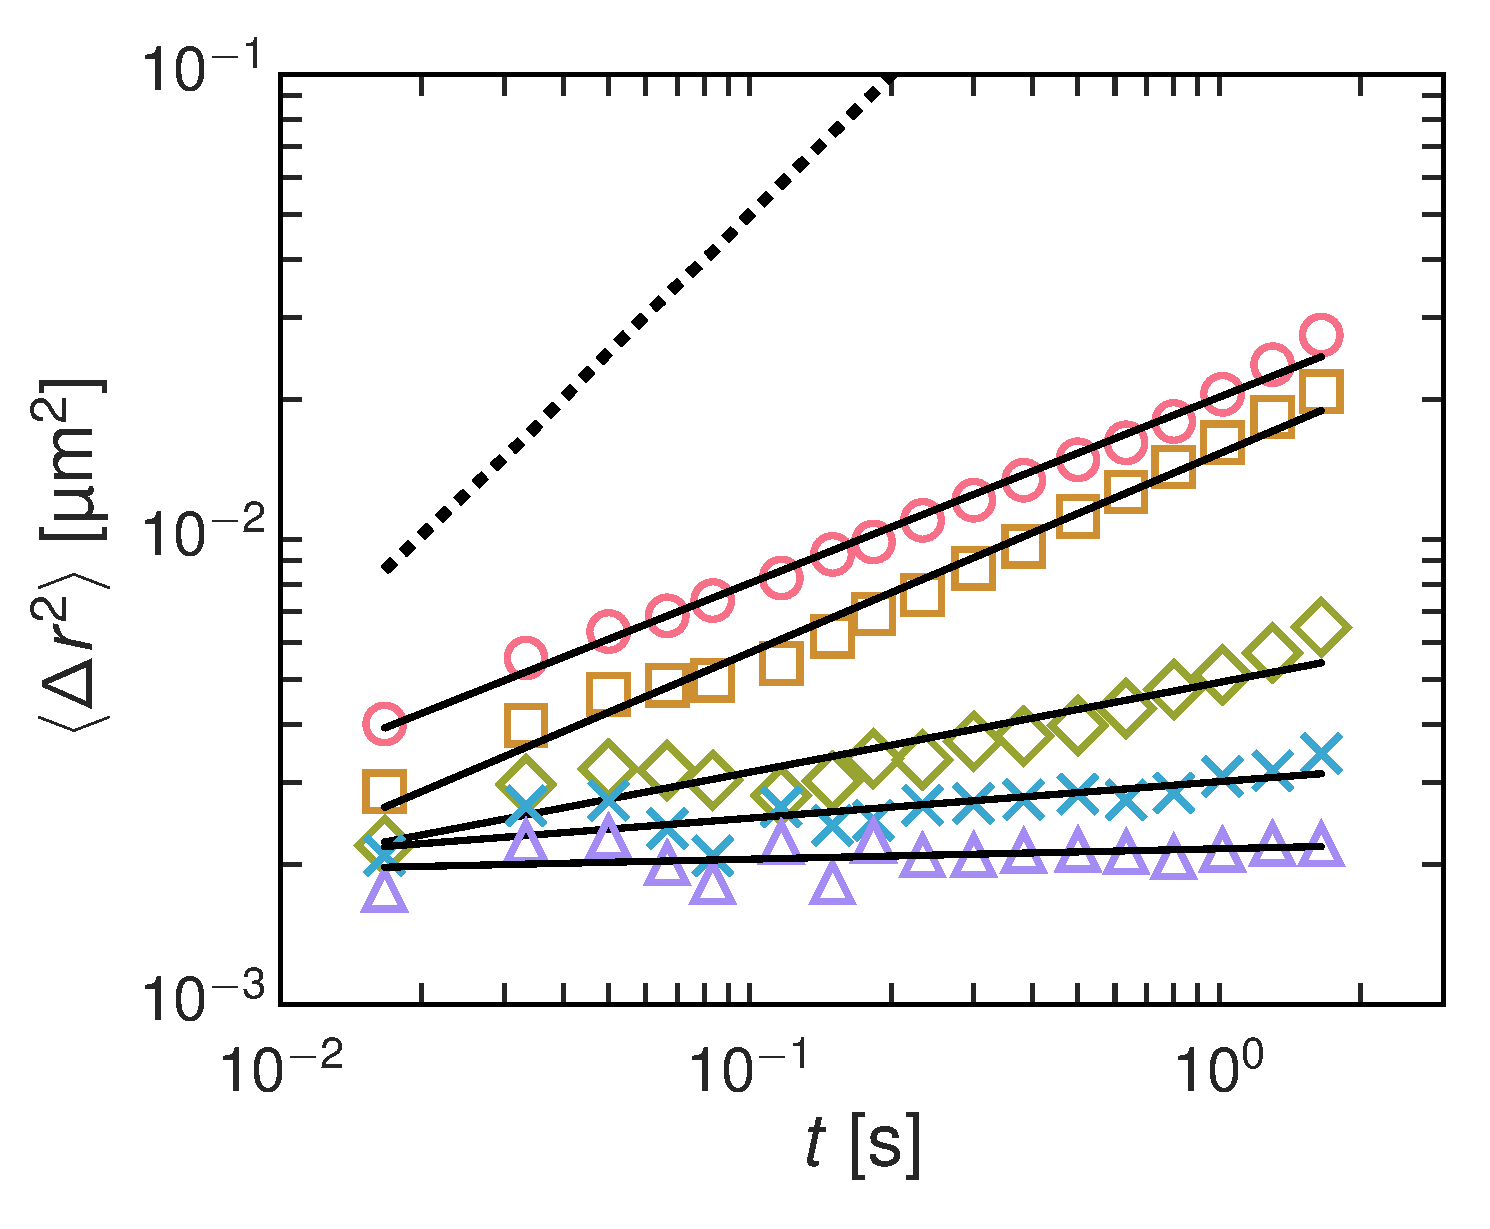
\includegraphics[width=\columnwidth]{bacteria/R7-transition-ensemble-msds}
  \caption{Ensemble-average mean squared displacement of colloids at several ages (red circles: 57 seconds, orange squares: 360, green diamonds: 1080, blue X�s: 10080, purple triangles: 88920) during biofilm formation at an oil-water interface for a trial with no active stage.  For reference, the dashed line displays the mean squared displacement of colloids at the bare oil-water interface in the absence of bacteria.  The solid lines display the result of power-law fits.}
  \label{fig:R7}
\end{figure}

Figure \ref{fig:R7} shows the ensemble-averaged mean-squared displacement $\langle \Delta r^2 (t)\rangle$ of the colloidal probes at several ages ta of biofilm formation following creation of the interface.  Because each mean-squared displacement is determined from 1 minute of video, the maximum lag time t is restricted to $t < 2$ s to assure adequate statistics.  Again for reference, the mean-squared displacement of colloids diffusing at the oil interface of pure Instant Ocean containing no bacteria is also shown.  At our earliest measurement of biofilm formation, the colloidal mean-squared displacement varies sublinearly with lag time, indicating a drag due to the development of a film with viscoelastic character. 
Within the limited dynamic range of accessible lag times, $\langle \Delta r^2 (t)\rangle$ is approximated as a power law, $\langle \Delta r^2 (t)\rangle \sim t^n$, with $n < 1$. As shown in Fig. \ref{fig:R8}, the power-law exponent $n$ decreases steadily with increasing age, signifying increasingly subdiffusive motion. While in principle the probe mobility is affected by both the interfacial film and drag from the surrounding bulk oil and water, given the large difference between $\langle \Delta r^2 (t)\rangle$ in the presence of the forming film and at the neat interface, we can safely infer that the bulk contributions to the drag are insignificant. In this case, under appropriate conditions one can obtain the frequency-dependent interfacial shear modulus, $G^*(\omega) = G'(\omega) + iG''(\omega)$, from the Brownian motion of the probes through a two-dimensional version of a generalized Stokes-Einstein relation, (Helfer2001, Maestro2011)

\begin{equation}
\label{eqn:gse}
G^*(\omega)=\frac{k_B T}{\pi i\omega\mathcal{F}_u\left\{\langle \Delta r^2 (t)\rangle\right\}}
\end{equation}

\noindent where $\mathcal{F}_u\left\{\langle \Delta r^2 (t)\rangle\right\}$ is the unilateral Fourier transform of the mean-squared displacement.  Following Eq. (\ref{eqn:gee}, power-law behavior in the mean-squared displacements of the colloidal probes, $\langle \Delta r^2 (t)\rangle \sim t^n$ with $n < 1$, implies the film�s shear modulus has power-law frequency dependence, $G'(\omega) \sim G''(\omega) ~ \omega n$  (Mason2000). 

\begin{figure}[htbp]
  \centering
  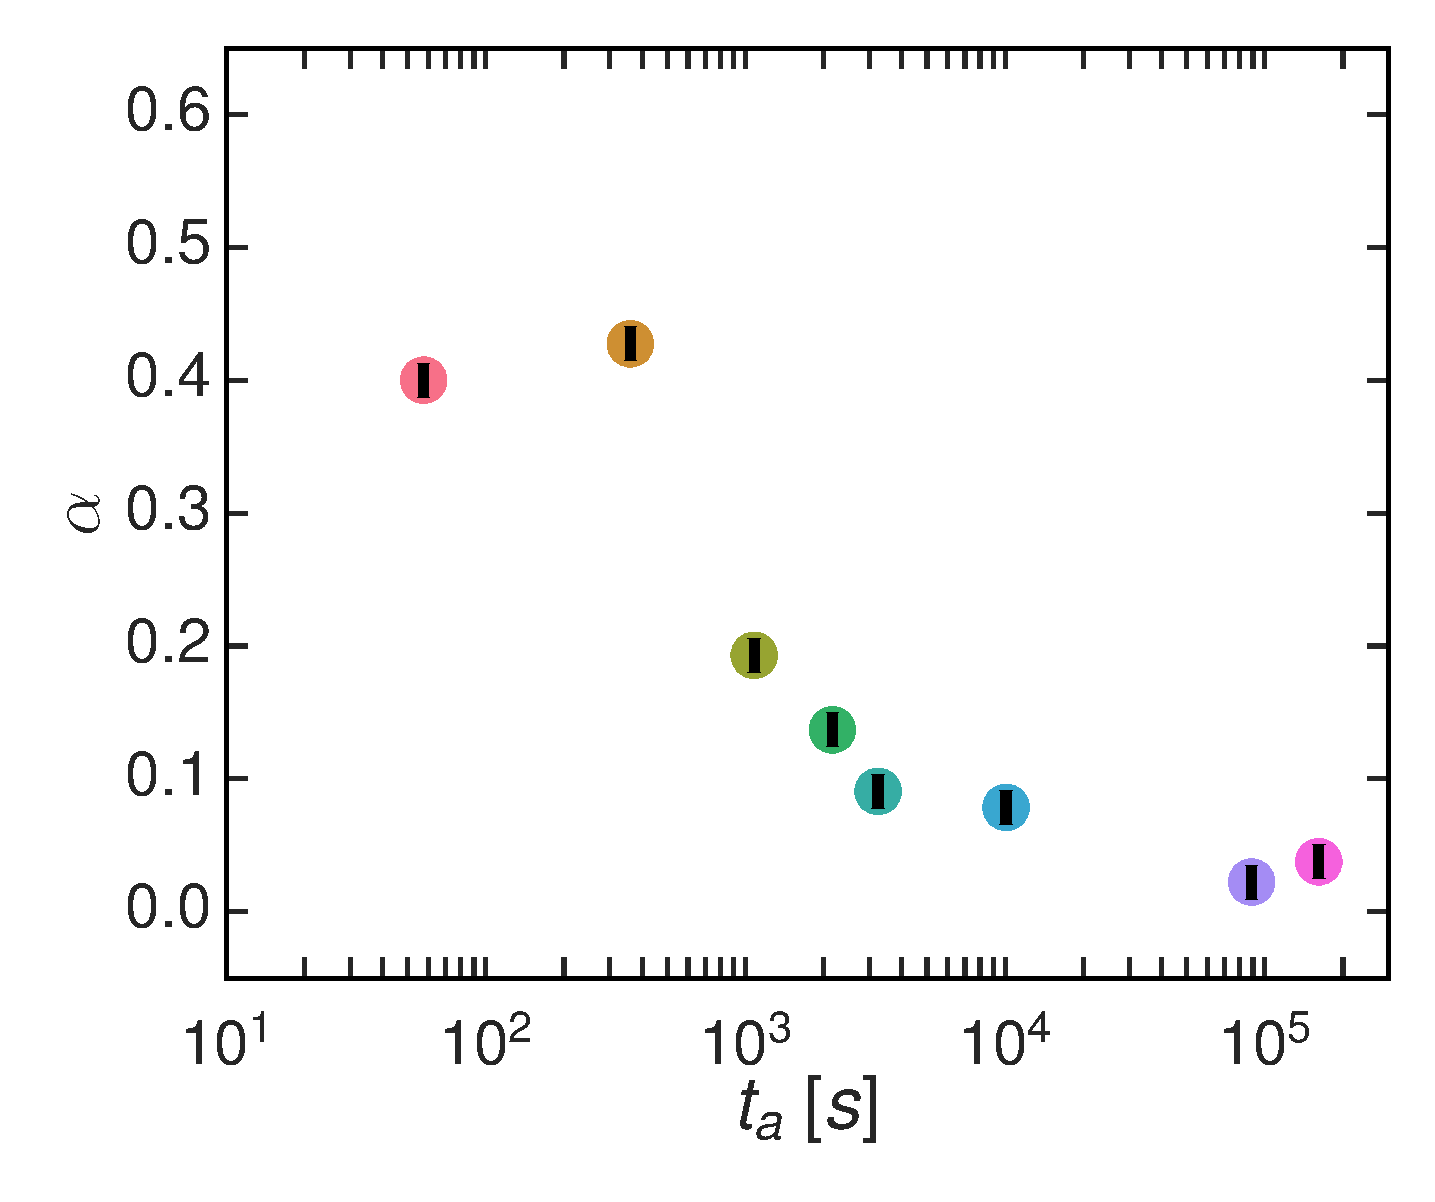
\includegraphics[width=\columnwidth]{bacteria/R8-transition-power-law-exp}
  \caption{Power-law exponent characterizing the ensemble average mean-squared displacements, $\langle \Delta r^2 (t)\rangle \sim t^{\alpha}$, of colloids the oil-bacteria solution interface as a function of the age since formation of the interface.}
  \label{fig:R8}
\end{figure}

\begin{figure}[htbp]
  \centerline{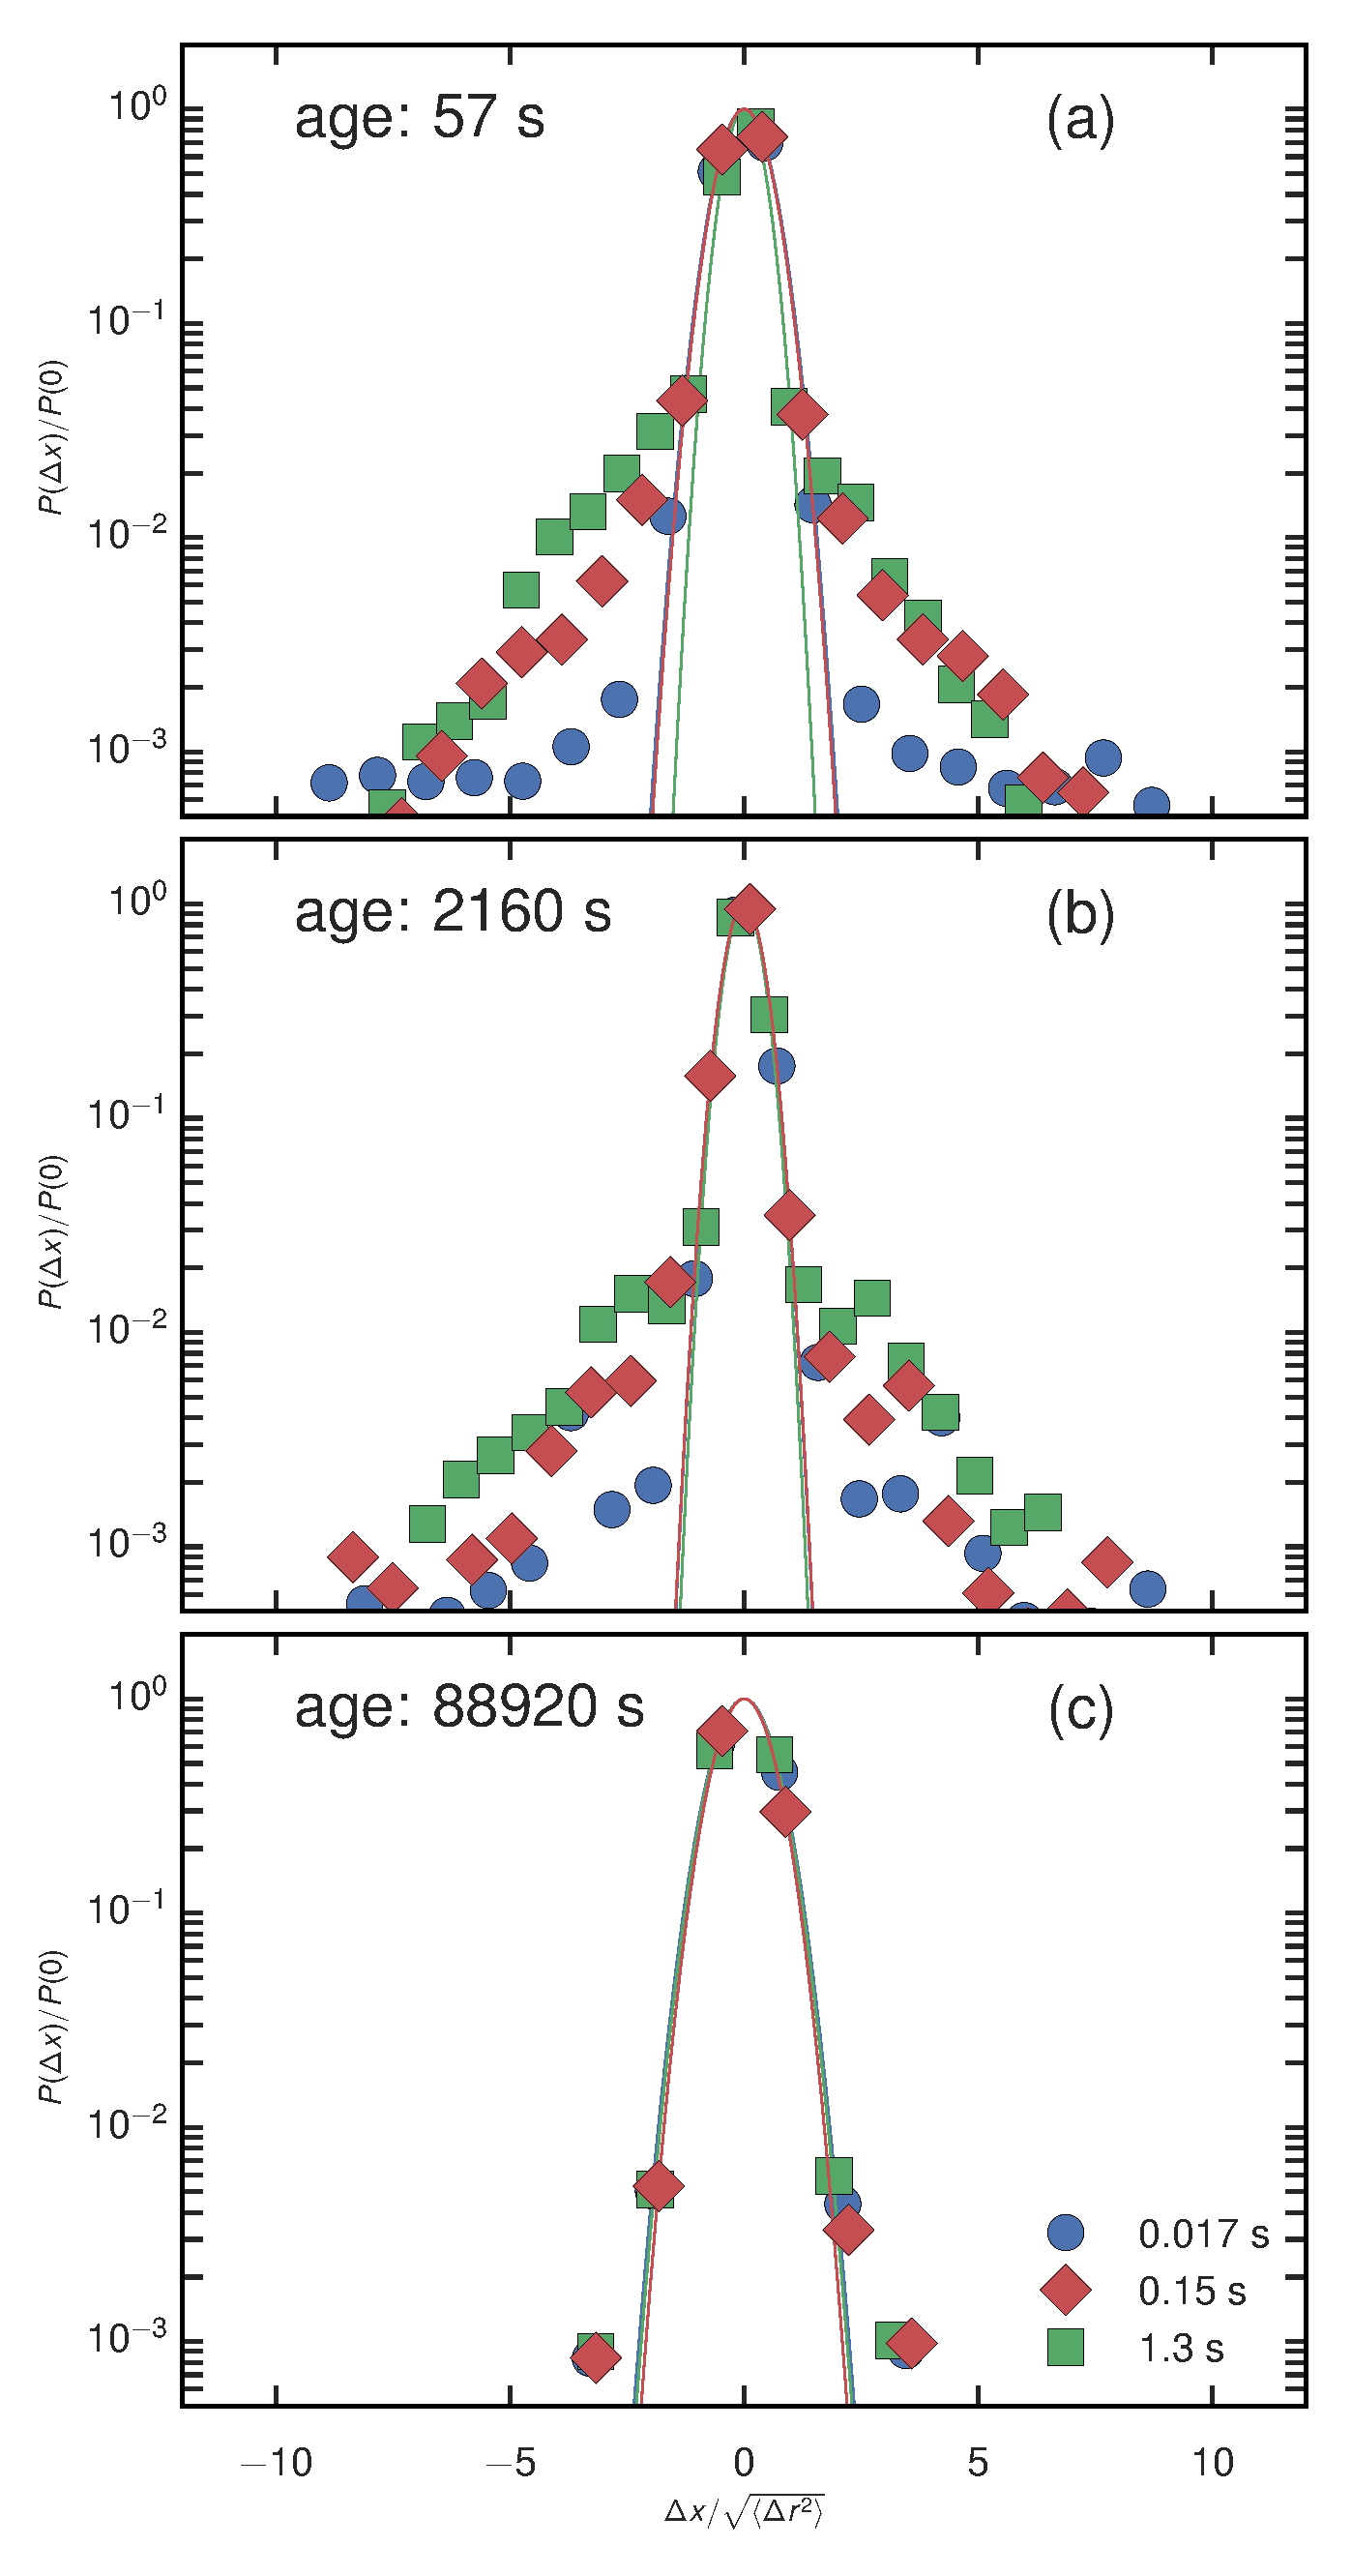
\includegraphics[width=\columnwidth,height=0.8\textheight,keepaspectratio]{bacteria/R9-viscoelastic-transition-vanhove-collapse}}
  \caption{Normalized probability distribution functions for colloidal displacements at lag times of 0.016 s (blue), 0.15 s (green), and 1.3 s (red) at film ages (a) 57 s, (b) 2160 s, and (c) 88920 s during the viscoelastic stage of biofilm formation.  The solid lines display the results of fitting Gaussian lineshapes in the regions of the peaks of the distributions, highlighting the enhanced, non-Gaussian probability for large displacements.}
  \label{fig:R9}
\end{figure}

Such weak power-law frequency dependence of $G^*(\omega)$ is characteristic of the rheology of a broad range of disordered complex fluids including concentrated microgel solutions (Ketz1988), foams, (Khan1988) paint, (Mackley1994) intracellular matrix,(Fabry2001) compressed emulsions, (Mason1995)  clay suspensions, (Bonn2002) and liquid-crystal nanocomposites (Bandyopadhyay2005) and is indicative of a broad spectrum of relaxation times.  In most cases, the power-law exponent typically lies in the range $n\approx$ 0.1 to 0.3.  The soft glassy rheology model (Sollich1998) explains this response as a general consequence of structural disorder and metastability, and provides a unifying theoretical framework for this behavior.  In this model, $n$ serves as an effective noise temperature, with systems approaching a glass transition as $n\rightarrow 0$.  Thus, the steady decrease in $n$ with layer age reported in Fig. \ref{fig:R8} points to increasingly glassy dynamics characterizing the structural response of the biofilm.  
An important property of soft glassy systems is their non-equilibrium behavior and spatial heterogeneity.  As a measure of these features, Figs. \ref{fig:R9}(a)-(c) show the PDFs of colloidal displacements at three ages during the viscoelastic transition.  In each case, the PDF is shown at three lag times normalized by the mean-squared displacement at that lag time.  At the earlier two ages, ($t_a$ = ??? and ???), during which the viscoelastic character of the film is evolving rapidly, the PDFs show a pronounced non-Gaussian components corresponding to enhanced probability of large displacements.  These non-Gaussian contributions resemble those characterizing the colloidal dynamics in the active stage (Figs. \ref{fig:R3} and \ref{fig:R4}); however, their origin in this case is different.  Unlike at the active interface, the perturbations here are thermal, and each individual particle�s displacements are Gaussian.  The non-Gaussian distributions result from variation in the mobility of different particles, evincing a spatially heterogeneous interface of rheological microenvironments [Valentine 2001].  Surprisingly, this heterogeneity diminishes at late ages, as illustrated by the closer-to-Gaussian distributions in Fig. \ref{fig:R9}(c), when the interface�s evolution has slowed and the film is nearly elastic.  An interesting future study would be to compare this spatial heterogeneity with that of films formed in the presence of an extended stage of activity by swimming bacteria to investigate the role of biomixing in suppressing such heterogeneity. 
 
% !TEX root = root.tex
\chapter{\label{chap:photoactivation}Multiscale Nanoparticle Mobility Measurements in Biological Gels Using Photoactivatable Fluorescent Probes}
\chaptermark{Photoactivation}

\section{Introduction}

Drug-delivery nanoparticles often must diffuse through biological barriers to achieve therapeutic efficacy at their target site. In some instances, such as tear film at the ocular surface, the barrier is only a few micrometers thick \cite{King-Smith2000,Azartash2011}. In other cases, nanoparticles must penetrate tens of micrometers or more through viscoelastic biological gels or tissue \cite{Nance2012,Xu2013,Schuster2013}. Measurements \emph{in vitro} at physiologically relevant length scales are valuable for designing nanoparticles that will exhibit favorable \emph{in vivo} biodistribution.
Here, we present a strategy for measuring nanoparticle mobility in biological gels over length scales ranging from sub-micrometer to tens of micrometers using photoactivatable fluorescent probes. This work is part of a collaboration with Benjamin Schuster and Joshua Kays in the laboratory of Professor Justin Hanes in the Center for Nanomedicine of JHU.

The study involved polymeric nanoparticles with a dense polyethylene glycol (PEG) coating to minimize particle adhesion to the gel. The particle core was imbued with photoactivatable (caged) rhodamine, which becomes fluorescent only if the rhodamine is ``uncaged'' through momentary exposure to UV light. This functionality permitted us to selectively photoactivate a region of particles with a brief pulse of UV light, and then observe the spread of the fluorescent particles in the gel over tens of micrometers and tens of minutes, all using confocal microscopy. Complementing these measurements, we were also able to quantify the motion of the photoactivated particles at high spatiotemporal resolution --- tens of nanometers and tens of milliseconds --- using multiple particle tracking (MPT) on a widefield microscope. MPT has been harnessed recently to measure transport of drug delivery nanoparticles in many biological materials, including brain tissue\cite{Nance2012}, mucus\cite{Lai2009,Wang2008,Schuster2013}, vitreous\cite{Xu2013}, and inside cells\cite{Crocker2007}. MPT is a powerful technique that permits examination of individual particles and analysis of heterogeneous transport behavior. However, because of the limited depth-of-field of high-numerical-aperture objectives, tracking particles diffusing in three dimensions for more than a few seconds and a few micrometers is difficult. The photoactivation method described here provides another approach to directly observe percolation through biological gels over longer distance and time scales. Hence, particle tracking and the photoactivation technique are complementary methods that, together, permit multiscale diffusion measurements. 

We first confirmed agreement between measurements from MPT and the photoactivation technique on particles diffusing in water. Then, we applied our method to fibrin, a model protein gel system, and found that both MPT and the photoactivation method reveal mobile and immobile populations of particles. Finally, we examined nanoparticle diffusion in sputum collected from cystic fibrosis (CF) patients. Sputum is a major barrier to inhaled CF therapeutics, and our approach enabled us to measure particle diffusion over distances relevant to drug delivery in the lungs, revealing large-scale heterogeneity in the mobility that might be missed with techniques surveying motion over shorter length scales.
\section{Experimental Methods}
\subsection{Materials}
Cholalic acid sodium salt (CHA), NVOC2-5-carboxy-Q-rhodamine-NHS ester (caged rhodamine-NHS ester), N-hydroxysulfosuccinimide sodium salt (sulfo-NHS), and N-(3-Dimethylaminopropyl)-N'-ethylcarbodiimide hydrochloride (EDC) were purchased from Sigma-Aldrich (St. Louis, MO). Poly(lactide-co-glycolide(75:25)) amine endcap (PLGA-NH2), Mn 10kDa-15kDa was purchased from Polyscitech (West Lafayette, IN). Poly(lactide-co-glycolide(67:33))-polyethylene glycol (45kDa-5kDa) diblock copolymer (PLGA-PEG) was custom-synthesized by Jinan Daigang Biomaterial Co., Ltd, (Jinan, China). 5 kDa methoxy-PEG-amine was purchased from Creative PEGWorks (Winston Salem, NC). Fluorescent carboxylate-modified polystyrene microspheres (PS-COOH) of diameter 100, 200, and 500 nm were purchased from Molecular Probes (Eugene, Oregon). Human $\alpha$-thrombin (activity 3059 NIH U/ml) and human fibrinogen (plasminogen depleted, activity 100\%) were purchased from Enzyme Research Laboratories (South Bend, IN).
\subsection{Particles}
The particles were designed and synthesized by my collaborators, Benjamin Schuster and Joshua Kays. Their protocol is presented here for context.
\subsubsection{Labeling of PLGA with caged rhodamine}
Caged rhodamine-NHS ester and PLGA-amine were conjugated through formation of an amide bond. Briefly, 90 mg of PLGA-NH2 was added to 5 mg of caged rhodamine-NHS ester (for a slight molar excess of dye compared to PLGA, 1:1.23) and put under vacuum for 1 h. The mixture was then flushed with nitrogen gas, dissolved in 500 \textmu l of anhydrous dichloromethane (DCM), and reacted for 12 h at room temperature under nitrogen gas. Additional DCM was added as needed to facilitate transfer of the product into 10 ml of -20 $^\circ$C diethyl ether to precipitate the product. The PLGA, now conjugated with rhodamine, was washed twice in cold ether by centrifugation. Excess ether was decanted off and the final product, the purified PLGA, was placed in a lyophilizer (FreeZone 4.5 Plus; Labconco) for 12 h. The dried PLGA was stored at  -20 �C  in a shielded container to prevent exposure to incident UV light.
\subsubsection{Particle formulation: PS-PEG} 
PEGylated polystrene (PS-PEG) particles were used a control in particle tracking experiments to verify that the mobility photoactivatable particles was the same as more widely used PS-PEG particles. PS-PEG particles were prepared as previously described\cite{Nance2012} by coupling PS-COOH with PEG-amine using carbodiimide chemistry1. Generally, 100 \textmu l of stock (2\% solids) PS-COOH particle solution was added to borate buffer (pH 8) with 4 fold molar excess 5k mPEG-amine, EDC, and sulfo-NHS. The particles were reacted for at least 2 h, then washed three times by centrifugation and stored in DI water at 4� C.
\subsubsection{Particle formulation: PLGA-PEG}
Photoactivatable PLGA/PLGA-PEG nanoparticles were prepared by using the emulsion method according to the literature\cite{Xu2013}. Briefly, a 40 mg mixture (19:1 by mass) of PLGA-b-PEG5k and PLGA-caged rhodamine was dissolved in 400 \textmu l of DCM, making a 100 mg/ml solution. This solution was injected into an ice-cooled 5 ml of 0.5\% CHA aqueous solution, and sonicated at 30\% amplitude for 2 min using a 130 Watt probe sonicator (Sonics \& Materials, Newtown, CT) to form an oil-in-water emulsion of the organic phase (polymer and DCM) into the aqueous phase, stabilized by the CHA surfactant. The emulsion was immediately added to 35 ml of 0.5\% CHA solution and stirred at 600 rpm for at least 3 h to allow for complete particle hardening. The final particle suspension was filtered through a 5 \textmu m and then 0.45 \textmu m syringe filter, then the particles were collected and washed three times via centrifugation at 20,000 g for 25 min. The particles are depicted in Figure \ref{fig:particles} in a TEM image and in suspension in water, demonstrating their photo activatable capability.

   \begin{figure}
    \centering
    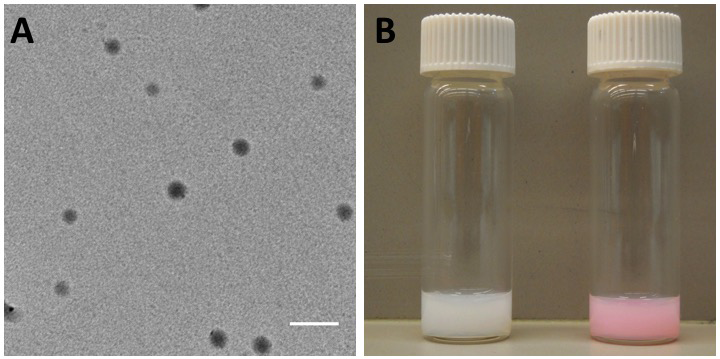
\includegraphics[width=\columnwidth]{photoactivation/particles}
    \caption{\label{fig:particles}Panel A shows a TEM image of PLGA nanoparticles after dehydration. The white scale bar is 200 \textmu m. Panel B shows the particles in suspension in water before (left) and after (right) UV light exposure, demonstrating the activation of the caged rhodamine.}
    \end{figure}
    
\subsubsection{Particle Characterization}
The diameter and $\zeta$-potential of the nanoparticles were determined by dynamic light scattering and laser Doppler electrophoresis, respectively, using a Zetasizer Nano ZS90 (Malvern Instruments, Southborough, MA). Transmission Electron Microscopy (TEM) images of dried particles were taken on standard 400 mesh copper TEM grids (TedPella, Redding, CA) with a Hitachi H7600 Electron Microscope. Particles were 160 $\pm$ 10 nm in diameter with a PDI of 0.11 $\pm$ 0.02 and a $\zeta$-potential of -3 $\pm$ 1 mV, where error bars report variation between batches.

\subsection{Sample Preparation}
\subsubsection{Fibrin gel}
Human fibrin gel was made from defrosted aliquots of thrombin and fibrinogen. Appropriate particle concentrations (between 0.005-0.00004\% by mass) for tracking PS-PEG or PLGA-PEG particles were made in 2 U/ml thrombin in PBS, with a total volume of 180 \textmu l. 20 \textmu l of 40 mg/ml fibrinogen was pipetted to the solution, yielding a 4 mg/ml concentration of fibrinogen\cite{Spero2011}. Vortex was immediately applied at high speed for ~2 s to homogenize the solution. 30 \textmu l of the solution was immediately pipetted into a 30 \textmu l well on a glass slide, covered with a glass coverslip, and sealed with a cyanoacrylate glue. The slide was then incubated at 37 �C for 20 min to ensure gelation. In all cases, slides were wrapped in aluminum foil to prevent premature exposure to UV light. 
\subsubsection{CF Sputum}
CFS was collected from adult patients at the Johns Hopkins Cystic Fibrosis Center in accordance with Institutional Review Board-approved protocols. Samples were stored at 4$^\circ$C immediately after collection, and were analyzed the next day. CFS slides were made according to a similar procedure as the above for fibrin gels: 30 \textmu l aliquots of CFS were withdrawn using a Wiretrol (Drummond Scientific Company, Broomall, PA) and injected into 30 \textmu l wells on glass slides. 1 \textmu l of appropriate particle suspensions for tracking or for photoactivation was added to the aliquot and mixed thoroughly. The slide was then sealed and allowed to incubate at room temperature for 1-2 hours (to prevent convection effects).  

\subsection{Measurements}           
\subsubsection{Multiple Particle Tracking (MPT)}
Particle motion in the CF sputum and fibrin samples was observed at room temperature using an inverted epifluorescence microscope (Axio Observer; Carl Zeiss, Thornwood, NY) with a 100X/1.46 NA oil-immersion objective. Movies were collected with 19-ms exposure at 20 fps for 500 frames using an EMCCD camera (Evolve 512; Photometrics, Tucson, AZ). Particle motion was tracked using the particle-tracking software described in Chapter \ref{chap:trackpy}.

\subsubsection{Confocal imaging and photoactivation}
Confocal imaging was performed on a Zeiss LSM510 laser scanning confocal microscope (Carl Zeiss, Thornwood, NY) in multi-tracking mode using either the 63x (Plan Apochromat 1.4 NA), 40x (PlanNeofluar 1.3 NA), or 20x (Plan Apochromat .75 NA) oil-immersion objective. Particles in the selected regions were activated by 10 to 25 iterations of the 405-nm laser at 100\% power, while particles were excited to fluorescence by the 543-nm laser at 10--30\%  power.   All videos were $512\times512$ pixels, and the activated region was $40\times512$ pixels. (For experiments performed using 20X, 40X and 63X objectives, this corresponds to $35\times449$, $18\times225$, or $11\times143$ \textmu m$^2$, respectively.)
Slide preparation for confocal experiments was identical to the above procedure for multiple particle tracking in CFS, with the exception of particle concentrations: PLGA-PEG particles were added to either water, CFS, or fibrin with final concentrations of 0.075\% to 0.03\% by mass. 


\section{Results}

\subsection{Water}

Here we obtain the particles' diffusivity $D$ in water from the evolution of the observed fluorescence intensity $I(x, y, t)$ from photoactivated particles. To begin, we will take the system to be homogenous, an assumption which of course holds for water, but which we must revisit when addressing more complex systems in later sections. Figure \ref{fig:water}(a) displays a series of fluorescence images at different times following UV exposure to a strip-shaped region of the sample indicated by the red lines in the top image. We take the $y$-direction to be parallel to the strip and the $x$-direction to be perpendicular to it. The experiment is symmetric along $y$, and so the full image $I(x, y, t)$ can be summarized by an intensity profile $I(x, t) = \sum_y I(x, y, t)$. Under carefully tuned experimental conditions, intensity is directly proportional to the concentration of activated particles $c(x, t)$. Of course, this approximation is not universally applicable: particles overlap and scatter incident light and the emitted light from the particles around them, so at high concentrations the observed intensity must ultimately saturate. Also, the sensor imposes a sharp limit of the range of observable intensities. A carefully designed experiment, then, must match the particle concentration $c$ and fluorescence (controlled in part by the intensity of incident light) to the sensitivity of camera. In our experiments, departures from the linear approximation $I \propto c$ were measurable but small, less than 5\%.

In a viscous liquid such as water, the concentration profile evolves according to the diffusion equation:

\begin{equation}
 \frac{\partial c}{\partial t} = D\frac{\partial^2 c}{\partial x^2}
\end{equation}

\noindent An idealized, infinitely thin activation region at $x'$ and time $t'$, described by $c(x) = \delta(x-x')$, would evolve as a Gaussian that spreads during some time interval $t-t'$ as

\begin{equation}
 c(x, t) = \frac{1}{\sqrt{4\pi D (t-t')}}\exp\left[-(x-x')^2/4D(t - t')\right]
\end{equation}

\noindent This Gaussian is the Green function $G(x - x'; t - t')$ for the diffusion equation. Therefore, for any distribution of activated particles $c(x', t')$ at time $t'$, the distribution at some later time $t$ will be

\begin{equation}
 \label{eqn:convolution}
 c(x, t) = \int_{-\infty}^\infty G(x - x'; t - t')\, c(x', t')\,dx'
\end{equation}

\noindent and therefore, if $I \propto c$,

\begin{equation}
 \label{eqn:convolution}
 I(x, t) = \int_{-\infty}^\infty G(x - x'; t - t')\, I(x', t')\,dx'.
\end{equation}

\noindent That is, the intensity profile at $t'$ can be mapped onto the intensity profile at $t$ through convolution with a Gaussian with width $\sigma=\sqrt{2D(t-t')}$. Breakdown of this mapping would indicate non-diffusive motion, which is not expected for water but could occur in other materials.

   \begin{figure}
    \centering
    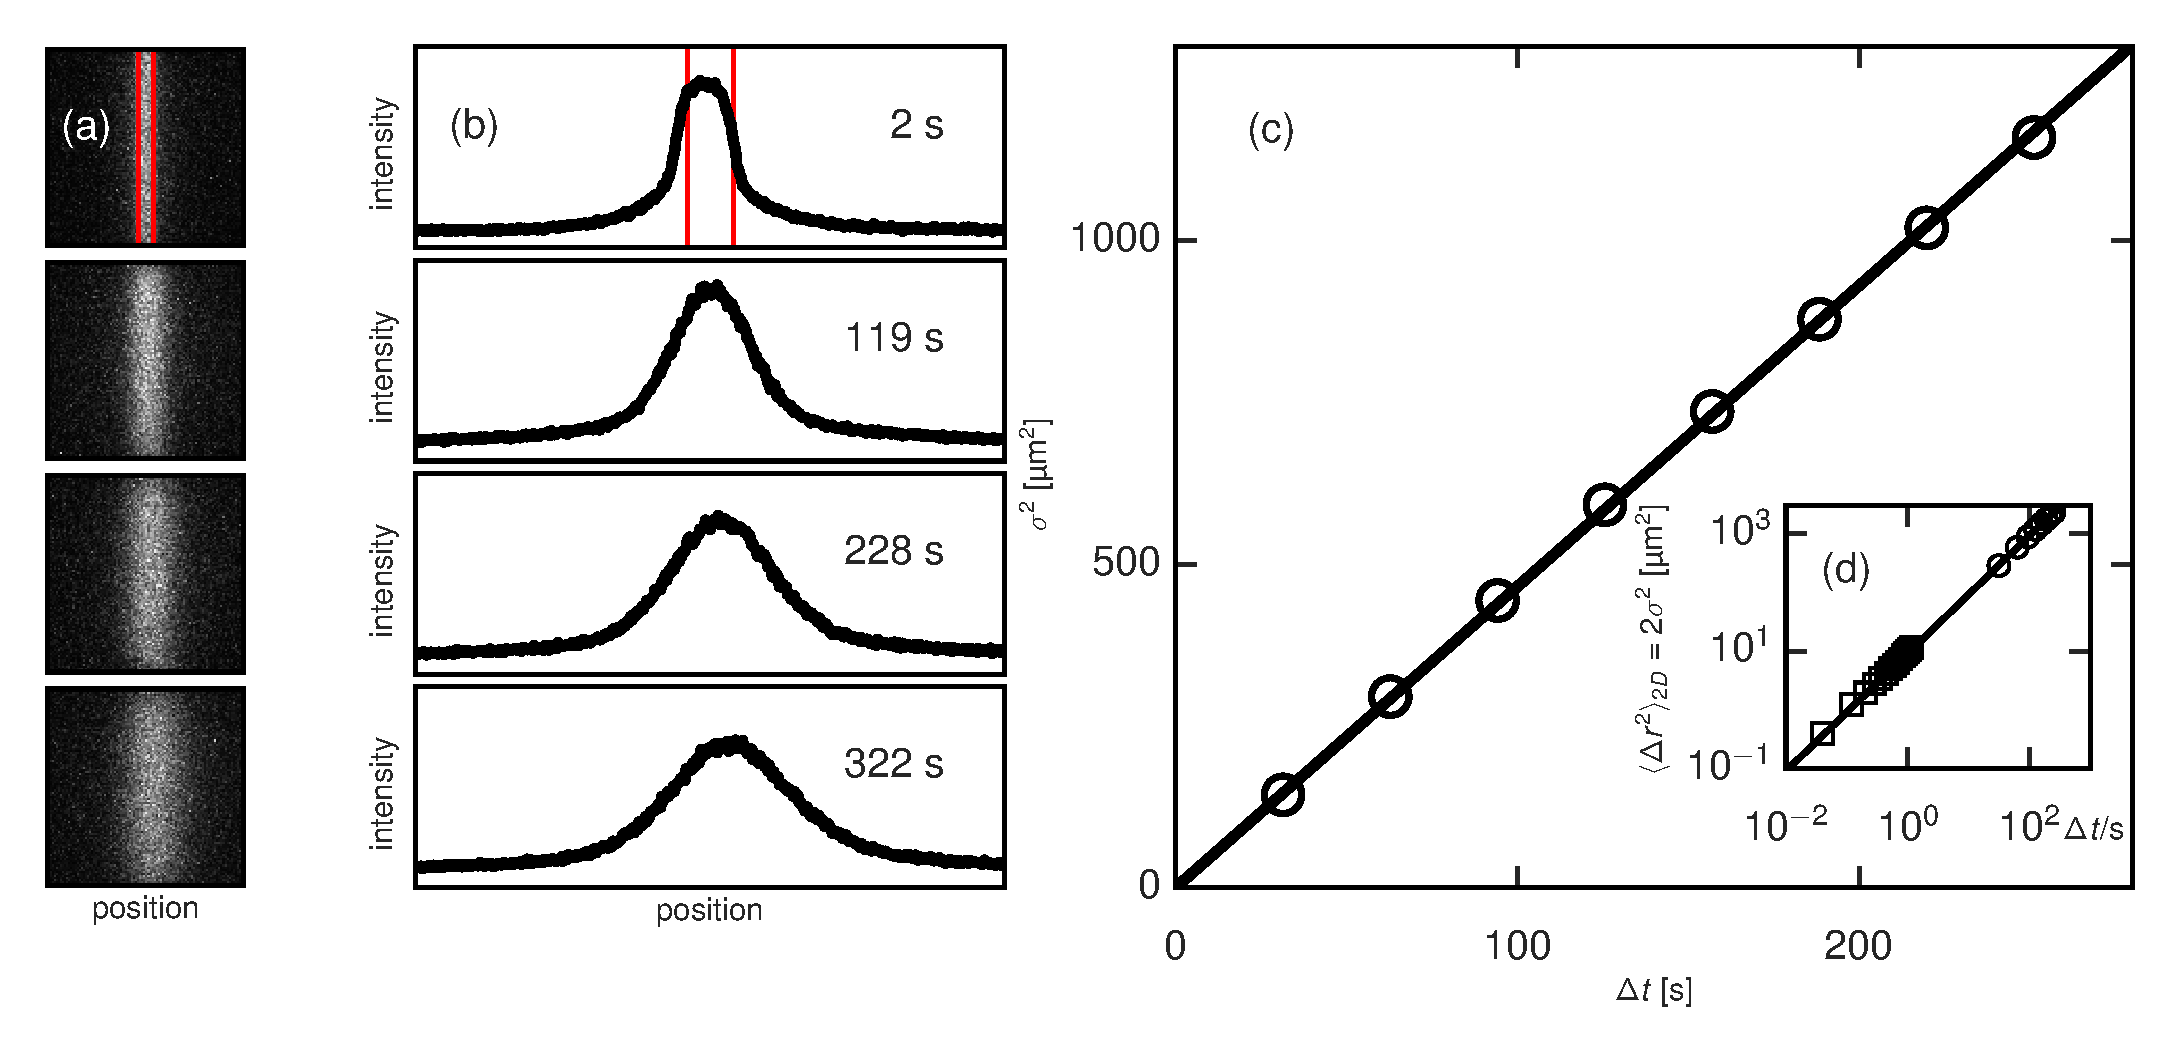
\includegraphics[width=\columnwidth]{photoactivation/water}
    \caption{\label{fig:water}Photactivatable nanoparticles diffuse in water. (a) The region outlined in red, which is 34 microns wide, is momentarily exposed to UV laser light, and any particles within that region become fluorescent. (b) Their subsequent diffusion is characterized by an intensity profile representing the summed intensity of each individual column in the image. Profiles at different times can be mapped onto each other through convolution with a Gaussian, as described in the text. (c) The Gaussian that maps a given profile at any $t'$ onto the profile at $t' + t$ has width $\sigma(t)$. This is related to the nanoparticles' diffusivity $D$ through $\sigma^2 = 2Dt$. We extract the value $D$=2.4 $\pm$ 0.1 \textmu m$^2$/s, which is within 5\% of the theoretical diffusivity of 170-nm particles in water at room temperature. (d) The particles were also studied using traditional multiple-particle-tracking (MPT), where all particles were activated and individually tracked in two dimensions. The mean-squared displacement of their trajectories $\langle \Delta r^2 \rangle_{2D}$ (squares) is shown alongside the Gaussian widths from (c), plotted once again as circles. The diffusivity obtained from MPT was $D$=2.421 \textmu m$^2$/s, in excellent agreement with the value obtained from photoactivation.}
    \end{figure}

During an experiment, hundreds of intensity profiles were captured at a regular interval. Every profile was mapped onto each future profile through convolution with a Gaussian, as in Eq. (\ref{eqn:convolution}). The width $\sigma$ of the Gaussian generating the most accurate mapping was determined using a nonlinear least-squares fit. Each mapping constituted a separate---though not strictly statistically independent---measurement of diffusivity $D$. Mappings corresponding to the same time interval $\Delta t = t - t'$ were averaged to produce the data points $\sigma^2(\Delta t)$ shown in Figure \ref{fig:water}(c). Finally, an estimate of $D$ was obtained through a linear regression to $\sigma^2(\Delta t)$. Its value, 2.4 $\pm$ 0.1 \textmu m$^2$/s, is within 5\% of the expected value for the diffusivity of 170-\textmu m particles in water, thus demonstrating the utility of the photoactivation approach as a microrheology technique. Figure \ref{fig:water}(d) shows the values of $\sigma^2$ from the photoactivation measurement along with those from MPT measurements. The two sets of results are consistent, and the figure indicates the complementary range of length and time scales each covers.

\subsection{Fibrin}

In experiments performed on samples of fibrin gel, some of the photoactivated nanoparticles spread with time outward from the activation region, but others remained immobilized, as evidenced by the still-bright activation region in Figure \ref{fig:fibrin-final-frame}, which depicts the intensity 785 seconds after photoactivation. The mobile and immobile populations can separated by comparing the full intensity profile $I(x, t=785\text{ s})$ to a Gaussian fit, where the fit is restricted to values of $x$ outside the initial activation region and extrapolated to within the activation region (Figure \ref{fig:fibrin-gaussian-portion}). Comparing the integrated area of the Gaussian to the excess intensity in the activation region, we estimate that the mobile particles make up 40\% of the total population. This fraction is compatible with our finding from MPT experiments in fibrin, which also show an approximately even split between mobile particles moving diffusively, $\langle \Delta r^2(t)\rangle \propto t$, and immobile particles characterized by a finite asymptotic MSD, $\langle \Delta r^2(t\rightarrow\infty)\rangle = \langle \Delta r^2 \rangle_0$. The MSDs of individual particles in fibrin derived from particle tracking are plotted in Figure \ref{fig:fibrin-msd}, illustrating this division of mobility into two populations. A histogram of $\langle \Delta r^2(t=1\text{ s})$, emphasizing the bimodal distribution of mobilities is shown in Figure \ref{fig:fibrin-msd-hist}.

We speculate that this bimodal distribution is a consequence of mesoscale heterogeneity in the fibrin gel that forms as a result of microphase separation during the gelation process. As the fibrogen polymerizes, the polymer solution undergoes spinodal decomposition. The phase separation is arrested, however, by the cross linking that locks in a bicontinuous structure of high and lower concentration gel. The porosity of the high-concentration regions is smaller than the particles, such that the particles are trapped in the gel. The fluorescence images directly capture this microstructure of the fibrin gel---the underlying spatial distribution of a polymer-rich phase, containing entrained particles, and a polymer-poor phase, which is essentially a viscous liquid in which the particles freely diffuse. The apparent length scale of this micro-scale phase separation, visible in Figure \ref{fig:fibrin-final-frame}, is about 10 \textmu m, which is less than the typical linear spacing between particles in the MPT experiments. This result thereby illustrates another way in which photoactivation complements MPT: the higher particle densities in photoactivation experiments resolve underlying structural heterogeneity that gives rise to the dynamic heterogeneity in the MPT experiments. (MPT experiments cannot be performed at such high particle densities due to both experimental and fundamental limitations discussed in Chapter \ref{chap:methods}.)

   \begin{figure}
    \centering
    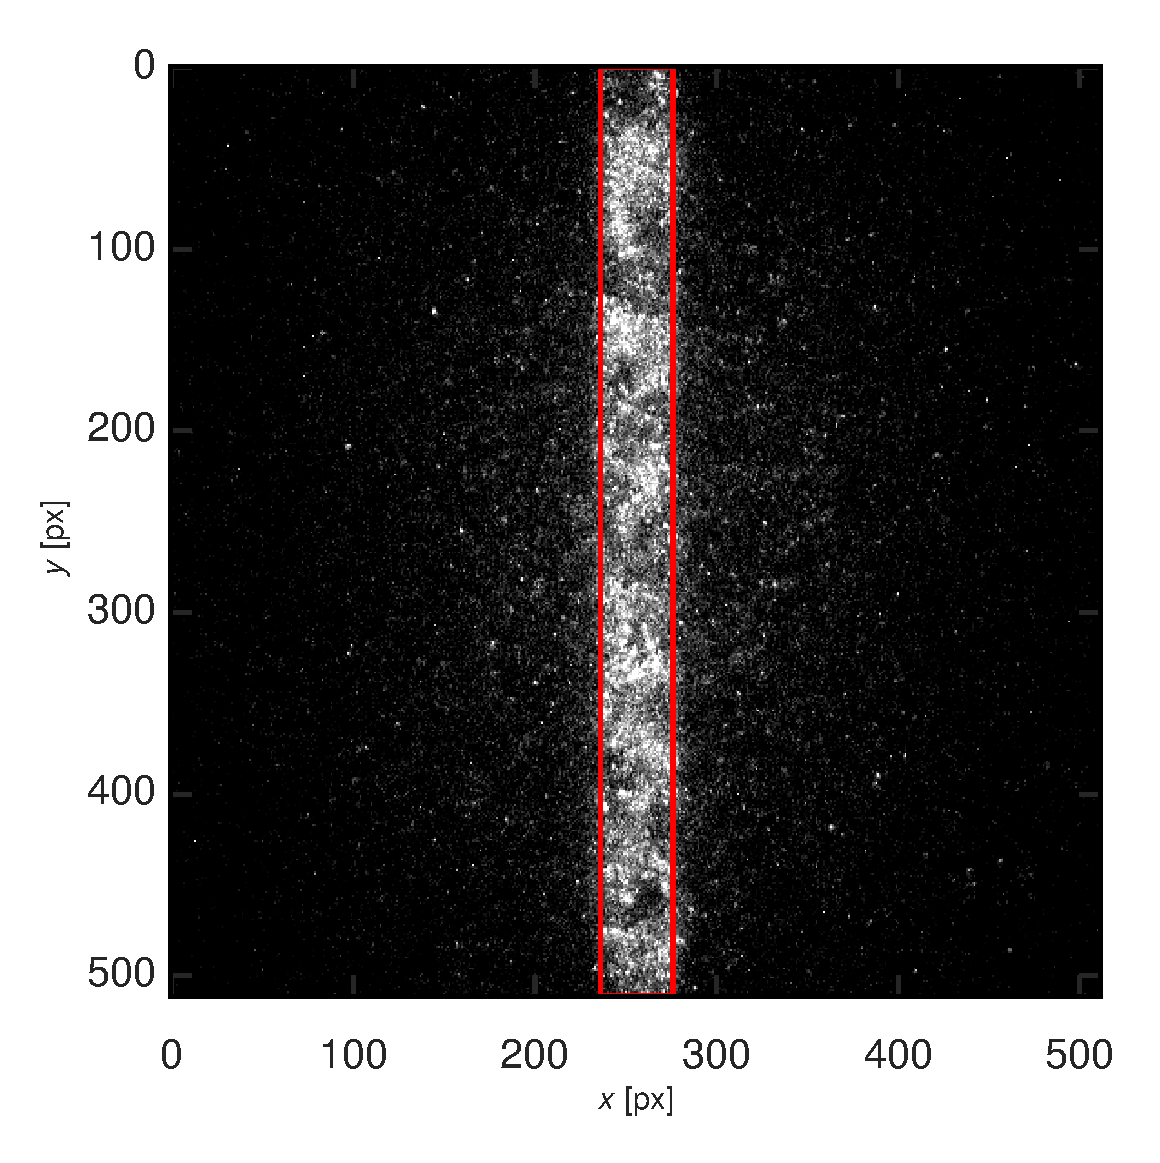
\includegraphics[width=\columnwidth]{photoactivation/fibrin-final-frame}
    \caption{\label{fig:fibrin-final-frame}Fluorescence intensity from photoactivated nanoparticles in fibrin 785 seconds after those in the activation region (outlined in red) were activated with UV light. While some have spread outward as in Figure \ref{fig:water}, the lingering intensity in the activation region shows that others remain immobilized in the immediate neighborhood of their initial position.}
    \end{figure}
    
   \begin{figure}
    \centering
    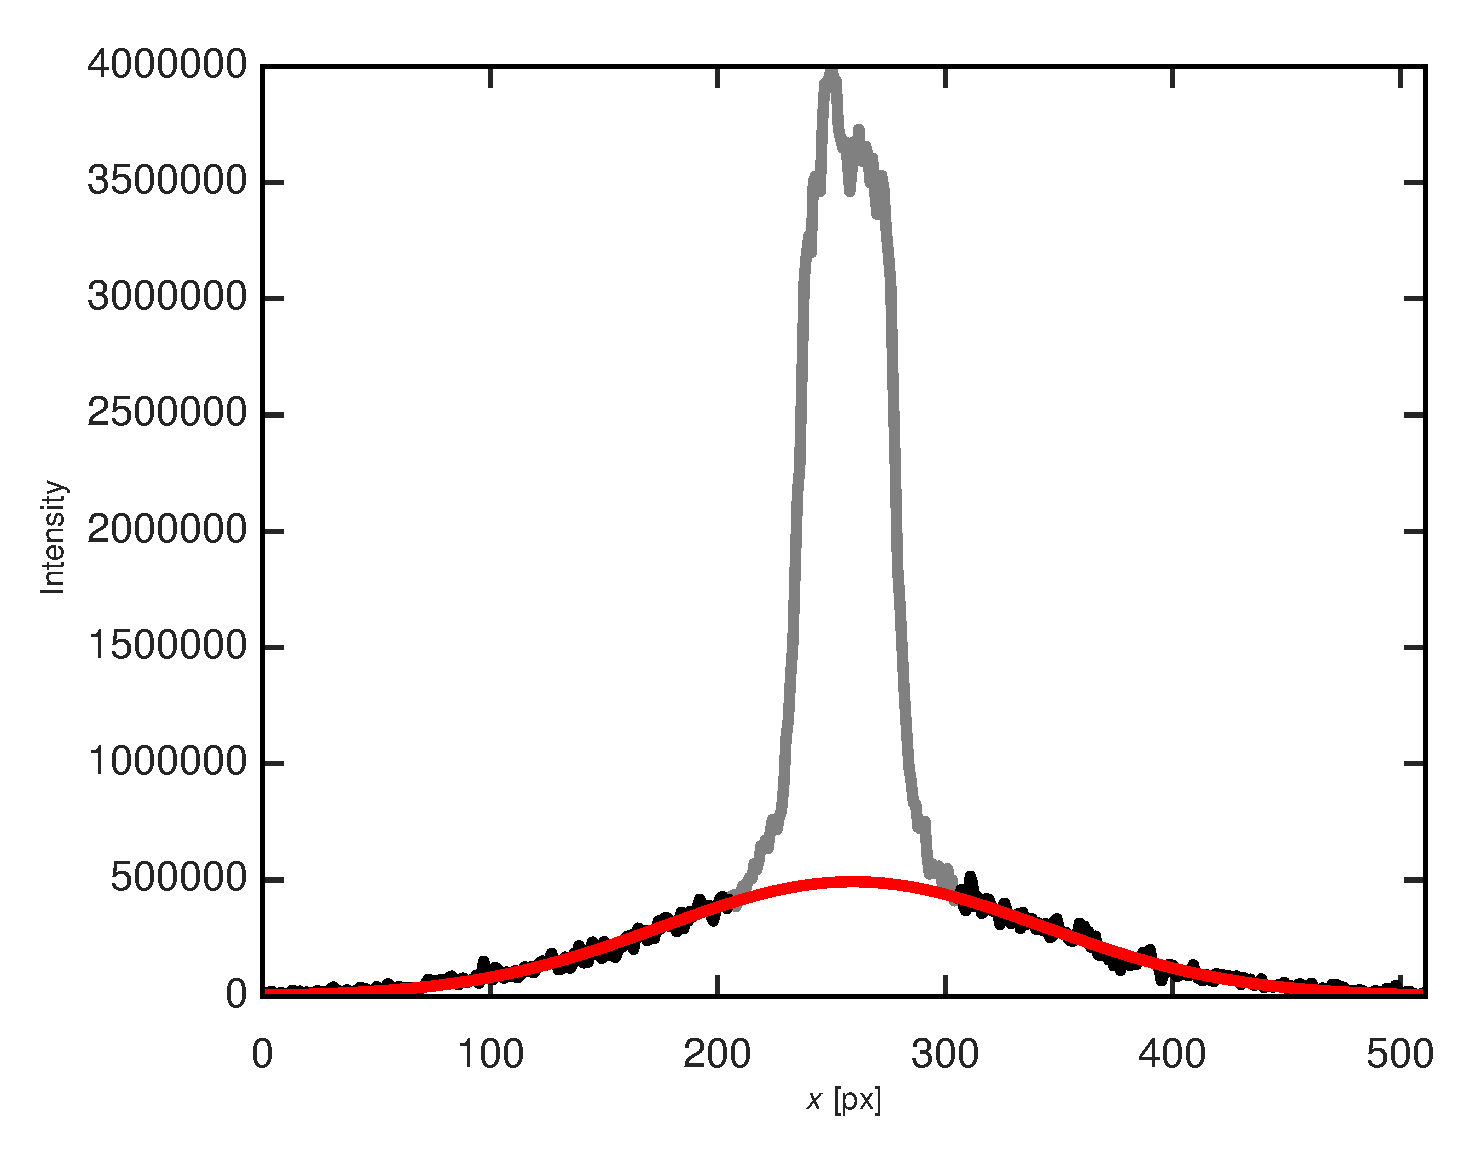
\includegraphics[width=\columnwidth]{photoactivation/fibrin-gaussian-portion}
    \caption{\label{fig:fibrin-gaussian-portion}The gray-and-black curve shows the intensity profile $I(x, t)$ at t=785 seconds. In red is a Gaussian, fit only to the black portion of $I$ outside the initial activation region. We posit that the intensity under the Gaussian is due to mobile particles that happen to be diffusing in that region while the intensity over the Gaussian is due to immobilized particles that are not diffusing.}
    \end{figure}
    
       \begin{figure}
    \centering
    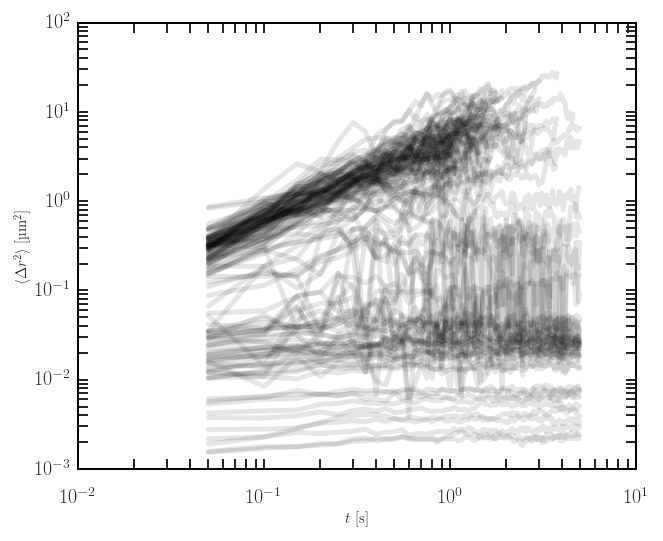
\includegraphics[width=\columnwidth]{photoactivation/fibrin-msd}    \caption{\label{fig:fibrin-msd}The MSD of individual PLGA-PEG particles in fibrin shows some particles moving diffusively and others jostling in place with an asymptotic MSD.}
    \end{figure}
    
           \begin{figure}
    \centering
    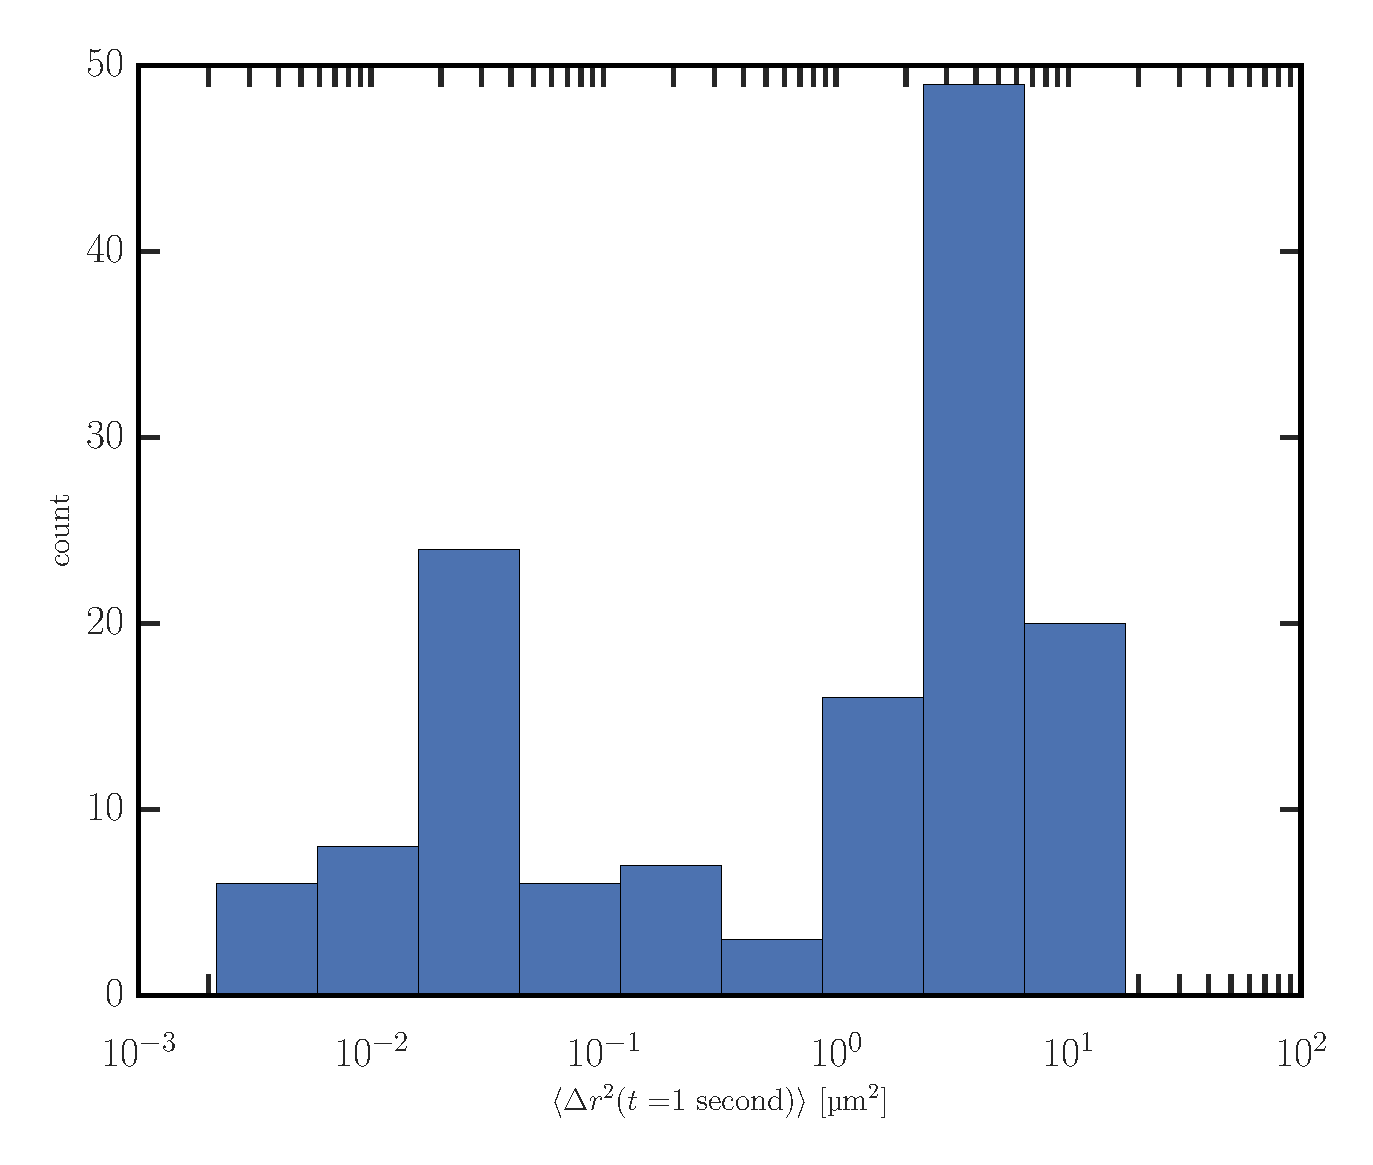
\includegraphics[width=\columnwidth]{photoactivation/fibrin-msd-hist}    \caption{\label{fig:fibrin-msd-hist}A histogram of the particles' MSD at lag time $t=$ 1 second shows an approximately equal division between mobile and immobile populations.}
    \end{figure}


\subsection{Cystic Fibrosis Sputum}

In particle-tracking studies, nanoparticles have been seen to diffuse through cystic fibrosis sputum (CFS)\cite{Schuster2013,Wang2008} over several micrometers, but in a CF patient the mucus barrier can be 20--50 \textmu m thick, or more, so it is important to show that nanoparticles can actually traverse tens of microns, the distance necessary to deliver therapeutic nanoparticles to lung cells. Heterogeneity in CFS has been seen in these particle-tracking studies, and it is unknown what impact this heterogeneity has on the long-distance mobility of nanoparticles in the sputum.

In addition to heterogeneity within a sputum sample, there is also patient-to-patient variation, which has been found to be the larger of these two effects\cite{SchusterThesis}. Characterization of nanoparticle mobility must contend with these variations. In our study, samples from one patient were found to be spatially homogeneous and approximately Newtonian. Thus, they were amenable to the same analysis performed on water above, as shown in Figure \ref{fig:simple-cfs}. From this analysis, we extract the diffusion coefficient $D=0.3994$ \textmu m$^2$/s, about an order of magnitude smaller than that in water.

   \begin{figure}
    \centering
    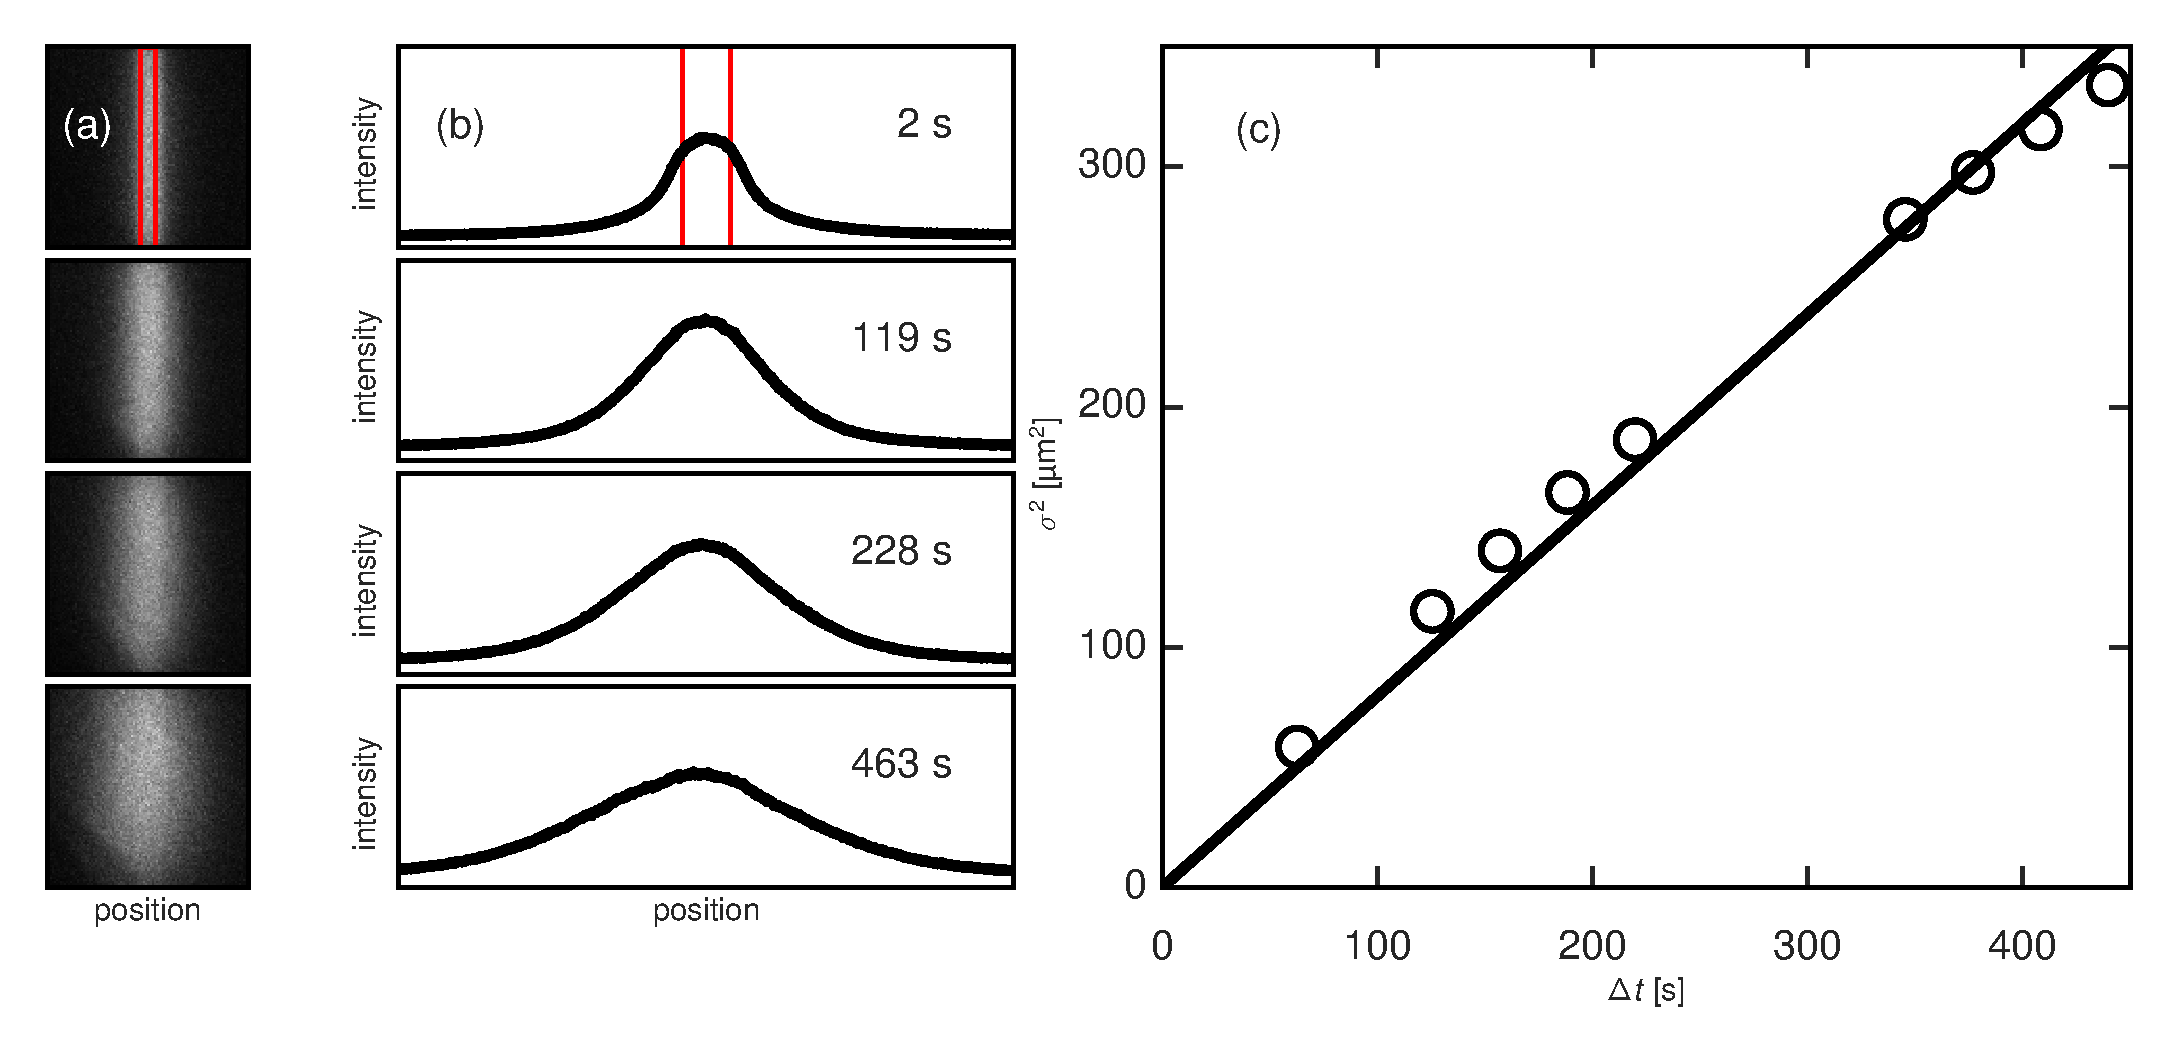
\includegraphics[width=\columnwidth]{photoactivation/simple-cfs}
    \caption{\label{fig:simple-cfs}Photactivatable nanoparticles diffuse in sputum collected from a human cystic fibrosis patient. As in Figure \ref{fig:water}: (a) The region outlined in red, which is 34 microns wide, is momentarily exposed to UV laser light, and any particles within that region become fluorescent. (b) Their subsequent diffusion is characterized by an intensity profile representing the summed intensity of each individual column in the image. Profiles at different times can be mapped onto each other through convolution with a Gaussian, as described in the text. (c) The Gaussian that maps a given profile at any $t'$ onto the profile at $t' + t$ has width $\sigma(t)$. This is related to the nanoparticles' diffusivity $D$ through $\sigma^2 = 2Dt$. We extract the value $D=0.3944$ \textmu m$^2$/s. (Missing data points are due to technical problems with video capture that, unfortunately, intermittently affected this particularly interesting trial.)}
    \end{figure}

Nanoparticle motion in samples from other patients was more complex and less amenable to straightforward application of such analysis. We observed mesoscale spatial heterogeneity, breaking the $y$-symmetry of the system, wherein the spreading particles made greater progress in certain subregions of the field of view. Illustrative examples are shown in Figure \ref{fig:cfs-gallery}. On a basic level, we see that nanoparticles can traverse tens of micrometers, so from a practical point of view this shows that it is possible for a PEG-coated nanoparticles to traverse CF sputum over a distance necessary to deliver therapeutic nanoparticles. To our knowledge, this is a new result. Of course, from the uneven permeability observed in Figure \ref{fig:cfs-gallery}, that delivery seems likely to be uneven across regions of the lung. Further, as with fibrin, photoactivation reveals the underlying microstructure of permeability that is difficult to discern from MPT analysis.

   \begin{figure}
    \centering
    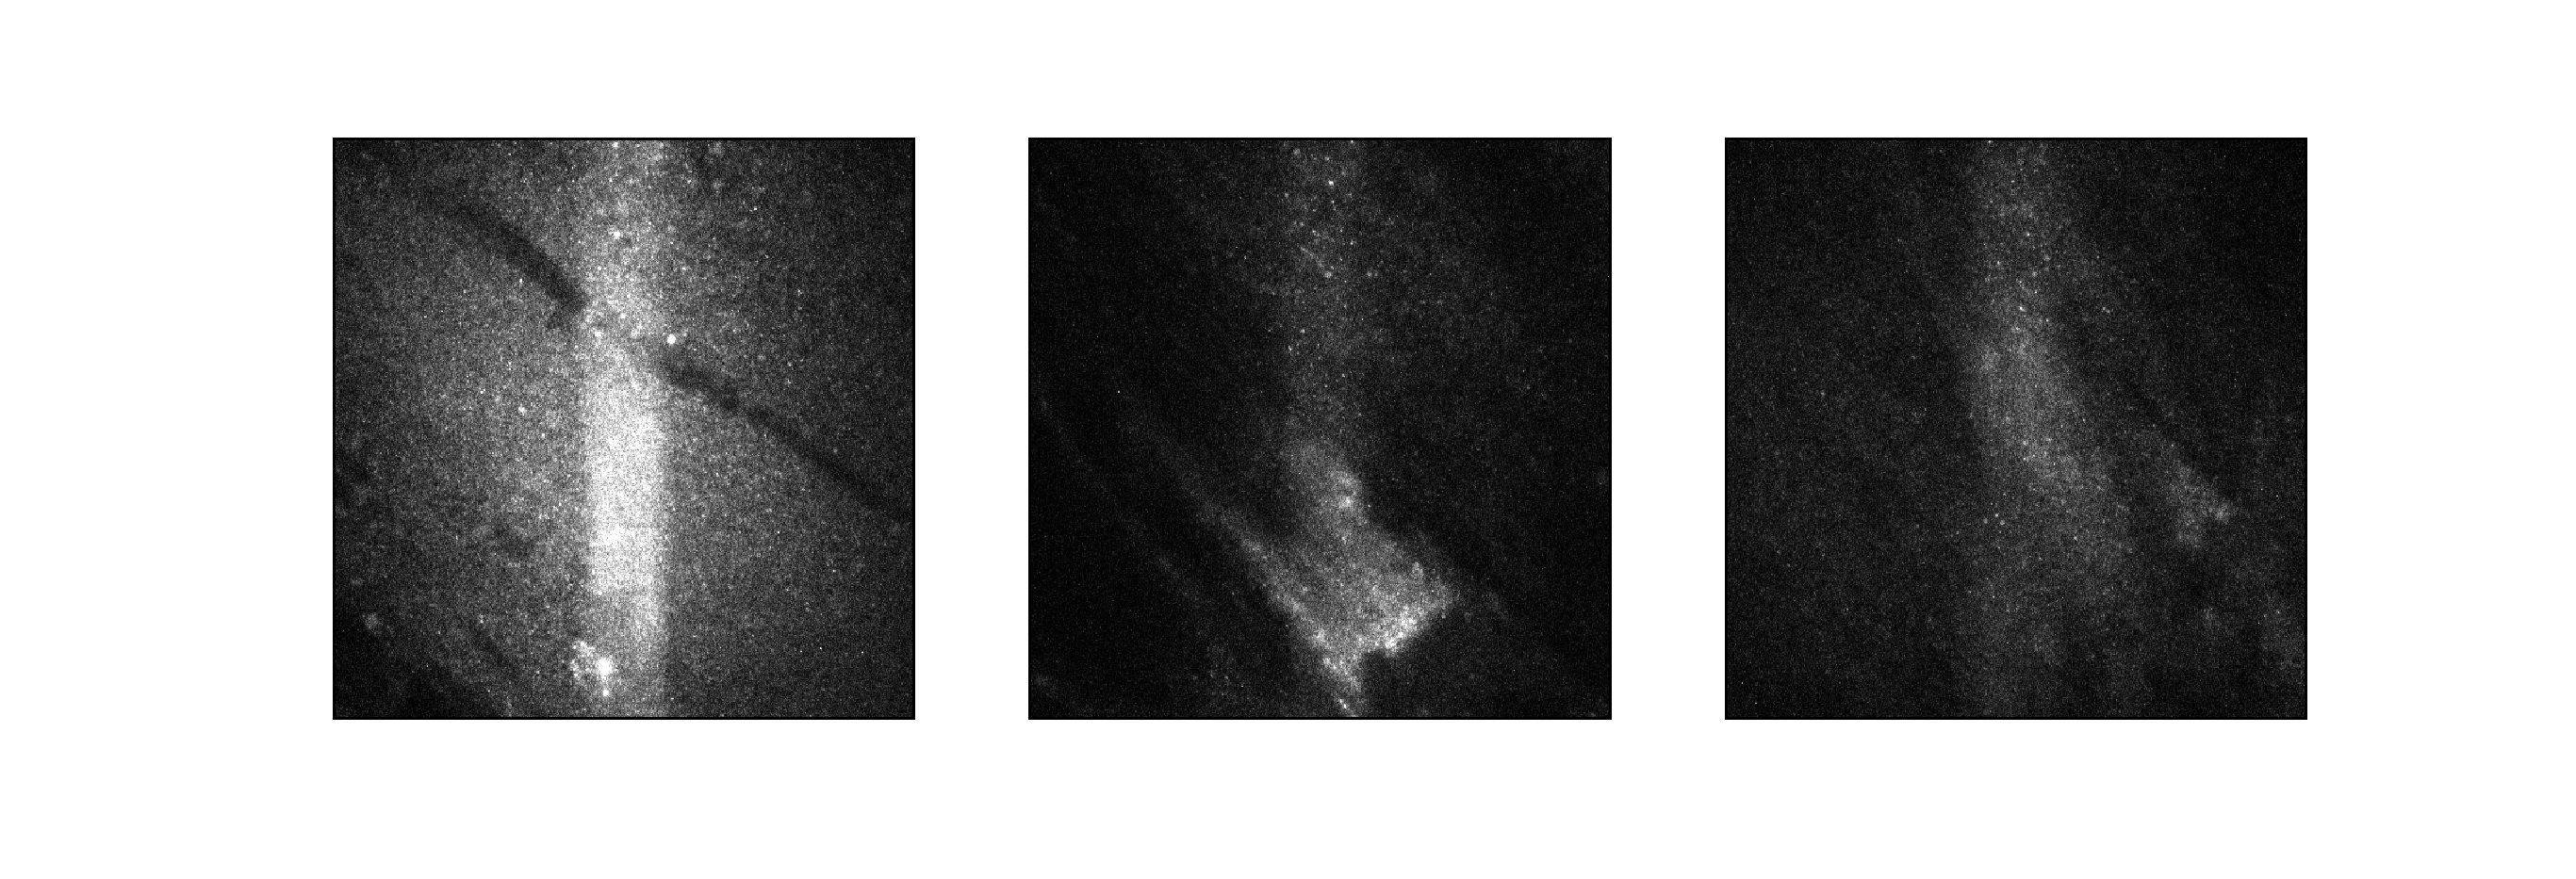
\includegraphics[width=\columnwidth]{photoactivation/cfs-gallery}
    \caption{\label{fig:cfs-gallery}In samples from some patients, dramatic heterogeneity was observed. These images depect the fluorescence intensity of photoactivated nanoparticles in three different samples from the same patient. At left, long substructures in the fluid are not permeated by the nanoparticles. At center, the particles spread more easily in the region at the lower-right part of the frame. At right, both of these kinds of effects are evident. The left and right images are taken 600 seconds (10 minutes) after activation; the center, 1570 s.}
    \end{figure}

\section{Discussion \& Conclusion}

We have developed a strategy of combining MPT with photoactivation for measuring nanoparticle diffusion in biological gels over multiple scales, ranging in time from tens of milliseconds to tens of minutes, and ranging in length from less than one micrometer to hundreds of micrometers.

The two techniques offer complimentary strengths. Particle tracking permits analysis of individual particles, and at high spatial and temporal resolutions, but the time and length of observation are limited. The photoactivation technique can monitor diffusion over longer times and distances, which are relevant in many drug-delivery applications, although spatial and temporal resolutions are not as good. Importantly, particle-tracking suffers from a sampling bias toward immobile particles, which stay in view longer and thus make up a disproportionate fraction of trackable particles\cite{Crocker2007}. The photoactivation technique, taking a wider view, captures the leading edge of diffusion and does not suffer from that particular bias.

In water, results from particle tracking and the photoactivation technique agree quantitatively. In fibrin, the two techniques portray compatible pictures of heterogeneous nanoparticle mobility. Finally, we directly observed PEG-coated PLGA nanoparticles diffusing over physiological distances in CFS and quantitified their diffusivity for one particular case that was unusually amenable to straightforward analysis. These findings extend prior, related work from the Hanes lab\cite{Schuster2013}.

\begin{appendices}
\chapter{Appendix}

\section{Trackpy Documentation}
\section{PIMS Documentation}
\section{Needle Documention}

\end{appendices}

%% REFERENCES

% if you use BIBTEX
\bibliographystyle{IEEEtran}
\bibliography{library/library,manually-entered-refs}

\begin{vita}

\begin{wrapfigure}{l}{0pt}
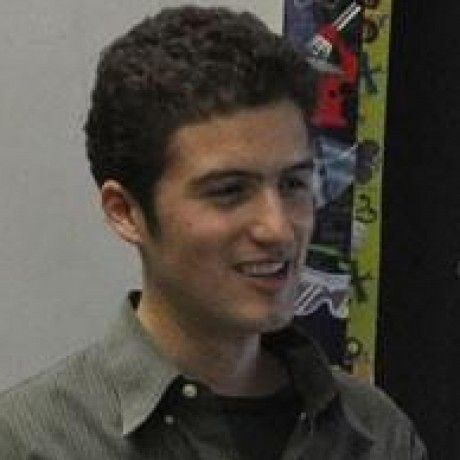
\includegraphics[width=2in,height=2.5in,clip,keepaspectratio]{dba-headshot}
\end{wrapfigure}

Dan is Dan.

\end{vita}
\end{document}
